\documentclass[twoside,11pt]{article}
\usepackage{jair, theapa, rawfonts}

\usepackage{color}
\usepackage{graphicx}
\usepackage{amssymb}
\usepackage{enumerate}
\usepackage{multirow}
\usepackage{siunitx}
\usepackage{url}

\usepackage{subfigure}
\usepackage{caption}
\usepackage{amsmath}
\let\chapter\section
\usepackage[ruled]{algorithm2e}

\usepackage{diagbox}

%  \usepackage{algorithm}
% \usepackage{algorithmic}
\usepackage{color,xcolor}

\usepackage{colortbl}
\usepackage{booktabs}

\jairheading{1}{1993}{1-15}{6/91}{9/91}
\ShortHeadings{On Forgetting in \CTL}
{Feng, Acar, Wang,  Liu, \& Schlobach}
\firstpageno{1}


\begin{document}

\newcommand{\tuple}[1]{{\langle{#1}\rangle}}
\newcommand{\Mod}{\textit{Mod}}
\newcommand\ie{{\it i.e. }}
\newcommand\eg{{\it e.g.}}
\newcommand\st{{\it s.t. }}
%\renewcommand{\st}{s.t.}
\newtheorem{definition}{Definition}
\newtheorem{examp}{Example}
\newenvironment{example}{\begin{examp}}{\end{examp}}
\newtheorem{lemma}{Lemma}
\newtheorem{proposition}{Proposition}
\newtheorem{theorem}{Theorem}
\newtheorem{corollary}[theorem]{Corollary}
\newenvironment{proof}{{\bf Proof:}}{\hfill\rule{2mm}{2mm}\\ }
\newcommand{\rto}{\rightarrow}
\newcommand{\lto}{\leftarrow}
\newcommand{\lrto}{\leftrightarrow}
\newcommand{\Rto}{\Rightarrow}
\newcommand{\Lto}{\Leftarrow}
\newcommand{\LRto}{\Leftrightarrow}
\newcommand{\Var}{\textit{Var}}
\newcommand{\Forget}{\textsc{F}}
\newcommand{\KForget}{\textit{KForget}}
\newcommand{\TForget}{\textit{TForget}}
%\newcommand{\forget}{\textit{forget}}
\newcommand{\Fst}{\textit{Fst}}
\newcommand{\dep}{\textit{dep}}
\newcommand{\term}{\textit{term}}
\newcommand{\literal}{\textit{literal}}
\newcommand{\Unfolding}{\textsc{uf}}

\newcommand{\Atom}{\mathcal{A}}
\newcommand{\SFive}{\textbf{S5}}
\newcommand{\MPK}{\textsc{k}}
\newcommand{\MPB}{\textsc{b}}
\newcommand{\MPT}{\textsc{t}}
\newcommand{\MPA}{\forall}
\newcommand{\MPE}{\exists}

\newcommand{\DNF}{\textit{DNF}}
\newcommand{\CNF}{\textit{CNF}}

%\newcommand{\degree}{\textit{degree}}
\newcommand{\sunfold}{\textit{sunfold}}

\newcommand{\Pos}{\textit{Pos}}
\newcommand{\Neg}{\textit{Neg}}
\newcommand\wrt{{\it w.r.t.}}
\newcommand{\Hm} {{\cal M}}
\newcommand{\Hw} {{\cal W}}
\newcommand{\Hr} {{\cal R}}
\newcommand{\Hb} {{\cal B}}
\newcommand{\Ha} {{\cal A}}
\newcommand{\Hi} {{\cal I}}
\newcommand{\Ind} {{\cal I}}
\newcommand{\GAL}{\textsc{gal}}

\newcommand{\Dsj}{\triangledown}
\newcommand{\Diff}{\textrm{Diff}}

\newcommand{\wnext}{\widetilde{\bigcirc}}
\newcommand{\nex}{\bigcirc}
\newcommand{\ness}{\square}
\newcommand{\qness}{\boxminus}
\newcommand{\wqnext}{\widetilde{\circleddash}}
\newcommand{\qnext}{\circleddash}
\newcommand{\may}{\lozenge}
\newcommand{\qmay}{\blacklozenge}
\newcommand{\unt} {{\cal U}}
\newcommand{\since} {{\cal S}}
\newcommand{\SNF} {\textit{SNF$_C$}}
\newcommand{\start}{\textbf{start}}
\newcommand{\Elm}{\textit{Elm}}
\newcommand{\simp}{\textbf{simp}}
\newcommand{\nnf}{\textbf{nnf}}

\newcommand{\CTL}{\textrm{CTL}}
%\newcommand{\Ind}{\textrm{Ind}}
\newcommand{\Tran}{\textrm{Tran}}
\newcommand{\Sub}{\textrm{Sub}}
\newcommand{\NI}{\textrm{NI}}
\newcommand{\Inst}{\textrm{Inst}}
\newcommand{\Com}{\textrm{Com}}
\newcommand{\Rp}{\textrm{Rp}}
\newcommand{\forget}{{\textsc{f}_\CTL}}
\newcommand{\ALL}{\textsc{a}}
\newcommand{\EXIST}{\textsc{e}}
\newcommand{\NEXT}{\textsc{x}}
\newcommand{\FUTURE}{\textsc{f}}
\newcommand{\UNTIL}{\textsc{u}}
\newcommand{\GLOBAL}{\textsc{g}}
\newcommand{\UNLESS}{\textsc{w}}
\newcommand{\Def}{\textrm{def}}
\newcommand{\IR}{\textrm{IR}}
\newcommand{\Tr}{\textrm{Tr}}
\newcommand{\dis}{\textrm{dis}}
\def\PP{\ensuremath{\textbf{PP}}}
\def\NgP{\ensuremath{\textbf{NP}}}
\def\W{\ensuremath{\textbf{W}}}
\newcommand{\Pre}{\textrm{Pre}}
\newcommand{\Post}{\textrm{Post}}


\newcommand{\CTLsnf}{{\textsc{SNF}_{\textsc{ctl}}^g}}
\newcommand{\ResC}{{\textsc{R}_{\textsc{ctl}}^{\succ, S}}}
\newcommand{\CTLforget}{{\textsc{F}_{\textsc{ctl}}}}
\newcommand{\WForget}{{\textsc{WF}_{\textsc{ctl}}}}
\newcommand{\degex}{{\textsc{def}_{\textsc{ex}}}}
\newcommand{\Refine}{\textsc{Refine}}
\newcommand{\cf}{\textrm{cf.}}
\newcommand{\NEXP}{\textmd{\rm NEXP}}
\newcommand{\EXP}{\textmd{\rm EXP}}
\newcommand{\coNEXP}{\textmd{\rm co-NEXP}}
\newcommand{\NP}{\textmd{\rm NP}}
\newcommand{\coNP}{\textmd{\rm co-NP}}
\newcommand{\Pol}{\textmd{\rm P}}
\newcommand{\BH}[1]{\textmd{\rm BH}_{#1}}
\newcommand{\coBH}[1]{\textmd{\rm co-BH}_{#1}}
\newcommand{\Empty}{\emptyset}%\varnothing}
\newcommand{\NLOG}{\textmd{\rm NLOG}}
\newcommand{\DeltaP}[1]{\Delta_{#1}^{p}}
\newcommand{\PIP}[1]{\Pi_{#1}^{p}}
\newcommand{\SigmaP}[1]{\Sigma_{#1}^{p}}


\newcommand{\authorComment}[3]
{{\color{#1}\textbf{[\!\![\!\![\marginpar{\centering{\color{#1}\textbf{#2}}}~ #3 ]\!\!]\!\!]}}}
\newcommand{\Renyan}[1]{\textcolor{red}{#1}}
\newcommand{\Yisong}[1]{\textcolor{blue}{#1}}
\newcommand{\Wanwei}[1]{\textcolor{magenta}{#1}}

	\title{Computing Sufficient and Necessary Conditions in CTL: \\A Forgetting Approach}

\author{\name Renyan Feng \email renyan\_feng@163.com \\
	\addr Guizhou University, P. R. China
	\AND
	\name Erman Acar$^*$ \email Erman.Acar@vu.nl \\
	%   \addr NASA Ames Research Center, Mail Stop: 244-7,\\
	%   Moffett Field, CA  94035 USA
	% \AND
%	\name Stefan Schlobach \email k.s.schlobach@vu.nl \\
	\addr Vrije Universiteit Amsterdam, The Netherlands\\
Civic AI Lab Amsterdam, The Netherlands
	\AND
	\name Yisong Wang$^*$ \email yswang@gzu.edu.cn \\
	\addr Guizhou University, P. R. China
	\AND
	\name Wanwei Liu \email wwliu@nudt.edu.cn \\
	\addr National University of Defense Technology, P. R. China
	\AND
	\name Stefan Schlobach \email k.s.schlobach@vu.nl \\
	\addr Vrije Universiteit Amsterdam, The Netherlands
}

% For research notes, remove the comment character in the line below.
% \researchnote

\maketitle


\begin{abstract}
Computation tree logic (\CTL) is one of the most common specification languages in the field of formal verification.
%to express a property that a system at hand is expected to satisfy.
In systems design and verification, it is  often important to update existing knowledge with new attributes and subtract the irrelevant information without altering the relevant system behaviour or violating the existing specifications over a given signature.  In such a scenario,  although they do not always exist for \CTL, the computation of two informative dual notions are very crucial: the strongest necessary condition (SNC) and the weakest sufficient
condition (WSC) of a given property in which the former corresponds to the most general consequence and the latter corresponds to the most specific abduction.
%Abstract a piece of information without altering the relevant system behavior or violating the existing specifications over a given signature, update existing knowledge with new attributes,
%and calculate a (the weakest) precondition that is sufficient for a transition system to enjoy the desired property.
In this article, we address these scenarios for \CTL\ in a principled way in terms of knowledge {\em forgetting}.\footnote{This paper is the revised and extended version of a paper which appeared in the Proceedings of KR 2020~\cite{renyansfirstpaper}.}
In particular, we propose a
model-theoretic notion of forgetting by a generalized bisimilar equivalence (over a signature) and explore
its general properties, i.e., modularity, commutativity, and homogeneity, as a knowledge distilling operator, and  show how to obtain SNC, WSC and the knowledge update via forgetting. We present a representation theorem for forgetting in bounded \CTL, based on Zhang-Zhou's postulates.
Furthermore, we complement our model-theoretic approach  with a more efficient syntactic one; a resolution-based method, to compute the forgetting in \CTL. We run our Prolog implementation on both \CTL-RP benchmark and a randomly generated \CTL\ dataset.
%More importantly, it refers to that the forgetting in bounded \CTL\ can be characterized by Zhang-Zhou's four postulates by a representation theorem and gives a model-based algorithm to compute such forgetting.
%It then shows how the weakest sufficient condition and the knowledge update can be established by forgetting.
% It also discusses the relationship between weak forgetting and the (strong) forgetting.
Our experimental results suggest that the number of atoms to be forgotten has a high impact on the performance of the algorithm.
% Moreover,  our algorithm  computes SNC 100\% of the cases for propositional logic, while it remains   ~80\% for  \CTL\ (provided that it might also not exist).

% \textcolor{red}{Computation tree logic (\CTL) is one of the most well-studied specification languages in the field of formal verification. In the field of system design and verification, often times it is important to subtract the irrelevant information without altering the relevant system behaviour or violating the existing specifications over a given signature.
% In such a scenario, two crucial notions are informative: the strongest necessary condition (SNC) and the weakest sufficient
% condition (WSC) of a given property.
% This paper addresses these scenarios for \CTL\ in a principled way in terms of knowledge {\em forgetting}.
% In particular, it proposes a notion of forgetting by a generalized bisimilar equivalence (over a signature) and explores
% it's general properties. %, i.e., modularity, commutativity, and homogeneity, as a knowledge distilling operator.
% And it also explores a resolution-based method to compute the forgetting in \CTL.
% More importantly, it refers to that the forgetting in bounded \CTL\ can be characterized by Zhang-Zhou's four postulates by a representation theorem and gives a model-based algorithm to compute such forgetting.
% It then shows how the WSC and the knowledge update can be established by forgetting.
% % It also discusses the relationship between weak forgetting and the (strong) forgetting.
% Moreover, experimental results show that the more atoms to be forgotten slower the calculation speed. And the SNC computed by our forgetting method always exists in propositional logic (PL) and in most cases of \CTL\ (it is about 80\% in the best situation).
% }
\end{abstract}

\section{Introduction}
\label{Introduction}

Computation tree logic (\CTL)~\cite{clarke1981design} is one of the central formalisms in formal verification. As a specification language, it is used to express a property
that the system at hand is expected to satisfy.
From both the verification and the system design points
of view,  there might be situations in which some information content of such property might become irrelevant for the system due to various reasons, e.g., it might be discarded or become obsolete by time, or just  become infeasible due to practical difficulties. As keeping such irrelevant information would be undesirable (such as waste of computational resources), the problem arises on how to remove it without altering the
relevant system behavior or violating the existing system
specifications over a given signature. Consider the following example.
\begin{figure*}[ht]
	\centering
	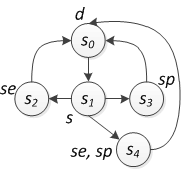
\includegraphics[width=4cm]{NnewCar.png}\\
	\caption{Car engine manufacturing scenario}\label{BVM}
\end{figure*}
\begin{example}[Car-Manufacturing Company]\label{car_manufacturing}
	Assume a car-manufacturing company which produces two types of cars: a (se)dan car and a (sp)orts car. In each manufacturing cycle, the company has to (s)elect one of the three options: (1) produce $se$  first, and then $sp$; (2) produce $sp$ first, and then $se$; (3) produce $se$ and $sp$ at the same time. At the first of each selection, a (d)ecision is taken, i.e., given all the reasonable plans. This schematic view of this scenario is illustrated in Figure~\ref{BVM}, as a  Kripke structure $\Hm=(S, R, L)$ with the initial state $s_0$ (called labeled state transition graph),  and the corresponding atomic variables $V=\{d,s,se,sp\}$.
	Now assume a situation in which due to some problems (e.g., economic crises or new environmental regulations on the engine technology) the company can no longer support the production of sports cars.
	This means that, all the manufacturing processes concerning $sp$ are not  necessary anymore. How should the company update the specification and the process (represented as a Kripke structure)?
	
	%and thus should be dropped from both the specifications and the Kripke structure.
	
	
\end{example}

 Similar scenarios may arise in many different application domains such as business-process modeling, software development, concurrent systems, and more~\cite{Baier:PMC:2008}. Yet given a signature, dropping some restrictions in a large  complex system  without affecting the working system components, or violating dependent specifications is a non-trivial task.
 Moreover, in such a scenario, two logical notions are highly informative: the \emph{strongest necessary condition} (SNC) and the \emph{weakest sufficient condition}  (WSC)  of a given specification~\cite{DBLP:Lin:AIJ:2001}.
 These correspond to the \emph{most general consequence} and the \emph{most specific abduction} of such specification, respectively.

In formal verification, Dijkstra proposed a method, called the weakest precondition calculus, to compute the \emph{weakest precondition}
(WP) in verifying a `Hoare triple' $\{\phi\} P \{\psi\}$, where $P$ is a program and both $\phi$ and $\psi$ are specifications~\cite{DBLP:journals/cacm/Dijkstra75}.
In a similar scenario,  given a model checking problem (i.e., deciding whether $\Hm \models \varphi$ for a given Kripke structure $\Hm$ and a specification $\varphi\in$ \CTL\ ), the problem of how to compute a \emph{precondition} $\psi$ over a given signature such that $\Hm \models \psi \rto \varphi$ whenever $\Hm \not \models \varphi$ is raised.
However, this cannot be computed by the method of Dijkstra since the given model $\Hm$ may be non-terminating.
Besides,  SP and the WP of a given specification are central to a wide variety of tasks and studies, e.g., in generating counterexamples~\cite{dailler2018instrumenting} and refining system~\cite{woodcock1990refinement} in verification.
So to speak, if we have such a WP, then updating the model $\Hm$ with the WP (or WSC) is natural.

% Moreover, for a given model checking problem, i.e., deciding whether $\Hm \models \varphi$ for a given Kripke structure $\Hm$ and a specification $\varphi$ (i.e., a \CTL\ formula), a problem is raised on how to compute a \emph{precondition} $\psi$ over a given signature such that $\Hm \models \psi \rto \varphi$ whenever $\Hm \not \models \varphi$.
% In a similar scenario, Dijkstra proposed a method, called the weakest precondition calculus, to compute the \emph{weakest precondition}
% (WP) in verifying a `Hoare triple' $\{\phi\} P \{\psi\}$~\cite{DBLP:journals/cacm/Dijkstra75}, where $P$ is a program and both $\phi$ and $\psi$ are specifications.
% However, this is not the case in model checking since the given model $\Hm$ may be non-terminating and cannot be computed by the method proposed by Dijkstra.
% Besides, as we have seen that
% the \emph{strongest post-condition} (SP) and the WP of a given specification are central to a wide variety of tasks and studies, e.g., in generating counterexamples~\cite{dailler2018instrumenting} and refining system~\cite{woodcock1990refinement} in verification.
% (It should be noted that the SP and WP correspond to the \emph{strongest necessary condition} (SNC) and the \emph{weakest sufficient condition}  (WSC)~\cite{DBLP:Lin:AIJ:2001}, of the specification, respectively.)

%   These correspond to the \emph{most general consequence} and the \emph{most specific abduction} of such specification, respectively.


Updating logical databases  traces back to Fagin et al.'s work in~\cite{DBLP:journals/acr/FaginKUV86}.
Various postulates are proposed for which arguably any plausible update function should satisfy. Among those postulates,  Katsuno and Mendelzon's postulates (U1)-(U8) ~\cite{katsuno91mendelzon}, are well-studied.
In ~\cite{baral2005knowledge}, the \emph{knowledge update} for modal logic S5 has been introduced, using the modal operator K (for agent \emph{knows}), and the proposed notion of update has been shown to satisfy Katsuno and Mendelzon's postulates.

%which extended the notion of belief update by solving the belief update caused by sensing actions, was proposed in
%in which the effect of a sensing action is expressed by ,
Using a forgetting-based method to update databases has been studied for propositional logic (PL) formulas in~\cite{DBLP:conf/aaai/FangWLFL18} and for atoms in modal logic S5 in~\cite{Yan:AIJ:2009}.
Nevertheless, to the best of our knowledge, the knowledge update of \CTL\ including temporal operators has not been explored so far.

To address these scenarios and target the relevant notions of SNC and WSC in a principled way,
%we employ a method based on formal verification.%\footnote{ This is  especially useful for abstracting away the domain-dependent problems, and focusing on conceptual ones.} In particular,
we introduce a \emph{forgetting}-based approach in \CTL\ and show that it can
be used to compute SNC and WSC on a restricted subset of the propositional variables, in the same spirit of~\cite{DBLP:Lin:AIJ:2001,DBLP:conf/ijcai/DohertyLS01}.
%And a resolution-based method is proposed to compute forgetting in \CTL.
In addition, we demonstrate that the knowledge update can  be computed by forgetting.

The \textbf{major contributions} of our paper are as follows:
\begin{itemize}
	\item We define the notion of forgetting in \CTL\ via the bisimulation on some set of atoms and explores its semantics properties, i.e., modularity, commutativity, and homogeneity.
	\item We explore a resolution-based method to compute forgetting in \CTL\ by using the resolution rules proposed in~\cite{zhang2014resolution}.
	To achieve this, we provide the notion of binary bisimulation (over a given signature and a set of indices) and an elimination process, including a generalized Ackermann’s lemma.
	Moreover, the theorem shows that some atoms introduced in the calculational process can not be eliminated from its result for some \CTL\ formulas, this follows that \CTL\ is a failure of uniform interpolation.
	%In order to prove the result of this method is
	%The main idea of this method is that it transforms a \CTL\ formula into its normal form, i.e., $\CTLsnf$,
	\item We outline a situation in which the forgetting is closed. To prove that it is closed, we define the characterizing formula (i.e., a \CTL\ formula) of the (finite) initial structure and show that each \CTL\ formula is equivalent to a disjunction of the characterizing formulas of its models.  This fact means that the result of forgetting some atoms from a \CTL\ formula always exists. Besides, we propose a model-based method to compute forgetting even if it is not very efficient, as one might expect. However, settling it is important from a theoretical point of view, to see how costly is the naive approach.
	\item We show that the WSC (SNC) and knowledge update can be obtained by using the forgetting technique. In particular, we prove that the WSC (SNC) of a specification (i.e., a \CTL\ formula) on a given signature under a (finite) initial structure can be obtained by expressing this structure with its characterizing formula. Moreover, we exhibit  the knowledge update defined by forgetting satisfies Katsuno and Mendelzon's postulates (U1)-(U8) proposed in~\cite{katsuno91mendelzon}.
	\item We have run our resolution-based algorithm (implemented in Prolog) on a set of \CTL\ formulas that both from the \CTL-RP benchmarks and generated randomly to complement these theoretical insights with empirical findings and obtain the SNC of the given formula.
\end{itemize}

The rest of the paper is organized as follows.
Section~\ref{related_work} reports on the related work.
Section~\ref{preliminaries} introduces the notation and technical preliminaries.
Section~\ref{forgetting_ctl} offers the notion of forgetting and its semantics properties. Moreover, it provides a resolution-based method to compute forgetting in Section~\ref{sec:resolution}.
%Section~\ref{forgetting_bounded} explores the model-based method for forgetting in bounded \CTL. In particular, it provides a model-theoretic characterization of \CTL\ for (initial) Kripke structures and shows that the forgetting in bounded \CTL\ is closed and satisfies the representation theorem. In addition, it gives a model-based algorithm for computing forgetting in bounded \CTL\ and discusses the relation between forgetting, SNC (WSC), and the knowledge update.
%Section 6 explores the relation between weak forgetting and (strong) forgetting.
Experimental results are shown in Section 7 to evaluate the Resolution-based method from an intuitive perspective.
The conclusion closes the paper. To avoid hindering the flow of content, proofs and the wearying constructions are moved into the Appendix.





\section{Related work}
\label{related_work}

This section surveys previous works which are closely related to this paper and are important in artificial intelligence.


\subsection{Forgetting}
To progress the knowledge of cognitive robotics, \emph{forgetting} was first formally presented in first order logic (FOL)~\cite{lin1994forget}. It can  be traced back to the work of Boole on propositional
variable elimination and the seminal work of quantifier elimination~\cite{ackermann1935untersuchungen}.
% Recently, forgetting has been extensively investigated from the perspective of Knowledge representation and reasoning,
% including description logics, that are subclasses of first order logic, modal logics and nonmonotonic logics.
% Alternative variants such as (\emph{strong/semantic}) forgetting, forgetting for simple, and \emph{weak} forgetting, respectively has been introduced in~\cite{Zhang:KR:2010}.
Noteworthy to mention is that forgetting is a dual notion of long-studied {\em uniform interpolation}~\cite{visser1996uniform,konev2009forgetting}.

In propositional logic (PL), {\em forgetting} a propositional variable $p$
from a  formula $\varphi$, written $\Forget(\varphi,\{p\})$, is the formula $\varphi[p/\bot] \vee \varphi[p/\top]$,
which is equivalent to $\exists p\varphi$~\cite{lin1994forget}.
%where %$\varphi[p/\top]$ (resp. $\varphi[p/\bot]$) is obtained from $\varphi$ by replacing
% every occurrence of $p$ in $\varphi$ with
% with
%$\top$ (true) and $\bot$ (false) respectively~\cite{lin1994forget}.
%
{\em Forgetting} a finite set $P$ of propositions from $\varphi$, written $\Forget(\varphi, P)$, is defined as: %  follows:
\begin{alignat}{2}
      &  \Forget(\varphi, \emptyset) = \varphi, \qquad % \nonumber \\
      &  \Forget(\varphi, P \cup \{q\})  = \Forget(\Forget(\varphi, \{q\}), P).
      \nonumber
\end{alignat}

In the context of FOL, forgetting has often been studied as an instance of the \emph{second-order quantifier elimination} (SOQE) problem. In particular, it has been shown that the result of (strong) forgetting of an $n$-ary predicate $P$ from a FOL formula $\varphi$ is the second-order formula $\exists R \varphi[P/R]$, in which $R$ is an $n$-ary predicate variable and $\varphi[X/Y]$ is the result of replacing every occurrence of $X$ in $\varphi$ by $Y$~\cite{lin1994forget}.
Hence, the task of forgetting in FOL is to find a first-order formula that is equivalent to $\exists R \varphi[P/R]$.
However, a second-order formula is possibly not expressible by a first-order one.
As an ontology engineering technique to produce {\em views} of ontologies,
forgetting has been widely explored in description logics (DLs), that are subclasses of first-order logic~\cite{Wang:AMAI:2010,Lutz:IJCAI:2011,Konev:JAIR:2012,Zhao:2017:IJCAI,DBLP:conf/aaai/ZhaoSWZF20}.


% \begin{itemize}
% 	\item $\Forget(\varphi, \emptyset) = \varphi$,
% 	\item $\Forget(\varphi, P \cup \{q\}) = \Forget(\Forget(\varphi, \{q\}), P)$.
% \end{itemize}

{\em Knowledge forgetting} was firstly proposed in the propositional modal logic S5 to reason about agents' epistemic states (knowledge or belief). In doing so, four general postulates were presented to precisely characterize the notion of knowledge forgetting~\cite{Yan:AIJ:2009}.
%
% In the context of modal logic (i.e., S5), authors of \cite{Yan:AIJ:2009}  define the \emph{knowledge forgetting} from the \emph{strong forgetting} point of view and explore  its relation to \emph{knowledge update}.  % by Yisong: Moreover, they show that \emph{uniform interpolation} ~\cite{visser1996uniform} is a dual concept of forgetting in S5 and PL.
% In doing so, they propose four general postulates (as we will revisit) and show that these four postulates precisely characterize the notion of knowledge forgetting in S5.  Moreover, they show that \emph{uniform interpolation} ~\cite{visser1996uniform} is a dual concept of forgetting in S5 and PL.  These notions were recently extended to multi-agent modal logics~\cite{fang2019forgetting}.
%
Furthermore, in the scenario of non-monotonic reasoning,  (Knowledge) {\em forgetting} in logic programs under answer set semantics has been extensively investigated from the perspective of various forgetting
postulates~\cite{DBLP:Zhang:AIJ2006,DBLP:journals/ai/EiterW08,Wong:PhD:Thesis,Yisong:JAIR,Yisong:IJCAI:2013,DBLP:journals/jair/Delgrande17}.%,gonccalves2020limits}
%see~\cite{eiter2019brief,gonccalves2020limits,gonccalves2021forgetting} for a comprehensive survey.
%for dealing with its different notions of “equivalence”, especially the strong equivalence, in which they proposed many kinds of operators to preserve equivalence in forgetting (while most of them are lose in preserving the strong equivalence).


% Noteworthy is that existing forgetting definitions in PL and answer set programming are not directly applicable in modal logics.
% Moreover, existing forgetting techniques are not directly applicable in \CTL\ either since it does not enjoy uniform  interpolation (implied by~\cite{Maksimova:JANCL:1991}). % by Yisong: either because there are some temporal operators in \CTL\ but not in S5.
% In our work we explore forgetting in \CTL\ from a strong point of view.
% In addition, similar to~\cite{Yan:AIJ:2009}, we research forgetting in bounded \CTL\ from the semantic forgetting point of view and show that the result of forgetting some propositions from a \CTL\ formula is always expressible in bounded \CTL.
% Furthermore, we show that our notion of forgetting in bounded \CTL\ satisfies those four postulates of forgetting presented in~\cite{Yan:AIJ:2009}.
% And last, we demonstrate how forgetting can be used to compute the SNC and WSC on a set of propositions and as the knowledge update.

\subsection{The Weakest Sufficient Condition (WSC)}
As aforementioned, the WSC and its dual notion of the strongest necessary condition (SNC) are highly crucial notions for formal verification in software engineering. Roughly speaking, the WSC corresponds to the \emph{most specific abduction} and {\em the weakest precondition} (WP).  Particularly,  given a program $S$ and a specification $Q$ about states,  the WSC for $S$ w.r.t. $Q$ is a specification that is true for precisely those initial states of which: (\emph{i}) $S$ must terminate, and (\emph{ii}) executing $S$ must produce a state satisfying $Q$.
%As has been talked in the Introduction,
Four rules of computing the WP were firstly presented by~\citeA{DBLP:journals/cacm/Dijkstra75}.
Moreover, the notions of SNC and WSC were considered in the scope of formal verification, among others
 to refine system~\cite{woodcock1990refinement} and to generate counterexamples~\cite{dailler2018instrumenting}.

%In addition,
In the field of knowledge representation (KR), the WSC and SNC provide a method to generate successor state axioms from causal theories~\cite{lin2003compiling}. %~\cite{DBLP:Lin:AIJ:2001,DBLP:conf/ijcai/DohertyLS01}.
Both WSC and SNC can be computed by forgetting~\cite{DBLP:Lin:AIJ:2001,DBLP:conf/ijcai/DohertyLS01}.
% In~\cite{DBLP:Lin:AIJ:2001}, the SNC and WSC, for a proposition $q$ on a restricted subset of the propositional variables under
% a propositional theory $T$, are computed based on the notion of forgetting.
% Formally, the WSC in CPL is calculated by forgetting:
\begin{theorem}[Theorem 2 of \cite{DBLP:Lin:AIJ:2001}]
	Let $T$ be a formula of PL, $P$ a set of propositions, and $q$ a proposition in $T$ but not in $P$. Let $P'$ be the set of propositions that are in $T$ but not in $P\cup \{q\}$.
	\begin{itemize}
		\item The SNC of $q$ on $P$ is $\Forget(T[q/\top],P')$;
		\item The WSC of $q$ on $P$ is  $\neg\Forget(T[q/\bot],P')$.
	\end{itemize}
\end{theorem}
% \begin{proof}
%     See Theorem 2 in~\cite{DBLP:Lin:AIJ:2001}.
% \end{proof}

%Besides,
The SNC and WSC were generalized from PL to FOL, and a direct method based
on the SOQE technique has been proposed to automatically generate SNC and WSC by~\citeA{DBLP:conf/ijcai/DohertyLS01}.
\begin{theorem}[Lemma 4.1 of \cite{DBLP:conf/ijcai/DohertyLS01}]
	For any formula $\alpha$, any set $P$ of relation symbols and a closed theory $Th$:
	\begin{itemize}
		\item the SNC of $\alpha$ on $P$ is defined by $\exists\overline{\Phi}.[Th \wedge \alpha]$,
		\item the WSC of $\alpha$ on $P$ is defined by $\forall\overline{\Phi}.[Th \rto \alpha]$,
	\end{itemize}
	where $\overline{\Phi}$ is the set of all relation symbols appearing in $Th$ and $\alpha$ but not in $P$.
\end{theorem}
% \begin{proof}
% See Lemma 4.1 in~\cite{DBLP:conf/ijcai/DohertyLS01}.
% \end{proof}

%In this paper, we will explore how the WSC (SNC) of a structure (also a formula) can be computed by forgetting in \CTL.

Very recently, we have studied the forgetting in bounded\footnote{With finite states in Kripke structures.} \CTL\ and showed that both WSC and SNC can be computed
via forgetting~\cite{renyansfirstpaper}. However, the forgetting results are computed according to characterization formulas of Kripke structures, which is very expensive and maybe not feasible in practice.
%However, it is not clear how can we compute forgetting result in practice.
To practically compute forgetting results for \CTL, we extend the proposed forgetting for bounded \CTL\ to
\CTL\ with indexes and employ its sound and complete resolution procedure for our purpose.

\section{Preliminaries}
\label{preliminaries}

In the section we recall the basic syntax, semantics of \CTL\ (with indexes)~\cite{DBLP:journals/toplas/ClarkeES86,emerson1990temporal,Baier:PMC:2008} and its resolution procedure for \CTL\ in normal form, called {\em separated normal form with global clauses}~\cite{zhang2014resolution}.

We assume an underlying signature $\Ha$ of propositional variables (called {\em atoms}) and a countably infinite set $\Hi$ of indices.
A {\em literal} is an atom $p$ or its negation $\neg p$.p
We denote $\overline V=\Ha - V$ for $V\subseteq \cal A$, $\bigwedge S$ (resp. $\bigvee S$) the conjunction (resp. disjunction)
of the formulas in $S$ for a finite set $S$ of formulas.

%We give the notations and preliminaries.
% $\CTL$ formulas are interpreted over a transition system represented by a Kripke structure, see~\cite{Baier:PMC:2008} for details.
% We fix a set $\Ha$ of propositional variables (or atoms or propositions), use $V$, $V'$ for subsets of $\Ha$ and $\overline V = \Ha - V$.



\subsection{Syntax of Indexed \CTL}

The {\em indexed \CTL\ formulas} is formally defined as below:
\begin{align*}
    \phi  ::= & \ \start\mid \bot %\mid \top
    \mid p \mid\neg\phi \mid \phi\lor\phi \mid
	\EXIST \NEXT \phi \mid
	\EXIST \GLOBAL \phi \mid
%	\EXIST \FUTURE \phi \mid
	\EXIST (\phi\ \UNTIL\ \phi)\mid
% 	& \EXIST (\phi\ \UNLESS\ \phi)\mid
% 	\ALL \NEXT \phi \mid
% 	\ALL \GLOBAL \phi \mid
% 	\ALL \FUTURE \phi \mid
% 	\ALL (\phi\ \UNTIL\ \phi)\mid
% 	\ALL (\phi\ \UNLESS\ \phi)\mid \\
	  \EXIST_{\tuple{ind}}\NEXT \phi  \mid
%   \EXIST_{\tuple{ind}}\FUTURE \phi \mid
	\EXIST_{\tuple{ind}}\GLOBAL \phi \mid
	\EXIST_{\tuple{ind}}(\phi \UNTIL \phi) %\mid
%	\EXIST_{\tuple{ind}}(\phi \UNLESS \phi)
\end{align*}
where
\begin{itemize}
    \item $p\in\cal A$, $\start$ and $\bot$ are propositional constants,
     $ind\in \Ind$;
    \item $\EXIST$ and $\EXIST_{\tuple{ind}}$ are {\em existential path quantifiers} meaning that there is a path (with index);
    \item the {\em temporal operators} \NEXT, \FUTURE, \GLOBAL, \UNTIL\ and \UNLESS\
	means `neXt state', `some Future state', `all future states (Globally)', `Until' and `unless (W)' respectively.
\end{itemize}

The other connectives $\land$ and $\rto$ are defined in a standard manner of classical logic in terms of $\neg$ and $\land$.
The {\em universal  path quantifiers} $\ALL$ is defined using existential path quantifier.
The (indexed) temporal operators $\FUTURE$ (future) and $\UNLESS$ (unless) can be defined using these (indexed) temporal operators \NEXT, \UNTIL\ and \GLOBAL:
\begin{align*}
 %    \varphi \wedge \psi& \ =_{def}\ \neg (\neg \varphi \vee \neg \psi)\\
 % \varphi \rto \psi& \ =_{def}\ \neg \varphi \vee \psi\\
 \EXIST(\varphi \UNLESS \psi)& \ =_{def}\  \neg\ALL((\varphi \wedge \neg \psi) \UNTIL (\neg \varphi \wedge \neg \psi)),\\
  \EXIST\FUTURE \varphi& \ =_{def}\ \EXIST(\top \UNTIL \varphi),\\
  \ALL(\varphi \UNTIL \psi)& \ =_{def}\ \neg\EXIST(\neg \psi \UNTIL(\neg \varphi \wedge \neg \psi)) \wedge \neg \EXIST \GLOBAL \neg \psi,\\
  \ALL(\varphi \UNLESS \psi)& \ =_{def}\  \neg\EXIST((\varphi \wedge \neg \psi) \UNTIL (\neg \varphi \wedge \neg \psi)),\\
  \ALL\FUTURE \varphi& \ =_{def}\  \neg \EXIST\GLOBAL \neg \varphi,\\
  \ALL \NEXT \varphi& \ =_{def}\  \neg \EXIST \NEXT \neg \varphi,\\
  \ALL \GLOBAL \varphi& \ =_{def}\  \neg \EXIST \FUTURE \neg \varphi.
\end{align*}
Formulas without index and the propositional constant $\start$ are called (\CTL) {\em formulas} for simplicity.
The set of atoms occurring in $\phi$ is denoted by $\Var(\phi)$.

% where $p\in\cal A$. The formulas $\phi\land\psi$ and $\phi\rto\psi$
% are defined in a standard manner of propositional logic. Especially, $\CTL$ formulas are those without indices and $\start$ in (\ref{def:CTL:formulas}).

% {\em Indexed \CTL}~\cite{zhang2014resolution} formulas is an extension of the syntax of \CTL~\cite{DBLP:journals/toplas/ClarkeES86} to use indices.


% \begin{definition}
%     \textcolor{red}{The indexed \CTL\ formulas are in the least set which contains a set of propositional atoms $\Ha$, propositional constant $\start$, constant symbols $\top$ and $\bot$, and satisfies: if $\phi$ is a formula, then $\neg\phi, (\phi\lor\phi),
% 	\EXIST \NEXT \phi,
% 	\EXIST \GLOBAL \phi,
% 	\EXIST \FUTURE \phi,
% 	\EXIST (\phi \UNTIL \phi),$ $\EXIST_{\tuple{ind}}\NEXT \phi, \EXIST_{\tuple{ind}}\FUTURE \phi,
% 	\EXIST_{\tuple{ind}}\GLOBAL \phi$,
% 	$\EXIST_{\tuple{ind}}(\phi \UNTIL \phi)$, and
% 	$\EXIST_{\tuple{ind}}(\phi \UNLESS \phi)$ are formulas.}
% \end{definition}


% In the following we briefly review the basic syntax and semantics
% of the indexed \CTL~\cite{zhang2014resolution}.
% The {\em signature} of the language $\cal L$ of indexed \CTL\ includes:
% \begin{itemize}
% 	\item the set of Boolean variables, called {\em atoms} of $\cal L$: $\cal A$;
% 	\item propositional constant: $\start$;
% 	\item constant symbols: $\bot$ and $\top$;
% 	\item the classical connectives: $\lor$ and $\neg$;
% 	\item the path quantifiers: $\EXIST_{\tuple{ind}}$, $\ALL$ and $\EXIST$, where $ind \in \Ind$;
% 	\item the temporal operators: \NEXT, \FUTURE, \GLOBAL, \UNTIL\ and \UNLESS, that
% 	means `neXt state', `some Future state', `all future states (Globally)', `Until' and `unless', respectively;
% 	\item parentheses: ( and ).
% \end{itemize}

The priorities among connectives and modalities are assumed to be in order as below, the leftmost (rightmost) has the highest (lowest) priority:
 \begin{align*}
    & \neg, \EXIST\NEXT, \EXIST\FUTURE, \EXIST\GLOBAL, \ALL\NEXT, \ALL\FUTURE, \ALL\GLOBAL, \EXIST_{\tuple{ind}}\NEXT, \EXIST_{\tuple{ind}}\FUTURE, \EXIST_{\tuple{ind}}\GLOBAL
	,\land, \lor,
	& \EXIST\UNTIL, \ALL\UNTIL, \EXIST \UNLESS, \ALL\UNLESS, \EXIST_{\tuple{ind}}\UNTIL, \EXIST_{\tuple{ind}} \UNLESS, \rto.
\end{align*}


% Then the {\em indexed \CTL\ formulas} of
% $\cal L$ are inductively defined via a Backus Naur form:
% \begin{equation}\label{def:CTL:formulas}
% \begin{aligned}
%     \phi  ::= & \ \start\mid \bot %\mid \top
%     \mid p \mid\neg\phi \mid \phi\lor\phi \mid
% 	\EXIST \NEXT \phi \mid
% 	\EXIST \GLOBAL \phi \mid
% 	\EXIST \FUTURE \phi \mid
% 	\EXIST (\phi\ \UNTIL\ \phi)\mid \\
% % 	& \EXIST (\phi\ \UNLESS\ \phi)\mid
% % 	\ALL \NEXT \phi \mid
% % 	\ALL \GLOBAL \phi \mid
% % 	\ALL \FUTURE \phi \mid
% % 	\ALL (\phi\ \UNTIL\ \phi)\mid
% % 	\ALL (\phi\ \UNLESS\ \phi)\mid \\
% 	& \EXIST_{\tuple{ind}}\NEXT \phi \mid \EXIST_{\tuple{ind}}\FUTURE \phi \mid
% 	\EXIST_{\tuple{ind}}\GLOBAL \phi \mid
% 	\EXIST_{\tuple{ind}}(\phi \UNTIL \phi) \mid
% 	\EXIST_{\tuple{ind}}(\phi \UNLESS \phi)
% \end{aligned}
% \end{equation}
% where $p\in\cal A$. The formulas $\phi\land\psi$ and $\phi\rto\psi$
% are defined in a standard manner of propositional logic. Especially, $\CTL$ formulas are those without indices and $\start$ in (\ref{def:CTL:formulas}).

Given a formula $\varphi$ containing no `$\rto$' and an atom $p$,
an occurrence of $p$ in $\varphi$ is {\em positive}
 if it is preceded by even number of negative connectives $\rto$ or $\neg$, it is {\em negative}  otherwise. %Moreover, we say that
The formula $\varphi$ is {\em positive} (resp. {\em negative}) w.r.t. $p$ if every occurrence of $p$ in $\varphi$ is positive (resp. negative).
%$p$ occurs in $\varphi$ positively.
%The formula $\varphi$ is {\em negative} w.r.t. $p$ if every occurrence of $p$ in $\varphi$ is negative.



\subsection{Semantics of Indexed \CTL\ formula}
An {\em initial $\Ind$-Kripke structure} is a quintuple  $\Hm=(S,R,L, [\_], s_0)$, where
\begin{itemize}
	\item $S$ is a nonempty set of states, $s_0\in S$ is a initial state of $\Hm$ (defined below);
	\item $R\subseteq S\times S$ and, there is $s'\in S$ s.t. $(s,s')\in R$ for each $s\in S$;
	\item $L: S\rto 2^{\cal A}$ is a labeling function;
	\item $[\_]:\Hi \rto 2^{S\times S}$  is a function which
	maps every index $ind \in \Ind$ to a successor function $[ind]$  \st for every $s\in S$ there exists exactly a state $s'\in S$ s.t. $(s,s')\in [ind] \cap R$.
\end{itemize}

A {\em path} of a Kripke structure $\Hm=(S,R,L)$ is an infinite sequence
$\pi=(s_0, s_{1}, s_{2},\dots)$ of states of $\Hm$ with
$(s_j, s_{j+1}) \in R$ for every $j\ge 0$.
By $s'\in \pi$, we mean that $s'$ is a state occurring in the path $\pi$.
In particular, we denote $\pi_{s}$ %is
a path of $\Hm$ starting  from $s$.
A state $s$ is {\em initial} if  there is a path $\pi_s$ of ${\cal M}$ \st $s'\in \pi_s$ for each state $s'\in S$.
 An {\em indexed path} $\pi_{s}^{\tuple{ind}}$ of an $\Ind$-Kripke structure $\Hm=(S,R,L, [\_])$
 is a path $(s_0(=s),$ $s_{1},$ $s_{2},$ $\dots)$ \st{} $(s_j, s_{j+1}) \in [ind]$ for every $j \geq 0$, where $ind\in\Ind$.


The {\em initial $\Ind$-Kripke structure} $\Hm$ is called an {\em initial structure} if it has no $[\_]$;
it is called an {\em $\Ind$-Kripke structure} if it has no the initial state $s_0$;
it is called a {\em Kripke structure} if it has no $s_0$ and $[\_]$. An {\em ($\Ind$-)structure }
is a tuple ${\cal K}=(\Hm, s)$ where $\Hm$ is an ($\Ind$-)Kripke structure and $s$ is a state of $\Hm$.
It is called an {\em initial $\Ind$-structure} if  $s$ is a initial state of $\Hm$.
The above notion of (indexed) path for these structures are similarly defined.

% Given a Kripke structure $\Hm=(S,R,L)$, a \emph{path} $\pi$ of $\Hm$ is an infinite sequence
% $\pi=(s_0, s_{1}, s_{2},\dots)$ of states with
% $(s_j, s_{j+1}) \in R$ for every $j\ge 0$.
% By $s'\in \pi$, we mean that $s'$ is a state occurring in the path $\pi$.
% In particular, we denote $\pi_{s}$ %is
% a path of $\Hm$ starting  from $s$.
% A state $s$ is {\em initial} if  there is a path $\pi_s$ of ${\cal M}$ \st $s'\in \pi_s$ for each state $s'\in S$.
% If $s_0$ is an initial state of $\Hm$, then we denote this Kripke structure $\Hm$ as $(S,R,L,s_0)$ and call it an \emph{initial structure}.

% Given a countably infinite index set \Ind, an $\Ind$-Kripke structure ${\cal M}=(S, R, L, [\_], s_0)$\footnote{The authors call ${\cal M}=(S, R, L, [\_], s_0)$ a \emph{model structure}~\cite{zhang2014resolution}.} is an extension of initial structure ${\cal M}=(S, R, L, s_0)$, in which unary function $[\_]: \Ind \rto 2^{S\times S}$ %(\Ind\ is a countably infinite index set)
% maps every index $ind \in \Ind$ to a successor function $[ind]$   s.t. for every $s\in S$ there exists exactly a state $s'\in S$ s.t. $(s,s')\in [ind] \cap R$.
% A path $\pi_{s_i}^{\tuple{ind}}$ is a path $(s_i,$ $s_{i+1},$ $s_{i+2},$ $\dots)$ s.t. for every $j \geq i$, $(s_j, s_{j+1}) \in [ind]$.

% An {\em$\Ind$-structure} $\mathcal{K}$ consists of an$\Ind$-Kripke structure
% ${\cal M}=(S, R, L, [\_], s_0)$ and a state $s\in S$, i.e.,  $\mathcal{K} = (\mathcal{M}, s)$.
% If, in addition, $s=s_0$ (i.e., $\mathcal{K} = (\mathcal{M}, s_0)$) is the case, then the$\Ind$-structure is called an {\em initial}$\Ind$-structure.

\begin{definition}
    Let ${\cal M}=(S,R,L,[\_],s_0)$ be an initial $\Ind$-Kripke structure, $s\in S$ and $\phi$ be an indexed \CTL\ formula.
The {\em satisfiability}  between $({\cal M},s)$ and $\phi$,
written $({\cal M},s)\models\phi$, is defined as follows:
\begin{itemize}
    \item $({\cal M},s) \models \start$ iff $s=s_0$;
	\item $({\cal M},s)\not\models\bot$;
	%\ and\  $({\cal M},s)\models\top$;
	%\item
    $({\cal M},s)\models p$ iff $p\in L(s)$;
	\item $({\cal M},s)\models \phi_1\lor\phi_2$ iff
	$({\cal M},s)\models \phi_1$ or $({\cal M},s)\models \phi_2$;
	\item $({\cal M},s)\models \neg\phi$ iff  $({\cal M},s)\not\models\phi$;
	\item $({\cal M},s)\models \EXIST\NEXT\phi$ iff
	$({\cal M},s_1)\models\phi$ for some $(s,s_1)\in R$;
	\item $({\cal M},s)\models \EXIST\GLOBAL\phi$ iff
	$\cal M$ has a path $(s_1=s,s_2,\ldots)$ such that
	$({\cal M},s_i)\models\phi$ for each $i\ge 1$;
	\item $({\cal M},s)\models \EXIST(\phi_1\UNTIL\phi_2)$ iff
	$\cal M$ has a path $(s_1=s,s_2,\ldots)$ such that, for some $i\ge 1$,
	$({\cal M},s_i)\models\phi_2$ and
	$({\cal M},s_j)\models\phi_1$ for each $j~(1\leq j<i)$;
	\item $({\cal M},s)\models \EXIST_{\tuple{ind}} \NEXT \psi$ iff for the path $\pi_{s}^{\tuple{ind}}$, $(\Hm, s')\models \psi$ with $(s, s') \in [ind]$;
	\item $({\cal M},s)\models \EXIST_{\tuple{ind}}\GLOBAL\psi$ iff
	for every $s' \in  \pi_{s}^{\tuple{ind}}$, %occurring in $\pi_{s}^{\tuple{ind}}$,
	$(\Hm,s') \models \psi$;
	\item $({\cal M},s)\models \EXIST_{\tuple{ind}}(\psi_1\UNTIL\psi_2)$ iff
	there exists $s_j$ ($1\leq j$) occurring in $ \pi_{s}^{\tuple{ind}} = (s=s_1, s_2, \dots)$ s.t. $(\Hm,s_j) \models \psi_2$ and for every $s_k \in \pi_{s}^{\tuple{ind}}$, if $1\leq k < j$, then $(\Hm,s_k) \models \psi_1$.
%	\item $(\Hm,s) \models \EXIST_{\tuple{ind}} \FUTURE \psi$ iff $(\Hm,s) \models \EXIST_{\tuple{ind}}(\top \UNTIL\psi)$;
%	\item $({\cal M},s)\models \EXIST_{\tuple{ind}}(\varphi\UNLESS\psi)$ iff $(\Hm,s) \models \EXIST_{\tuple{ind}}\GLOBAL \varphi$ or $({\cal M},s)\models \EXIST_{\tuple{ind}}(\varphi\UNTIL\psi)$.
\end{itemize}
\end{definition}

An initial $\Ind$-structure $\cal K$ is a {\em model} of a formula $\phi$
whenever ${\cal K}\models\phi$.
By $\Mod(\phi)$ we denote the set of models of $\phi$.
The formula $\phi$  is {\em satisfiable} if $\Mod(\phi)\neq\emptyset$.
Please note there that
only initial $\Ind$-structures are considered to be models here. It is the case in~\cite{browne1988characterizing,Bolotov:1999:JETAI,zhang2014resolution}.



Given two formulas $\phi_1$ and $\phi_2$,  by $\phi_1\models\phi_2$ we mean $\Mod(\phi_1)\subseteq\Mod(\phi_2)$, and by $\phi_1\equiv\phi_2$ we denote $\phi_1\models\phi_2$ and $\phi_2\models\phi_1$.
In this case, $\phi_1$ is {\em equivalent} to $\phi_2$.
In addition, for a set $\Pi$ of formulas, we say ${\cal K} \models \Pi$ if ${\cal K} \models \varphi$ for each $\varphi \in \Pi$.
The formula $\phi_1$ is {\em irrelevant to} the atoms in a set $V\subseteq\cal A$ (or simply $V$-{\em irrelevant}), written $\IR(\phi_1,V)$, if there is a formula $\psi$ with
$\Var(\psi)\cap V=\emptyset$ and $\phi_1\equiv\psi$.
% Similarly, for a given set $\Pi$ of formulas, $\Pi$ is irrelevant to the atoms in a set $V$, written $\IR(\Pi, V)$, if there is $\IR(\psi, V)$ for every $\psi \in \Pi$.

The following lemma is evident by the above definition.
\begin{lemma}
  Let $\varphi$ and $\psi$ be two formulas. Then the following holds.
  \begin{enumerate}[(i)]
    \item $\ALL\GLOBAL (\varphi\land\psi)\equiv (\ALL\GLOBAL \varphi) \land (\ALL\GLOBAL\psi)$.
    \item $\ALL\GLOBAL \ALL\GLOBAL (\varphi)\equiv \ALL\GLOBAL (\varphi)$.
    \item $\ALL\GLOBAL (\alpha\rto\varphi)\equiv \varphi$ where $\alpha\in\{\start,\top\}$.
  \end{enumerate}
\end{lemma}

Two indexed \CTL\ formulas $\varphi$ and $\psi$ are {\em equi-satisfiable} whenever it holds that
$\varphi$ is satisfiable if and only if $\psi$ is satisfiable. It is evident that equivalent formulas
are always equi-satisfiable, but not vice versa. For instance, the two formulas $\EXIST_{\tuple{1}}\NEXT p$
and $\EXIST_{\tuple{2}}\NEXT p$ are clearly equi-satisfiable, but they are not equivalent.
%
The next lemma easily follows. % shows some properties about indices of indexed \CTL\ formulas.
\begin{lemma}
  Let $\varphi$ be an indexed \CTL\ formula.
  \begin{enumerate}[(i)]
    \item $\varphi$ and $\varphi'$ are equi-satisfiable where $\varphi'$ is obtained from $\varphi$ by renaming some index
    with a fresh one, \ie replacing the every occurrence of an index with a new index not occurring in the formula.
    \item $\varphi\models\varphi''$ where $\varphi''$ is obtained from $\varphi$ by removing all indices.
  \end{enumerate}
\end{lemma}

Please note that the inverse of (ii) in the above proposition does not hold. For instance,
let $\varphi=\EXIST_{\tuple{1}}\NEXT p \land \EXIST_{\tuple{1}}\NEXT \neg p$. It is clear that
$\varphi'' = \EXIST\NEXT p \land \EXIST\NEXT \neg p$ which is clearly satisfiable, while $\varphi$
is not satisfiable. Thus, $\varphi''\not\models\varphi$.

% Similar to the work in \cite{browne1988characterizing,Bolotov:1999:JETAI,zhang2014resolution},
% only initial$\Ind$-structures are considered to be candidate models
% in the following, unless otherwise noted. Formally,
% an initial$\Ind$-structure $\cal K$ is a {\em model} of a formula $\phi$
% whenever ${\cal K}\models\phi$.
% We denote $\Mod(\phi)$ the set of models of $\phi$.
% The formula
% $\phi$  is {\em satisfiable}
% if $\Mod(\phi)\neq\emptyset$.
% Given two formulas $\phi_1$ and $\phi_2$,  by $\phi_1\models\phi_2$ we mean $\Mod(\phi_1)\subseteq\Mod(\phi_2)$, by $\phi_1\equiv\phi_2$ we mean $\phi_1\models\phi_2$ and $\phi_2\models\phi_1$.
% In this case, $\phi_1$ is {\em equivalent} to $\phi_2$.
% In addition, for a set $\Pi$ of formulas, we say ${\cal K} \models \Pi$ if ${\cal K} \models \varphi$ for each $\varphi \in \Pi$.
% The set of atoms occurring in $\phi_1$ is denoted by $\Var(\phi_1)$.
% The formula $\phi_1$ is {\em irrelevant to} the atoms in a set $V$ (or simply $V$-{\em irrelevant}), written $\IR(\phi_1,V)$,
% if there is a formula $\psi$ with
% $\Var(\psi)\cap V=\emptyset$ s.t. $\phi_1\equiv\psi$.
% Similarly, for a given set $\Pi$ of formulas, $\Pi$ is irrelevant to the atoms in a set $V$, written $\IR(\Pi, V)$, if there is $\IR(\psi, V)$ for every $\psi \in \Pi$.




\subsection{Separated Normal Form and Resolution}
In the subsection we recall the clausal forms of \CTL\ with index, the  rules of transforming \CTL\ formulas into
the clausal forms and the sound and complete resolution refutation procedure for the clausal theories~\cite{zhang2014resolution}.

A {\em separated normal form clause} of \CTL\ with index, named $\CTLsnf$ clause (or {\em clause} simply), has one of the following forms:
% is a clausal normal form for \CTL\ formulas.
% Formally, a $\CTLsnf$ clause has one of the following forms:
\[
\begin{array}{ll}
	\ALL \GLOBAL (\start \rto \bigvee_{j=1}^{k} m_{j}) & \text{(initial clause)} \\
	\ALL \GLOBAL (\top\rto \bigvee_{j=1}^{k} m_{j}) &\text{(global clause)} \\
	\ALL \GLOBAL (\bigwedge_{i=1}^{n} l_{i} \rto \ALL \NEXT \bigvee_{j=1}^{k} m_{j}) & (\ALL\text{-step clause}) \\
	\ALL \GLOBAL (\bigwedge_{i=1}^{n} l_{i} \rto \EXIST_\tuple{ind} \NEXT \bigvee_{j=1}^{k} m_{j}) & (\EXIST\text{-step clause}) \\
	\ALL \GLOBAL (\bigwedge_{i=1}^{n} l_{i} \rto \ALL \FUTURE l) & (\ALL\text{-sometime clause}) \\
	\ALL \GLOBAL (\bigwedge_{i=1}^{n} l_{i} \rto \EXIST_{\tuple{ind}} \FUTURE l) & (\EXIST\text{-sometime clause})\\
\end{array}
\]
where $k \ge 0$, $n > 0$, $\start$ is a propositional constant, $l_i~(1 \le i \le n$), $m_j~(1 \le j \le k$) and $l$ are literals, that is, atomic propositions or their negation, and $ind\in \Ind$. %(Ind is a countably infinite index set).
%By a clause, we mean the classical clause or the $\CTLsnf$ clause unless explicitly stated.
As all $\CTLsnf$ clauses are of the form $\ALL \GLOBAL(\varphi \rto \psi)$, we shall
shorten it as $\varphi \rto \psi$ for convenience when it is clear from the context, where $\varphi$ and $\psi$ are formulas.


It has been shown that any \CTL\ formula  $\varphi$ can be transformed in polynomial time into
an equi-satisfiable set $T_\varphi$ of $\CTLsnf$ clauses using transformation rules in Table~\ref{tab:trans}.


% Any \CTL\ formula $\varphi$ can be transformed (using the transformation rules in Table~\ref{tab:trans})
% into a set $T_\varphi$ of $\CTLsnf$ clauses, in polynomial time.
% % s.t. $\varphi$ is satisfiable iff $T_\varphi$ is satisfiable~\cite{zhang2009refined,zhang2014resolution}.
% %Intuitively, transformation rules in Table~\ref{tab:trans} transform a \CTL\ formulat into a set of $\CTLsnf$ clauses.
% Intuitively, Trans(1) and Trans(2) introduce an index for each  existential quantifier.
% Trans(3), Trans(4), and Trans(5) are boolean rules to rename complex subformulae by new atomic
% propositions. Trans(6) to Trans(12) are temporal operator rules to remove combinations of temporal operators
% which are not allowed to appear in $\CTLsnf$ clauses, see~\cite{DBLP:journals/aicom/ZhangHD10} for more detail.
\begin{table}[tb]%[width=.9\linewidth,cols=4,pos=h]
	\footnotesize
	\caption{Transformation Rules}\label{tab:trans}
	\begin{tabular}{l}
		\toprule
		$
		\begin{aligned}
			& \textbf{Trans(1)}\frac{q \rto \EXIST T \varphi}{q\rto \EXIST_{\tuple{ind}} T \varphi}; \qquad
			\textbf{Trans(2)} \frac{q \rto \EXIST (\varphi_1 \UNTIL \varphi_2)}{q\rto \EXIST_{\tuple{ind}} (\varphi_1 \UNTIL \varphi_2)};
			&&
			\textbf{Trans(3)} \frac{q\rto \varphi_1 \wedge \varphi_2}{q\rto \varphi_1, q\rto \varphi_2};\\
			&   \textbf{Trans(4)}  \frac{q\rto \varphi_1 \vee \varphi_2\ (\hbox{if $\varphi_2$ is not a disjunct})}{ q\rto \varphi_1 \vee p, p\rto \varphi_2};
			&&\textbf{Trans(5)}  \frac{q\rto D}{\top \rto \neg q \vee D};\ \frac{q\rto \perp}{ \top \rto \neg q};\ \frac{q \rto \top}{\{\}} \\
			&  \textbf{Trans(6)} \frac{q\rto Q\NEXT \varphi\ (\hbox{if $\varphi$ is not a disjunct})}{q\rto Q\NEXT p, p\rto \varphi};
			&& \textbf{Trans(7)} \frac{q\rto Q\FUTURE \varphi\ (\hbox{if $\varphi$ is not a literal})}{q\rto Q\FUTURE p, p\rto \varphi}; \\
			&  \textbf{Trans(8)} \frac{q\rto Q(\varphi_1 \UNTIL \varphi_2) \  (\hbox{if $\varphi_2$ is not a literal})}{q\rto Q(\varphi_1 \UNTIL p),  p\rto \varphi_2};
			&& \textbf{Trans(10)} \frac{q\rto Q\GLOBAL \varphi}{\ q \rto  p, p\rto \varphi,p\rto Q\NEXT p};  \\
            & \textbf{Trans(9)} \frac{q\rto Q(\varphi_1 \UNLESS \varphi_2)\ (\hbox{if $\varphi_2$ is not a literal})}{q\rto Q(\varphi_1 \UNLESS p), p\rto \varphi_2};& & \\
			& \textbf{Trans(11)} \frac{q\rto Q(\varphi \UNTIL l)}{q \rto l\vee p, p\rto \varphi, p\rto Q\NEXT(l\vee p),q\rto Q \FUTURE l};
			&& \textbf{Trans(12)} \frac{q\rto Q(\varphi \UNLESS l)}{q \rto l\vee p, p\rto \varphi, p\rto Q\NEXT(l\vee p)}.
		\end{aligned}
		$\\
		\bottomrule
	\end{tabular}
	\\
	{ Notations: $T\in \{\NEXT, \GLOBAL, \FUTURE\}$, $Q\in \{\ALL, \EXIST_{\tuple{ind}}\}$;
		$ind$ is a fresh index;  $p$ is a fresh atom; $q$ is an atom, $l$ is a literal,
$D$ is a disjunction of literals; $\varphi$, $\varphi_1$, and $\varphi_2$ are \CTL\ formulas.}
\end{table}


Intuitively, Trans(1) and Trans(2) introduce a fresh index for each  existential path quantifier, and no other rules will introduce index.
Trans(3), Trans(4), and Trans(5) are {\em Boolean rules} to decompose complex formulae by introducing fresh atomic
propositions. Trans(6) to Trans(12) are {\em temporal operator rules} to remove combinations of temporal operators
which are not allowed to appear in $\CTLsnf$ clauses. These transformation rules translate a {\em premise} into a set of {\em consequents}.
 Formally,
$T_\varphi$ is obtained in the sequence of derivation:
\[ T_0=\{\ALL\GLOBAL(\start\rto p), \ALL\GLOBAL(p\rto {\bf simp}({\bf nnf}(\varphi)))\}, T_1, \ldots, T_n=T_\varphi\]
where
\begin{itemize}
    \item $p$ is a fresh propositional atom, \ie $p\notin \{\start\}\cup\Var(\varphi)$ ;
    \item ${\bf nnf}(\varphi)$ is a formula equivalent to $\varphi$ and is in negative normal form;
    \item ${\bf simp}(\varphi)$ is obtained from $\varphi$ by simplifying it according to the equivalences in \CTL;
    \item $T_{t+1} = (T_t - \{\psi\}) \cup R_t~(t\ge 0)$, where $\psi$ is a formula in $T_t$ not in clausal form $\CTLsnf$,  and $R_t$
    is the result of applying a matching transformation rule to $\psi$; and
    \item Every formula in $T_n$ is in $\CTLsnf$ clausal form.
\end{itemize}

In what follows we also denote $\CTLsnf(\varphi)$ the set of $\CTLsnf$ clauses obtained from $\varphi$ by the above transformation rules.
The below lemma is evident.


\begin{lemma}
  Let $\varphi$ be a \CTL\ formula.
  \begin{enumerate}[(i)]
   \item Exact one fresh index will be introduced in $\CTLsnf(\varphi)$ for each occurrence of the path quantifier $\EXIST$ in $\varphi$.
   \item There is no two $\EXIST$-sometime clauses in $\CTLsnf(\varphi)$ having the same index, viz.,
  if $P_i\rto \EXIST_{\tuple{j_i}}\FUTURE l_i~(i=1,2)$ are in $\CTLsnf(\varphi)$ then
  $j_1\neq j_2$.
  	\item No atom $p \in\Var(\varphi)$ occurs in the left-hand side of an implication in $\CTLsnf(\varphi)$.
	%\item  For each $p\in V'$, if $p$ occurs in the left-hand side of a $\CTLsnf$ clause, then $p$ occurs negatively.
  \end{enumerate}
\end{lemma}

One should note that every premise $\varphi$ and every consequent $\psi$ in these transformation rules are indeed
the formula $\ALL\GLOBAL\varphi$ and $\ALL\GLOBAL\psi$, respectively.
It is possible that, in $\CTLsnf(\varphi)$, an $\EXIST$-sometimes clause and an $\EXIST$-step clause
may have the same index  according to the rule \textbf{Trans(11)}, and two $\EXIST$-sometimes clauses may have the same index as well.

%One should note that, in the process of transforming a \CTL\ formula into $\CTLsnf$ clauses,
%a fresh index will be introduced for every occurrence of the existential path quantifier $\EXIST$ in the formula, and
%no index is introduced in any other cases. In addition,

Let us consider the following example.
\begin{example}
\label{examp:Tran}
	Let $\varphi=\ALL((p\wedge q) \UNTIL (f\vee m)) \wedge r$. The theory $T_{\varphi}$ consists of the following formulas:
	 \begin{align*}
	 &  1: \start\rto z, &&  2: \top \rto \neg z \vee r, &&  3:\top \rto \neg x\vee f \vee m, &&
	    4: \top \rto \neg z \vee x \vee y, \\
     &  5: \top \rto \neg y \vee p, &&  6: \top \rto \neg y \vee q, &&  7:  z \rto \ALL \FUTURE x, &&  8: y \rto \ALL \NEXT(x\vee y)
	 \end{align*}
    where $x,y,z$ are the introduced new atoms.
%	$
%	\begin{array}{llll}
%		1. \start\rto z & 2. \top \rto \neg z \vee r \qquad & 3.\top \rto \neg x\vee f \vee m  & 4. \top \rto \neg z \vee x \vee y \\
%		5.\top \rto \neg y \vee p &  6.\top \rto \neg y \vee q &
%		7. z \rto \ALL \FUTURE x & 8. y \rto \ALL \NEXT(x\vee y),\\
%	\end{array}
%	$\\
%	with the set $V'=\{x, y,z\}$ of new atoms introduced in this process, in which $w$ is a new atom related to $z \rto \ALL \FUTURE x$
%~\footnote{Note that we always generate a new atom $w$ for each $Q$-sometime clause with $Q\in \{\EXIST, \ALL\}$ when this clause is produced during the transformation process.}. %~\cite{zhang2014resolution}.
	% Besides, the set of new atoms introduced in this process is $V'=\{x, y,z, w\}$ in which $w$ is a new atom related to $z \rto \ALL \FUTURE x$~\footnote{Note that we always generate a new atom for each $T$-sometime clause with $T\in \{\EXIST, \ALL\}$ when this clause is produced during the transform process.}. %~\cite{zhang2014resolution}.
\end{example}


It is proved that the \CTL\ formula $\varphi$ and the clausal theory $T_\varphi$ are equi-satisfiable, viz.,
$\varphi$ is satisfiable if and only if $T_\varphi$ is, \cf\ Theorem~5.5.
Once a \CTL\ formula $\varphi$ is transformed into the equi-satisfiable
clausal theory $T_\varphi$, a resolution-based decision procedure
 can be used to decide whether $\varphi$ is satisfiable, where
 the resolution rules are presented in Table~\ref{tab:res}.
% Take $\textbf{(SRES2)}$ as an example, for each set containing $\CTLsnf$ clauses of the forms $P\rto \EXIST_{\tuple{ind}} \NEXT(C\vee l)$ and $Q\rto \ALL\NEXT(D\vee \neg l)$, it will produce a new $\CTLsnf$ clause $P\wedge Q \rto \EXIST_{\tuple{ind}}\NEXT(C\vee D)$ by the resolution process.

% In this paper, we use the framework (including  the transformation rules in Table~\ref{tab:trans} and resolution rules in Table~\ref{tab:res}) % that will be introduced in the following text)
%  to compute forgetting in \CTL.
% It worth notes that resolution rules in Table~\ref{tab:res} are sound and complete for the satisfiability problem of \CTL.
% Given a \CTL\ formula $\varphi$ and its corresponding set of $\CTLsnf$ clauses is $T_{\varphi}$, if there is a refutation\footnote{A \emph{refutation} of a set of $\CTLsnf$ clauses is that there will be a $\top \rto \bot$ or $\start \rto \bot$ by using the resolution rules.} of $T_{\varphi}$ by using those resolution rules, then $\varphi$ is unsatisfiable, and vice versa.


\begin{table}[bt]%[width=.9\linewidth,cols=4,pos=h]
	\footnotesize
	\caption{Resolution rules}\label{tab:res}
	\begin{tabular}{l}
		\toprule
		$
		\begin{aligned}
			& \textbf{(SRES1)}\frac{P\rto \ALL\NEXT(C\vee l), Q\rto \ALL\NEXT(D\vee \neg l)}{P\wedge Q \rto \ALL\NEXT(C\vee D)};
			&& \textbf{(SRES2)} \frac{P\rto \EXIST_{\tuple{ind}} \NEXT(C\vee l), Q\rto \ALL\NEXT(D\vee \neg l)}{P\wedge Q \rto \EXIST_{\tuple{ind}}\NEXT(C\vee D)};\\
			& \textbf{(SRES3)} \frac{P\rto \EXIST_{\tuple{ind}}\NEXT(C\vee l), Q \rto \EXIST_{\tuple{ind}}\NEXT(D\vee \neg l)}{P\wedge Q\rto\EXIST_{\tuple{ind}}\NEXT(C\vee D)};
			&&   \textbf{(SRES4)} \frac{\start \rto C\vee l, \start \rto D \vee \neg l}{\start \rto C\vee D}; \\
			& \textbf{(SRES5)} \frac{\top \rto C\vee l, \start \rto D \vee \neg l}{\start \rto C \vee D};
			&&  \textbf{(SRES6)} \frac{\top \rto C \vee l, Q \rto \ALL\NEXT(D \vee \neg l)}{Q\rto \ALL \NEXT(C\vee D)}; \\
			& \textbf{(SRES7)} \frac{\top \rto C \vee l, Q \rto \EXIST_{\tuple{ind}} \NEXT(D \vee \neg l)}{Q\rto \EXIST_{\tuple{ind}}\NEXT(C\vee D)};
			&&  \textbf{(SRES8)} \frac{\top \rto C\vee l, \top \rto D \vee \neg l}{\top \rto C \vee D};\\
			& \textbf{(RW1)} \frac{\bigwedge_{i=1}^n m_i \rto \ALL\NEXT \perp}{\top \rto \bigvee_{i=1}^n \neg m_i};
			&& \textbf{(RW2)} \frac{\bigwedge_{i=1}^n m_i \rto \EXIST_{\tuple{ind}}\NEXT \perp}{\top \rto \bigvee_{i=1}^n \neg m_i}; \\
			& \textbf{(ERES1)} \frac{\Lambda \rto \EXIST  \NEXT \EXIST \GLOBAL l, Q \rto \ALL \FUTURE \neg l}{Q \rto \ALL(\neg \Lambda \UNLESS \neg l)};
			&& \textbf{(ERES2)} \frac{\Lambda \rto \EXIST_{\tuple{ind}} \NEXT \EXIST_{\tuple{ind}}\GLOBAL l, Q \rto \EXIST_{\tuple{ind}} \FUTURE \neg l}{Q \rto \EXIST_{\tuple{ind}}(\neg \Lambda \UNLESS \neg l)}.
		\end{aligned}
		$\\
		\bottomrule
	\end{tabular}
	{Notations: $P$ and $Q$ are conjunction of literals; $C$ and $D$ are disjunction of literals; $l$ is a literal (to be resolved); $\Lambda=\bigvee_{i=1}^n \bigwedge_{j=1}^{m_i}P_j^i$ and $P_j^i$s are conjunction of literals. % Note that the resolvent of both $\textbf{(ERES1)}$ and $\textbf{(ERES2)}$ can be translated into a set of $\CTLsnf$ clauses.}%~\cite{zhang2014resolution}.
 The resolvent of $\textbf{ERES1}$ and $\textbf{ERES2}$ stands for an equi-satisfiable set of $\CTLsnf$ clauses respectively.
}
\end{table}

One should note that  $\textbf{SRES1-8}$ are called {\em step resolution rules},
 \textbf{RW1-2} are called {\em rewrite rules},
 $\textbf{ERES1-2}$ are called {\em eventuality resolution rules}. In particular, the first premise
 $\Lambda \rto \EXIST  \NEXT \EXIST \GLOBAL l$ of the resolution rule \textbf{ERES1} represents a set, $\Lambda_{\EXIST\GLOBAL}$, of $\CTLsnf$ clauses
 \begin{align*}
   & P_1^1\rto *C_1^1, & & & P_1^n\rto *C_1^n,\\
   & \vdots & && \vdots\\
   & P_{m_1}^1 \rto * C_{m_1}^1, & \ldots && P_{m_n}^n\rto *C_{m_n}^n,
 \end{align*}
 where, for every $i~(1\le i\le n)$,
 \begin{itemize}
   \item there is some $i\in {\cal I}$ such that each * is either empty or an operator in $\{\ALL\NEXT, \EXIST_{\tuple{i}}\NEXT\}$,
   \item $\left(\bigwedge_{j=1}^{m_i} C_j^i\right) \rto l$ is provable,  and
   \item $\left(\bigwedge_{j=1}^{m_i} C_j^i\right) \rto \left(\bigvee_{i=1}^n\bigwedge_{j=1}^{m_i} P_j^i\right)$ is provable.
 \end{itemize}

 The above last two conditions  ensure that the set $\Lambda_{\EXIST\GLOBAL}$  of $\CTLsnf$ clauses implies $\Lambda \rto \EXIST  \NEXT \EXIST \GLOBAL l$.
 The first premise of  \textbf{ERES2} is similar to that of \textbf{ERES1}.
The resolvent of eventuality resolution rule \textbf{ERES1} can be translated into an equi-satisfiable set of
global and $\ALL$-step $\CTLsnf$ clauses, while the resolvent of \textbf{ERES2} can be
translated into an equi-satisfiable set of global and $\EXIST$-step $\CTLsnf$ clauses in which a fresh atom will be introduced~\cite{zhang2014resolution}.
In this sense, every resolvent resulted from these resolution rules is a $\CTLsnf$ clause,
and every premise of these resolution rules are $\CTLsnf$ clauses as well.%, which needs an equivalent replacement sometimes.


With these resolution rules, one can derive (logical) consequences. Formally speaking,
a {\em derivation}  from a set $S$ of $\CTLsnf$ clauses is a sequence
$S_0, S_1, S_2, \ldots, $ of sets of $\CTLsnf$ clauses such that
\begin{itemize}
  \item $S_0=S$, and
  \item $S_{i+1} = S_i\cup \{\alpha\}~(i\ge 0)$ where $\alpha\notin S_i$  is a resolvent obtained as the conclusion of an application of a resolution rule to the premises in $S_i$.
\end{itemize}
A {\em refutation} of a set $S$ of $\CTLsnf$ clauses is a derivation $S_0, S_1,\ldots S_i$ from $S$ such that $S_i$
contains a {\em contradiction} for some $i\ge 0$, where a contradiction is either
the formula $\top\rto\bot$ or $\start\rto\bot$.

To decide the satisfiability of a given \CTL\ formula $\varphi$, the resolution based decision procedure is
to check whether there is a refutation of $T_\varphi$.
This decision procedure is sound, complete and in \EXP, \cf\ Theorems~5.6, 5.30 and  6.1 of~\cite{zhang2014resolution} respectively.
The below corollary follows easily.
\begin{corollary}
    Let $\varphi$ and $\psi$ be two $\CTL$ formulas. Then $\varphi\models\psi$ if and only if
    there is  a refutation  of $T_{\varphi\land\neg\psi}$.
\end{corollary}



\section{Semantic Forgetting}
\label{forgetting_ctl}
% ``Forgetting" some atoms from a given formula should not violate the existing specification over the remaining signature.
% That is, the models of the result are different from the models of the original formula only on the forgotten atoms.
% Recalling that the notion of bisimulation captures the idea that two structures are behaviourally the same.
% In forgetting, one  needs to generalize this idea under some set $V$ of atoms.


This part focuses on forgetting in \CTL, exploring its concepts and properties. %, and calculation method.
% In this section, we present the notion of forgetting in \CTL\ and a method of computing forgetting.
 First, we give a general definition of \emph{bisimulation} between $\Ind$-Kripke structures to define forgetting in \CTL.
The notion of bisimulation captures the idea that the computation trees of two structures are behaviourally the same.
Second, the related properties, which include modularity, commutativity, and homogeneity of the forgetting operator, will be explored.
%And last, a resolution-based method is proposed to compute forgetting some atoms from a \CTL\ formula.
%  Second, the characterizing formula of an initial $\MPK$-structure on some set $V$ of propositions will be given. Then we will show that each initial $\MPK$-structure can be captured by a \CTL\ formula, and hence the result of forgetting $V$ from formula $\varphi$ can be expressed as a disjunction of the characterizing formulas of initial $\MPK$-structures which are $V$-bisimilar with some models of $\varphi$.
% And last, the related properties, which include representation theorem, algebraic properties (i.e., Modularity, Commutativity and Homogeneity) of the forgetting operator,  and the complexity results on the fragment $\CTL_{\ALL\FUTURE}$, will be explored.

\subsection{Generalized Bisimulation}
%不需要finite的约束
% %定义forgetting(没有约束)
% In forgetting, one needs to express bisimulation w.r.t. different sets of atomic variables explicitly under a single setting \cite{Yan:AIJ:2009}. Therefore,
In this subsection, we present a notion of generalized bisimulation  w.r.t. a set $V$ of atomic propositions and a set $I$ of indices for our aims, and explore its properties.

%\begin{definition}[$\tuple{V,I}$-bisimulation]
%	\label{def:VInd:bisimulation}
%    Let $V\subseteq\cal A$, $I\subseteq \Ind$, and $\Hm_i=(S_i, R_i,L_i, [\_]_i, s_0^i)~(i=1,2)$ be $\Ind$-Kripke structures.
%    A relation $\Hb_{\tuple{V,I}} \subseteq S_1 \times S_2$ is a $\tuple{V,I}$-bisimulation between $\Hm_1$ and $\Hm_2$
%    if, for every $s_1 \in S_1$ and every $s_2 \in S_2$, $(s_1, s_2)\in \Hb_\tuple{V,I}$ and $j \not \in I$ implies:
%    \begin{enumerate}[(i)]
%
%        \item $L_1(s_1) - V = L_2(s_2) -V$;
%        \item $\forall r_1\in S_1$, if $(s_1, r_1)\in R_1$, then $\exists r_2 \in S_2$ s.t. $(s_2,r_2) \in R_2$ and $(r_1, r_2) \in \Hb_\tuple{V,I}$;
%        \item $\forall r_2\in S_2$, if $(s_2, r_2)\in R_2$, then $\exists r_1 \in S_1$ s.t. $(s_1,r_1) \in R_1$ and $(r_1, r_2)\in \Hb_\tuple{V,I}$;
%		\item $\forall \pi_{u_1}^{[j]_1}=(u_1, u_2, \dots)$ with $(u, u_1) \not \in [j]_1$ for any $u\in S_1$, $\exists \pi_{v_1}^{[j]_2}=(v_1, v_2, \dots)$ with $(v, v_1) \not \in [j]_1$ for any $v\in S_2$ s.t. $(u_k, v_k) \in \Hb_\tuple{V,I}$ for all ($k\geq 1$); and
%% 		for each $(s, s_1)\in [j]_1$ there exists $(s',s_1')\in [j]_2$ s.t.
%% 		$(s, s')\in \Hb_\tuple{V,I}$ and $(s_1, s_1')\in \Hb_\tuple{V,I}$; and
%		\item $\forall \pi_{v_1}^{[j]_2}=(v_1, v_2, \dots)$ with $(v, v_1) \not \in [j]_1$ for any $v\in S_2$, $\exists  \pi_{u_1}^{[j]_1}=(u_1, u_2, \dots)$ with $(u, u_1) \not \in [j]_1$ for any $u\in S_1$ s.t. $(u_k, v_k) \in \Hb_\tuple{V,I}$ for all ($k\geq 1$).
%% 		\item for each $(s, s_1)\in [j]_1$ there exists $(s',s_1')\in [j]_2$ s.t.
%% 		$(s, s')\in \Hb_\tuple{V,I}$ and $(s_1, s_1')\in \Hb_\tuple{V,I}$; and
%% 		\item for each $(s', s_1')\in [j]_2$ there exists $(s,s_1)\in [j]_1$ s.t.
%% 		$(s, s') \in \Hb_\tuple{V,I}$ and $(s_1, s_1') \in \Hb_\tuple{V,I}$.
%
%    \end{enumerate}
%\end{definition}

\begin{definition}[$V$-bisimulation]
	\label{def:VInd:bisimulation}
    Let $V\subseteq\cal A$, $I\subseteq \Ind$, and $\Hm_i=(S_i, R_i,L_i, [\_]_i, s_0^i)~(i=1,2)$ be $\Ind$-Kripke structures.
    A relation $\Hb_V \subseteq S_1 \times S_2$ is a $V$-bisimulation between $\Hm_1$ and $\Hm_2$
    if, for every $s_1 \in S_1$ and every $s_2 \in S_2$, $(s_1, s_2)\in \Hb_V$  implies:
    \begin{enumerate}[(i)]
        \item $L_1(s_1) - V = L_2(s_2) -V$;
        \item $\forall r_1\in S_1$, if $(s_1, r_1)\in R_1$, then $\exists r_2 \in S_2$ s.t. $(s_2,r_2) \in R_2$ and $(r_1, r_2) \in \Hb_V$;
        \item $\forall r_2\in S_2$, if $(s_2, r_2)\in R_2$, then $\exists r_1 \in S_1$ s.t. $(s_1,r_1) \in R_1$ and $(r_1, r_2)\in \Hb_V$;
    \end{enumerate}
\end{definition}


Two $\Ind$-structures ${\cal K}_1 = (\Hm_1, s_1)$ and ${\cal K}_2 = (\Hm_2, s_2)$ are $V$-{\em bisimilar},
denoted as ${\cal K}_1 \lrto_V {\cal K}_2$, if there is a $V$-bisimulation $\Hb_V$ between
$\Hm_1$ and $\Hm_2$ such that $(s_1, s_2)\in \Hb_V$. %, in which $s_1\in S_1$ and $s_2 \in S_2$.
Let $i\in \{1,2\}$. Two paths $\pi_i=(s_{i,1},s_{i,2},\ldots)$ of $\Hm_i$
	are $V$-{\em bisimilar}, denoted as $\pi_1 \lrto_V \pi_2$, if
	$ {\cal K}_{1,j} \lrto_V {\cal K}_{2,j}\mbox { for every $j \ge 1$}$, %\in  \mathbb{N}_+$}$,
	where ${\cal K}_{i,j}=(\Hm_i,s_{i,j})$.

Intuitively, two states  are ``bisimular''  if they behave the same when discarding the propositions
in the set $V\subseteq\cal A$.
When $V=\emptyset$, the three conditions of $V$-bisimulation are the conditions of bisimulation in \CTL.
%When $I=\emptyset$ we shorten $\Hb_\tuple{V, I}$ and $\lrto_\tuple{V,I}$ as $\Hb_V$ and $\lrto_V$, respectively, and call it {\em $V$-bisimulation}. % In this sense, $\lrto_V$ can be considered as a generalization of the classical bisimulation-equivalence of Definition~8 in \cite{DBLP:reference/mc/ClarkeHV18} when $V=\emptyset$.
%
In the following we abbreviate ${\cal K}_1 \lrto_V {\cal K}_2$ to $s_1 \lrto_V s_2$ when the underlying $\Ind$-Kripke structures are clear from the context.
% emphasising states, to denote.

%Next, we give some key properties about the generalized bisimulation. %w.r.t. different $V$s and $I$s.
%\begin{proposition}\label{pro:VI:prop:bisimilar:V}
%	Let $V_1,V_2\subseteq\cal A$, $I_1, I_2 \subseteq \Ind$
%	and ${\cal K}_i=({\cal M}_i,s_i)$ with $i\in \{1,2,3\}$ be  $\Ind$-structures
%	s.t.
%	${\cal K}_1\lrto_{V_1}{\cal K}_2$ and ${\cal K}_2\lrto_{V_2}{\cal K}_3$.
%	Then:
%	\begin{enumerate}[(i)]
%		\item ${\cal K}_1\lrto_{V_1\cup V_2}{\cal K}_3$;
%		\item If $V_1 \subseteq V_2$ then ${\cal K}_1 \lrto_{V_2} {\cal K}_2$.
%	\end{enumerate}
%\end{proposition}	


\begin{example}
	[Continued from Example~\ref{car_manufacturing}]\label{ex:2}
	Let us recall the model given in the previous example as ${\cal K}_1$ with initial state $s_0$, i.e., ${\cal K}_1=((S,R,L,[\_],s_0),s_0)$, as illustrated in Figure~\ref{v1uv2}. Then, ${\cal K}_2$ is obtained from ${\cal K}_1$ by  removing  $sp$,\footnote{It removes $sp$ from $L(s)$ for every $s\in S$. Note that $L(s_4)-\{sp\}=L(s_2)$.} and  ${\cal K}_3$ is obtained from ${\cal K}_2$ by removing $se$.
	Observe that ${\cal K}_1\lrto_{\{sp\}} {\cal K}_2$, ${\cal K}_2\lrto_{\{se\}} {\cal K}_3$, and ${\cal K}_1\lrto_{\{sp,se\}} {\cal K}_3$. Besides,  ${\cal K}_1$ is not bisimilar~\cite{Baier:PMC:2008} with either ${\cal K}_2$ or ${\cal K}_3$.
	\begin{figure*}[!htb]
		\centering
		% Requires \usepackage{graphicx}
		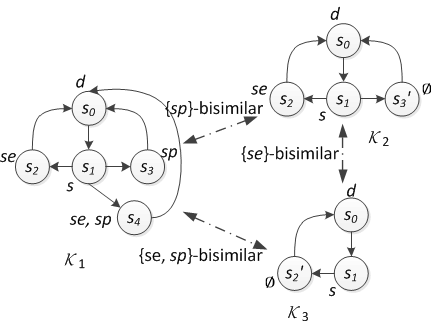
\includegraphics[width=9cm]{NVBnewCar.png}\\
		\caption{$V$-bisimulation between $\MPK$-structures}\label{v1uv2}
	\end{figure*}
\end{example}


% \begin{lemma}\label{lem:equive}
%   The relation $\lrto_V$ is an equivalence relation.
% \end{lemma}

% According to Proposition~\ref{pro:VI:prop:bisimilar:V}  and  Definition~\ref{def:VInd:bisimulation}, we have the following similar results in which indices are not taken into account.

The next proposition shows the similar properties of Proposition~\ref{prop:VI:prop:bisimilar:V} for $V$-bisimulations.

\begin{proposition}\label{prop:bisimilar:V}
	Let $i\in \{1,2\}$, $V_1,V_2\subseteq\cal A$, $s_1'$ and $s_2'$ be two states,
	$\pi_1'$ and $\pi_2'$ be two paths,
	and ${\cal K}_j=({\cal M}_j,s_j)~(j=1,2,3)$ be structures
	s.t.
	${\cal K}_1\lrto_{V_1}{\cal K}_2$ and ${\cal K}_2\lrto_{V_2}{\cal K}_3$.
	Then:
	\begin{enumerate}[(i)]
		\item ${\cal K}_1\lrto_{V_1\cup V_2}{\cal K}_3$;
		\item If $V_1 \subseteq V_2$ then ${\cal K}_1 \lrto_{V_2} {\cal K}_2$;
		\item $s_1'\lrto_{V_i}s_2'~(i=1,2)$ implies $s_1'\lrto_{V_1\cup V_2}s_2'$;
		\item $\pi_1'\lrto_{V_i}\pi_2'~(i=1,2)$ implies $\pi_1'\lrto_{V_1\cup V_2}\pi_2'$;
		\item for each path $\pi_{s_1}$ of $\Hm_1$ there is a path $\pi_{s_2}$  of $\Hm_2$ s.t. $\pi_{s_1} \lrto_{V_1} \pi_{s_2}$, and vice versa.
	\end{enumerate}
\end{proposition}


In Proposition~\ref{prop:bisimilar:V}, properties $(i)$ to $(iii)$ are the standard properties for $V$-bisimulation.
Property $(iv)$ shows that if a  structure is $V_1$ and $V_2$-bisimilar with the other two structures, respectively, then those two structures are $V_1 \cup V_2$-bisimilar. For an example, see Figure~\ref{v1uv2}. This property is crucial for forgetting.
%since it lays the foundation of forgetting atoms in $V$ one by one.
And last, $(v)$ says that if two  structures are  $V_1$-bisimilar, then they are $V_2$-bisimilar for any $V_2$ with $V_1\subseteq V_2 \subseteq \Ha$.






Intuitively, if two structures are $V$-bisimilar, then they satisfy the same \CTL\
formula $\varphi$ that does not contain any atoms in $V$, i.e., $\IR(\varphi, V)$. This idea has been formalized and shown in the following theorem.

\begin{theorem}\label{thm:V-bisimulation:EQ}
	Let $V\subseteq\cal A$, ${\cal K}_i~(i=1,2)$ be two structures s.t.
	${\cal K}_1\lrto_V{\cal K}_2$ and $\phi$ be a \CTL\ formula with $\IR(\phi,V)$. Then
	${\cal K}_1\models\phi$ if and only if ${\cal K}_2\models\phi$.
\end{theorem}

Please note that the formula $\phi$ in the above theorem must have no index. Otherwise, the index function
in ${\cal I}$-structures may affect the satisfiability. For instance, let $\phi=\EXIST_{\tuple{1}}\NEXT p$,
${\cal K}=(\Hm,s)$ and $\Hm=(S,R,L,[\_],s_0)$ where $S=\{s_0,s_1\}$, $L(s_0)=\emptyset$, $L(s_1)=\{p\}$,
$R=\{(s_0,s_1),(s_0,s_0),(s_1,s_1), (s_1,s_0)\}$ and $[1]=\{(s_0,s_1), (s_1,s_1)\}$. It is clear ${\cal K}\models\phi$.
Let ${\cal K}'=(\Hm',s)$ and $\Hm'=(S,R,L,[\_]',s_0)$ with $[1]'=\{(s_0,s_0),(s_1,s_1)\}$.
It is evident ${\cal K}\lrto_{\{q\}}{\cal K}'$ and $\IR(\phi,\{q\})$. However, ${\cal K}'\not\models\phi$.


It is not difficult to check that, for the formulas  $\varphi_1= d \wedge \EXIST\FUTURE se \wedge \ALL\GLOBAL(se \rto \ALL\NEXT d)$
and $\varphi_2= d \wedge \ALL \NEXT se$, they are  $\{sp\}$-irrelevant and the structures ${\cal K}_1$ and ${\cal K}_2$ in Figure~\ref{v1uv2} satisfy $\varphi_1$, but not $\varphi_2$.
%
%Below, we illustrate this idea over an example.
%
%\begin{example}[Continued from Example~\ref{ex:2}]\label{ex:3}
%	Let $\varphi_1= d \wedge \EXIST\FUTURE se \wedge \ALL\GLOBAL(se \rto \ALL\NEXT d)$ and $\varphi_2= d \wedge \ALL \NEXT se$.  They are  $\{sp\}$-irrelevant. One can see that ${\cal K}_1$ and ${\cal K}_2$ in Figure~\ref{v1uv2} satisfy $\varphi_1$, but not $\varphi_2$.
%\end{example}

\begin{definition}[bisimular equivalence]\label{def:bisimular:equivalene}
Let $V\subseteq {\cal A}$. Two formulas $\varphi$ and $\psi$ are {\em $V$-bisimularly equivalent}, written $\varphi\equiv_V\psi$,
whenever, for every ${\cal K}\models \varphi$, there exists ${\cal K}'\models\psi$ such that ${\cal K}\lrto_V{\cal K}'$, and
vice versa.
\end{definition}

The below lemma follows easily from Definitions~\ref{def:VInd:bisimulation} and \ref{def:bisimular:equivalene}, and Proposition~\ref{prop:bisimilar:V}.
\begin{lemma}
 For any $V\subseteq\cal A$,  $\lrto_V$  and $\equiv_V$ are equivalent relations.
\end{lemma}
\begin{proof}
  The relation $\lrto_V$ is transitive by (i) of Proposition~\ref{prop:bisimilar:V}. It is obviously reflexive and symmetric. Thus, it is an equivalent relation.

  The relation  $\equiv_V$ is obviously reflexive and symmetric.
  Suppose that $\varphi\equiv_V\psi$ and $\psi\equiv_V\xi$. It follows that, for any ${\cal K}\models\varphi$,
  there exists ${\cal K}'\models\psi$ \st ${\cal K}'\lrto_V{\cal K}$ by  $\varphi\equiv_V\psi$, and there exists ${\cal K}''\models\xi$ \st
  ${\cal K}'\lrto_V{\cal K}''$ by $\psi\equiv_V\xi$. Since $\lrto_V$ is an equivalent relation, we have
  ${\cal K}\lrto_V{\cal K}''$. Similarly, for any ${\cal K}''\models\xi$, there exists ${\cal K}\models \varphi$
  \st ${\cal K}''\lrto_V{\cal K}$. It implies the transitivity of $\equiv_V$. Thus, it is an equivalent relation.
\end{proof} p

The bellow corollary follows from the above definition and Proposition~\ref{prop:bisimilar:V}.
\begin{corollary}
  Let $V,V_1,V_2$ be subsets of $\cal A$, $\varphi$ and $\psi$ be formulas.
  \begin{enumerate}[(i)]
    \item If $\varphi\equiv\psi$ then $\varphi\equiv_V\psi$.
    \item If both $\varphi$ and $\psi$ contain no index and $\varphi\equiv_\emptyset\psi$ then $\varphi\equiv\psi$.
    \item If $\varphi\equiv_{V_i}\psi~(i=1,2)$ then $\varphi\equiv_{V_1\cup V_2}\psi$.
    \item If $\varphi\equiv_{V_1}\psi$ and $V_1\subseteq V_2$ then $\varphi\equiv_{V_2}\psi$.
  \end{enumerate}
\end{corollary}

Please note that the condition  ``$\varphi$ and $\psi$ contain no index'' of (ii) is necessary. Otherwise let $\varphi=\EXIST_{\tuple{1}}\NEXT p $ and
$\psi=\EXIST_{\tuple{2}}\NEXT p $. One can verify $\varphi\equiv_\emptyset \psi$, but $\varphi\not\equiv\psi$.

%%%Note that the bisimular relation $\lrto_V$ is transitive by (i) of Proposition~\ref{prop:bisimilar:V} an equivalent relation


\begin{proposition}\label{prop:transform:V:EQ}
  Let $\varphi$ be a \CTL\ formula. Then $\varphi\equiv_UT_\varphi$ where $T_\varphi=\CTLsnf(\varphi)$ and
  $U=\Var(T_\varphi)-\Var(\varphi)$.
\end{proposition}

\subsection{Semantic Forgetting}
%Resolution:这种情形下得到的结果包括新引入的命题(没有约束,下文接着介绍封闭的情形。这样就更连贯了)
%CTL下的forgetting是不封闭的,在下节中将讨论其在bounded CTL下是封闭的。
In this subsection, we present the notion of forgetting in \CTL\ and investigate its semantic properties. Let us start with the formal definition.
\begin{definition}[\CTL-Forgetting]\label{def:V:forgetting}
	Let $V\subseteq\cal A$ and $\phi$ be a \CTL\ formula.
	A \CTL\ formula $\psi$ with $\Var(\psi)\cap V=\emptyset$
	is a {\em result of forgetting $V$ from} $\phi$, if
	\begin{equation*}
		\Mod(\psi)=\{{\cal K} \mid \exists {\cal K}'\in\Mod(\phi)\ \text{ \st }\ {\cal K}'\lrto_V{\cal K}\}.
	\end{equation*}
\end{definition}


According to the above definition,  if both formulas $\psi$ and $\psi'$ are results of forgetting $V$ from $\phi$, then
$\Mod(\psi)=\Mod(\psi')$. In this sense, the result of  forgetting $V$ from $\phi$ is unique up to equivalence whenever the result exists.
In this case we denote the forgetting result by $\CTLforget(\phi,V)$, which means that the result of forgetting $V$ from $\phi$
is expressible in the logic \CTL, unless explicitly stated otherwise.
In what follows, %when there is only one element in the collection, we also use this element to replace this collection, e.g.,
we write $\CTLforget(\phi,\{p\})$ as $\CTLforget(\phi,p)$ for convenience.

Please note  that the above definition does not assert the existence of the forgetting result.
In fact, there are \CTL\ formulas whose forgetting results do not exist. %
%This property corresponds to the {\em uniform interpolation} (or {\em Craig interpolation}) property.
%Formally, a logic ${\cal L}$ has {\em uniform interpolation} (or {\em Craig interpolation}) property
%if, for any formulas $\varphi$ and $\psi$ with $\varphi\vdash_{\cal L} \psi$, there exists a formula
%$\xi$ such that $\varphi\vdash_{\cal L}\xi$, $\xi\vdash_{\cal L}\psi$ and $\Var(\xi)\subseteq \Var(\varphi)\cap \Var(\psi)$.
%It is well-known that the uniform interpolation property fails for the temporal logics LTL, \CTL\  and $\CTL^*$~\cite{Maksimova:JANCL:1991,DAgostino:synthese:2008}.
%This is different from the bounded \CTL\ which has only finite signature and finite states.
%The bounded \CTL\ has finite model property, which implies that every finite model can be characterized by a \CTL\ formula.
%This follows that the forgetting result for bounded \CTL\ always exists~\cite{renyansfirstpaper}.
%
%In fact, the below example shows this possibility.
For instance,  let $p$ and $x$ be two distinct propositions and $\varphi(p,x)$\footnote{$\varphi(p,x)$ means the formula $\varphi$ with $\Var(\varphi)=\{p,x\}$.}
%\ \varphi_1(p,x) \wedge \varphi_2(x) \wedge \varphi_3(p,x) \wedge \varphi_4(p,x) \wedge \varphi_5(p)$ obtained from
be the conjunction of the following formulas~\cite{Maksimova:JANCL:1991}:
%\begin{align*}
%     \varphi_1(p,x) =\ &\ALL\GLOBAL(\neg x \wedge \neg \ALL \GLOBAL p \rto \neg \ALL \NEXT \neg x), \\
%     \varphi_2(x) =\ & \ALL\GLOBAL(\neg \ALL\NEXT \neg x \rto \ALL \NEXT x),\\
%     \varphi_3(p,x) =\ & \ALL\GLOBAL(\ALL\NEXT x \rto \neg x \wedge \neg \ALL \GLOBAL p),\\
%     \varphi_4(p,x) =\ & \ALL\GLOBAL(x \rto \neg \ALL\GLOBAL p),\\
%     \varphi_5(p) =\ & \ALL\GLOBAL(\ALL \FUTURE \ALL \GLOBAL p).
%\end{align*}
\begin{align*}
      &\ALL\GLOBAL(\neg x \wedge \neg \ALL \GLOBAL p \rto \neg \ALL \NEXT \neg x),
      \qquad \ALL\GLOBAL(\neg \ALL\NEXT \neg x \rto \ALL \NEXT x),\\
      & \ALL\GLOBAL(\ALL\NEXT x \rto \neg x \wedge \neg \ALL \GLOBAL p),
      \qquad \ALL\GLOBAL(x \rto \neg \ALL\GLOBAL p),
      \qquad \ALL\GLOBAL(\ALL \FUTURE \ALL \GLOBAL p).
\end{align*}
\citeauthor{Maksimova:JANCL:1991} showed that $\varphi(p,x)\land \varphi(p,y)\models x\lrto y$ and there is
no \CTL\ formula $\psi$ with $\Var(\psi)=\{p\}$ such that
$\varphi(p,x)\models x\lrto \psi$, viz., the logic \CTL\ has no explicitly definability ({\em Beth property}). This implies the below
assertion.
\begin{proposition}
  $\CTLforget(x\land \varphi(p,x), \{x\})$ is not expressible in \CTL.
\end{proposition}
\begin{proof}
Let $\psi(p)=\CTLforget(x\land \varphi(p,x), \{x\})$ be a \CTL\ formula.
We have \\
$\varphi(p,x)\land \varphi(p,y)\vdash x\lrto y$\\
$\Rto$ $\varphi(p,x)\land x \vdash \varphi(p,y)\rto y$\\
$\Rto$ $\varphi(p,x)\land x\vdash \psi(p)$ and $\psi(p)\vdash \varphi(p,y)\rto p(y)$ (Theorem~\ref{thm:close})\\
$\Rto$ $\varphi(p,x)\vdash x\rto\psi(p)$, and $\varphi(p,y)\vdash \psi(p)\rto p(y)$ which implies $\varphi(p,x)\vdash \psi(p)\rto p(x)$\\
$\Rto$ $\varphi(p,x)\vdash x\lrto \psi(p)$, a contradiction.
\end{proof}

In fact, the existence (or expressibility) of forgetting results correspond to the {\em uniform interpolation} (or {\em Craig interpolation}) property.
Formally, a logic ${\cal L}$ has {uniform interpolation} (or {Craig interpolation}) property
if, for any formulas $\varphi$ and $\psi$ with $\varphi\vdash_{\cal L} \psi$, there exists a formula
$\xi$ such that $\varphi\vdash_{\cal L}\xi$, $\xi\vdash_{\cal L}\psi$ and $\Var(\xi)\subseteq \Var(\varphi)\cap \Var(\psi)$.
It is well-known that the uniform interpolation property fails for the temporal logics LTL, \CTL\  and $\CTL^*$~\cite{Maksimova:JANCL:1991,DAgostino:synthese:2008}.
This is different from the bounded \CTL\ which has only finite signature and finite states.
The bounded \CTL\ has finite model property, which implies that every finite model can be characterized by a \CTL\ formula.
This follows that the forgetting result for bounded \CTL\ always exists~\cite{renyansfirstpaper}.

% At this point, it is important to emphasize that, the notion of forgetting  we have defined for \CTL\ respects the forgetting defined for PL~\cite{lin1994forget}. To see this, assume that $\varphi$ is a PL formula and $p\in \Ha$, then $\Forget(\varphi, \{p\})$ is a result of forgetting $p$ from $\varphi$; that is, $\Forget(\varphi,\{p\})\equiv \varphi[p/\bot] \vee \varphi[p/\top]$.
% That way, given a set $V\subseteq \Ha$, one can recursively define $\Forget(\varphi, V\cup \{p\}) = \Forget(\Forget(\varphi, \{p\}),V)$, where $\Forget(\varphi, \emptyset) = \varphi$. Using this insight, the following result shows that the classical notion of forgetting (for PL ~\cite{lin1994forget}) is a special case of forgetting in \CTL.
The  next proposition shows that, for propositional formulas, the above \CTL-forgetting agrees with the classical forgetting~\cite{lin1994forget}.

\begin{theorem}\label{thm:PL:CTL}
	Let $\varphi$ be a formula of propositional logic and $V\subseteq \Ha$, then
	\[
	\CTLforget(\varphi, V) \equiv \Forget(\varphi, V).
	\]
\end{theorem}


It is noteworthy  that the $V$-irrelevant is of crucial importance for computing SNC and WSC. Consider the $\psi=\varphi\wedge (q\lrto \alpha)$. If $\IR(\varphi \wedge \alpha, \{q\})$, then the result of forgetting $q$ from $\psi$ is $\varphi$. This property is described in the following lemma, and as we will later see in Section~6, it will become important (in reducing the SNC (WSC) of any \CTL\ formula to the one of a proposition).

\begin{lemma}\label{lem:KF:eq}
	Let $\varphi$ and $\alpha$ be two \CTL\ formulas and $q\not \in
	(\Var(\varphi) \cup \Var(\alpha))$. Then
	$\CTLforget(\varphi \wedge (q\lrto\alpha), q)\equiv \varphi$.
\end{lemma}


In what follows, we list other properties of the forgetting operator. According to the definition of forgetting, the set of atoms to be forgotten should be forgotten as a whole.
The following property guarantees that this can be achieved modularly by applying forgetting one by one to the atoms to be forgotten.
\begin{proposition}[Modularity]\label{disTF}
	Given a \CTL\ formula $\varphi$, a set $V$ of atoms, and an atom $p$ s.t.  $p \notin V$, then
	\[
	\CTLforget(\varphi, \{p\} \cup V) \equiv \CTLforget(\CTLforget(\varphi, p), V).
	\]
\end{proposition}

The next property follows from the above proposition.

\begin{corollary}[Commutativity]\label{disTFV}
	Let $\varphi$ be a \CTL\ formula and $V_i\subseteq{\cal A}~(i=1,2)$. Then:
	\[
	\CTLforget(\varphi, V_1 \cup V_2) \equiv \CTLforget(\CTLforget(\varphi, V_1), V_2).
	\]
\end{corollary}


The following properties show that the forgetting respects the basic semantic notions of logic. % They hold in both   propositional logic and modal logic S5~\cite{Yan:AIJ:2009}.
Below we show that they are also satisfied in our notion forgetting in \CTL.
\begin{proposition}\label{pro:ctl:forget:1}
	Let $\varphi$, $\varphi_i$, $\psi_i$ ($i=1,2$) be formulas in \CTL\ and $V\subseteq \Ha$. We have
	\begin{enumerate}[(i)]
		\item $\CTLforget(\varphi, V)$ is satisfiable iff $\varphi$ is;
		\item If $\varphi_1 \equiv \varphi_2$, then $\CTLforget(\varphi_1, V) \equiv \CTLforget(\varphi_2, V)$;
		\item If $\varphi_1 \models \varphi_2$, then $\CTLforget(\varphi_1, V) \models \CTLforget(\varphi_2, V)$;
		\item $\CTLforget(\psi_1 \vee \psi_2, V) \equiv \CTLforget(\psi_1, V) \vee \CTLforget(\psi_2, V)$;
		\item $\CTLforget(\psi_1 \wedge \psi_2, V) \models \CTLforget(\psi_1, V) \wedge \CTLforget(\psi_2, V)$;
        \item $\CTLforget(\psi_1 \wedge \psi_2, V) \equiv \CTLforget(\psi_1, V) \wedge  \psi_2$ if $\IR(\psi_2,V)$;
	\end{enumerate}
\end{proposition}


The next property shows that forgetting a set $V\subseteq\cal A$ from a formula with path quantifiers is equivalent to quantify the result of forgetting $V$ from the formula with the same path quantifiers.
\begin{proposition}[Homogeneity]\label{pro:ctl:forget:2}
	Let $V\subseteq\cal A$ and $\phi$ a $\CTL$ formula.% then:% and $Q\in \{\EXIST, \ALL\}$.
	\begin{enumerate}[(i)]
		\item $\CTLforget(\ALL\NEXT\phi,V)\equiv \ALL\NEXT \CTLforget(\phi,V)$.
		\item $\CTLforget(\EXIST\NEXT\phi,V)\equiv\EXIST\NEXT \CTLforget(\phi,V)$.
		\item $\CTLforget(\ALL \FUTURE\phi,V)\equiv \ALL \FUTURE \CTLforget(\phi,V)$.
		\item $\CTLforget(\EXIST\FUTURE\phi,V)\equiv\EXIST\FUTURE \CTLforget(\phi,V)$.
		\item $\CTLforget(\ALL \GLOBAL\phi,V)\equiv \ALL \GLOBAL\CTLforget(\phi,V)$.
		\item $\CTLforget(\EXIST\GLOBAL\phi,V)\equiv\EXIST\GLOBAL \CTLforget(\phi,V)$.
	\end{enumerate}
\end{proposition}
\begin{proof}
  (i) $(\Rto)$ $(\Hm,s)\models\CTLforget(\ALL\NEXT\phi,V)$\\
  $\Rto$ There is $(\Hm,s)\lrto_V(\Hm',s')$ and $(\Hm',s')\models \ALL\NEXT\phi$\\
  $\Rto$ There is $(\Hm,s)\lrto_V(\Hm',s')$, and $(\Hm',s'')\models \phi$ for every $(s',s'')\in R'$ ($R'\in\Hm'$)\\
  $\Rto$ For every $(s,s_1)\in R$, there is $(s',s'_1)\in R'$ and $(\Hm,s_1)\lrto_V(\Hm',s'_1)$, and
   $(\Hm',s'')\models \phi$ for every $(s',s'')\in R'$ ($R\in \Hm$)\\
  $\Rto$ For every $(s,s_1)\in R$, there is $(\Hm,s_1)\lrto_V(\Hm',s'_1)$ and $(\Hm',s'_1)\models\phi$\\
  $\Rto$ For every $(s,s_1)\in R$, $(\Hm,s_1)\models\CTLforget(\phi,V)$\\
  $\Rto$ $(\Hm,s)\models\ALL\NEXT\CTLforget(\phi,V)$.

  $(\Lto)$ $(\Hm,s)\models\ALL\NEXT\CTLforget(\phi,V)$\\
  $\Rto$ For every $(s,s')\in R$, $(\Hm,s')\models\CTLforget(\phi,V)$ ($R\in \Hm)$\\
  $\Rto$ For every $(s,s')\in R$, there is $(\Hm,s')\lrto_V(\Hm',s'')$ and $(\Hm',s'')\models\phi$\\
  $\Rto$ For every $i\ge 0$, there is $(\Hm,s'_i)\lrto_V(\Hm'_i,s''_i)$ and $(\Hm'_i,s''_i)\models\phi$
  where $\{s'_0,s'_1,\ldots\}=\{s'\mid (s,s')\in R\}$ and $\Hm'_i=(S'_i,R'_i,L'_i,[\_]'_i,s''_i)$ (we assume $S'_i\cap S'_j=\emptyset$ when $i\neq j$)\\
  $\Rto$ $(\Hm^*,s)\lrto_V(\Hm,s)$ and $(\Hm^*,s)\models\ALL\NEXT\phi$ where
  $\Hm^*=(S^*,R^*,L^*,[\_], s)$ and
  \begin{itemize}
    \item $S^*=\{s\}\cup\bigcup_{i\ge 0}S'_i$,
    \item $R^*=\{(s,s''_i)\mid i\ge 0\}\cup \bigcup_{i\ge 0} R'_i$,
    \item $L^*=\bigcup_{i\ge 0}L'_i$ and $L^*(s)=L(s)$ where $L\in\Hm$.
  \end{itemize}
  $\Rto$ $(\Hm,s)\models \CTLforget(\ALL\NEXT\phi,V)$.
\end{proof}

We are now in the position to investigate the forgetting postulates in \CTL.
Let $\varphi$ be a \CTL\ formula,  $V\subseteq\cal A$ and  $\varphi'$ be a result of
forgetting $V$ from $\varphi$.
The {\em forgetting postulates} are as follows:
\begin{itemize}
	\item[] (\W) Weakening: $\varphi \models \varphi'$;
	\item[] (\PP) Positive Persistence:
	for any formula $\eta$, if $\IR(\eta, V)$ and $\varphi \models \eta$ then $\varphi' \models \eta$;
	\item[] (\NgP) Negative Persistence :  for any formula $\eta$,  if $\IR(\eta, V)$ and $\varphi \not \models \eta$ then $\varphi' \not \models \eta$;
	\item[] (\textbf{IR}) Irrelevance: $\IR(\varphi', V)$.
\end{itemize}

%lets explain them here
%
Intuitively, the postulate (\W) says, forgetting weakens the original formula; the postulates  (\PP) and (\NgP)
say that forgetting result does not affect formulas that are irrelevant to forgotten atoms; the postulate (\textbf{\IR}) states that
forgetting result is irrelevant to forgotten atoms.

%It is noteworthy that they are not all orthogonal, e.g., (\NgP) is a consequence of (\W) and (\PP). Nonetheless, we prefer to list them all to outline the basic intuition behind them.



\begin{theorem}[Representation Theorem]\label{thm:close}
	%Let $\varphi$, $\varphi'$ and $\phi$ be \CTL\
	Let $\varphi$ and $\varphi'$ be \CTL\ formulas and $V \subseteq \Ha$.
	%Then t
	The following statements are equivalent:
	\begin{enumerate}[(i)]
		\item $\varphi' \equiv \CTLforget(\varphi, V)$,
		\item $\varphi'\equiv \{\phi \mid\varphi \models \phi \text{ and } \IR(\phi, V)\}$,
		\item Postulates (\W), (\PP), (\NgP) and (\textbf{IR}) hold if $\varphi,   \varphi'$ and $V$ are as in (i) and (ii).
	\end{enumerate}
\end{theorem}


\section{A Resolution-based Method for Computing Forgetting}
\label{sec:resolution}
%Resolution is a well-known technology in automated theorem proving in PL and FOL~\cite{leitsch2012resolution}. It has been used to decide the satisfiability of a formula \cite{bolotov2000clausal,zhang2014resolution} in the context of \CTL.

%In this section, we will explore how the resolution rules (in Table~\ref{tab:res}) can be used to compute forgetting in \CTL\ when it exists.%, \textcolor{red}{which is not a trivial task and indeed the contribution of this article}.

%\begin{table}[tb]%[width=.9\linewidth,cols=4,pos=h]
%	\footnotesize
%	\caption{Transformation Rules. Where $T\in \{\NEXT, \GLOBAL, \FUTURE\}$,
%		%$T'\in \{\UNTIL, \UNLESS\}$,
%		$ind$ is a new index and $Q\in \{\ALL, \EXIST_{\tuple{ind}}\}$. Besides, $q$ is an atom, $l$ is a literal, $D$ is a disjunction of literals, $p$ is a fresh atom and $\varphi$, $\varphi_1$, and $\varphi_2$ are \CTL\ formulas.}\label{tab:trans}
%	\begin{tabular}{l}
%		\toprule
%		$
%		\begin{aligned}
%			& \textbf{Trans(1)}\frac{q \rto \EXIST T \varphi}{q\rto \EXIST_{\tuple{ind}} T \varphi}; \qquad
%			\textbf{Trans(2)} \frac{q \rto \EXIST (\varphi_1 \UNTIL \varphi_2)}{q\rto \EXIST_{\tuple{ind}} (\varphi_1 \UNTIL \varphi_2)};
%			&&
%			\textbf{Trans(3)} \frac{q\rto \varphi_1 \wedge \varphi_2}{q\rto \varphi_1, q\rto \varphi_2};\\
%			&   \textbf{Trans(4)}  \frac{q\rto \varphi_1 \vee \varphi_2\ (\hbox{if $\varphi_2$ is not a disjunct})}{ q\rto \varphi_1 \vee p, p\rto \varphi_2};
%			&&\textbf{Trans(5)}  \frac{q\rto D}{\top \rto \neg q \vee D};\ \frac{q\rto \perp}{ \top \rto \neg q};\ \frac{q \rto \top}{\{\}} \\
%			&  \textbf{Trans(6)} \frac{q\rto Q\NEXT \varphi\ (\hbox{if $\varphi$ is not a disjunct})}{q\rto Q\NEXT p, p\rto \varphi};
%			&& \textbf{Trans(7)} \frac{q\rto Q\FUTURE \varphi\ (\hbox{if $\varphi$ is not a literal})}{q\rto Q\FUTURE p, p\rto \varphi}; \\
%			&  \textbf{Trans(8)} \frac{q\rto Q(\varphi_1 \UNTIL \varphi_2) \  (\hbox{if $\varphi_2$ is not a literal})}{q\rto Q(\varphi_1 \UNTIL p),  p\rto \varphi_2};
%			&& \textbf{Trans(10)} \frac{q\rto Q\GLOBAL \varphi}{\ q \rto  p, p\rto \varphi,p\rto Q\NEXT p};  \\
%			& \textbf{Trans(11)} \frac{q\rto Q(\varphi \UNTIL l)}{q \rto l\vee p, p\rto \varphi, p\rto Q\NEXT(l\vee p),q\rto Q \FUTURE l};
%			&& \textbf{Trans(12)} \frac{q\rto Q(\varphi \UNLESS l)}{q \rto l\vee p, p\rto \varphi, p\rto Q\NEXT(l\vee p)}.
%		\end{aligned}
%		$\\
%		\bottomrule
%	\end{tabular}
%\end{table}

% Before that, some important notations and notions should be declared.
% We denote by $V\subseteq \Ha$, $I\subseteq \Ind$, and $V'$ with $V'\cap V =\emptyset$ the set of atoms to be forgotten, the set of indices, and the set of fresh atoms introduced in the computation, respectively.
% Moreover, let $\varphi$  be a \CTL\ formula, then $T_{\varphi}$ is the set of $\CTLsnf$ clauses obtained from $\varphi$ by applying the transformation rules (in Table~\ref{tab:trans}) and $\Hm=(S,R,L,[\_], s_0)$ (unless stated otherwise).
% Obviously, $V'= \Var(T_{\varphi}) - \Var(\varphi)$.



% In addition, we shall work with the transformation rules in Table~\ref{tab:trans} and resolution rules in Table~\ref{tab:res} mentioned above,
% which are from~\cite{zhang2014resolution}.





%\begin{table}[tb]%[width=.9\linewidth,cols=4,pos=h]
%	\footnotesize
%	\caption{Transformation Rules. Where $P$, $Q$ are conjunction of literals, $C$, $D$ are disjunction of literals and $l$ is a literal. Besides, $\Lambda=\bigvee_{i=1}^n \bigwedge_{i=1}^{m_i}P_j^i$ and $P_j^i$ are conjunction of literals for all $1\leq i\leq n$ and $1\leq j\leq m$. Note that the resolvent of both $\textbf{(ERES1)}$ and $\textbf{(ERES2)}$ can be translated into a set of $\CTLsnf$ clauses (see~\cite{zhang2014resolution}).
%	}\label{tab:res}
%	\begin{tabular}{l}
%		\toprule
%		$
%		\begin{aligned}
%			& \textbf{(SRES1)}\frac{P\rto \ALL\NEXT(C\vee l), Q\rto \ALL\NEXT(D\vee \neg l)}{P\wedge Q \rto \ALL\NEXT(C\vee D)};
%			&& \textbf{(SRES2)} \frac{P\rto \EXIST_{\tuple{ind}} \NEXT(C\vee l), Q\rto \ALL\NEXT(D\vee \neg l)}{P\wedge Q \rto \EXIST_{\tuple{ind}}\NEXT(C\vee D)};\\
%			& \textbf{(SRES3)} \frac{P\rto \EXIST_{\tuple{ind}}\NEXT(C\vee l), Q \rto \EXIST_{\tuple{ind}}\NEXT(D\vee \neg l)}{P\wedge Q\rto\EXIST_{\tuple{ind}}\NEXT(C\vee D)};
%			&&   \textbf{(SRES4)} \frac{\start \rto C\vee l, \start \rto D \vee \neg l}{\start \rto C\vee D}; \\
%			& \textbf{(SRES5)} \frac{\top \rto C\vee l, \start \rto D \vee \neg l}{\start \rto C \vee D};
%			&&  \textbf{(SRES6)} \frac{\top \rto C \vee l, Q \rto \ALL\NEXT(D \vee \neg l)}{Q\rto \ALL \NEXT(C\vee D)}; \\
%			& \textbf{(SRES7)} \frac{\top \rto C \vee l, Q \rto \EXIST_{\tuple{ind}} \NEXT(D \vee \neg l)}{Q\rto \EXIST_{\tuple{ind}}\NEXT(C\vee D)};
%			&&  \textbf{(SRES8)} \frac{\top \rto C\vee l, \top \rto D \vee \neg l}{\top \rto C \vee D};\\
%			& \textbf{(RW1)} \frac{\bigwedge_{i=1}^n m_i \rto \ALL\NEXT \perp}{\top \rto \bigvee_{i=1}^n \neg m};
%			&& \textbf{(RW2)} \frac{\bigwedge_{i=1}^n m_i \rto \EXIST_{\tuple{ind}}\NEXT \perp}{\top \rto \bigvee_{i=1}^n \neg m}; \\
%			& \textbf{(ERES1)} \frac{\Lambda \rto \EXIST_{\tuple{ind}} \NEXT \EXIST_{\tuple{ind}}\GLOBAL l, Q \rto \ALL \FUTURE \neg l}{Q \rto \ALL(\neg \Lambda \UNLESS \neg l)};
%			&& \textbf{(ERES2)} \frac{\Lambda \rto \EXIST_{\tuple{ind}} \NEXT \EXIST_{\tuple{ind}}\GLOBAL l, Q \rto \EXIST_{\tuple{ind}} \FUTURE \neg l}{Q \rto \EXIST_{\tuple{ind}}(\neg \Lambda \UNLESS \neg l)}.
%		\end{aligned}
%		$\\
%		\bottomrule
%	\end{tabular}
%\end{table}



% \begin{table*}[h]
% %\footnotesize
% \begin{center}
%     \begin{tabular}{l}
%     $
% \begin{aligned}
% & \textbf{(SRES1)}\frac{P\rto \ALL\NEXT(C\vee l), Q\rto \ALL\NEXT(D\vee \neg l)}{P\wedge Q \rto \ALL\NEXT(C\vee D)};
% && \textbf{(SRES2)} \frac{P\rto \EXIST_{\tuple{ind}} \NEXT(C\vee l), Q\rto \ALL\NEXT(D\vee \neg l)}{P\wedge Q \rto \EXIST_{\tuple{ind}}\NEXT(C\vee D)};\\
% & \textbf{(SRES3)} \frac{P\rto \EXIST_{\tuple{ind}}\NEXT(C\vee l), Q \rto \EXIST_{\tuple{ind}}\NEXT(D\vee \neg l)}{P\wedge Q\rto\EXIST_{\tuple{ind}}\NEXT(C\vee D)};
% &&   \textbf{(SRES4)} \frac{\start \rto C\vee l, \start \rto D \vee \neg l}{\start \rto C\vee D}; \\
% & \textbf{(SRES5)} \frac{\top \rto C\vee l, \start \rto D \vee \neg l}{\start \rto C \vee D};
% &&  \textbf{(SRES6)} \frac{\top \rto C \vee l, Q \rto \ALL\NEXT(D \vee \neg l)}{Q\rto \ALL \NEXT(C\vee D)}; \\
% & \textbf{(SRES7)} \frac{\top \rto C \vee l, Q \rto \EXIST_{\tuple{ind}} \NEXT(D \vee \neg l)}{Q\rto \EXIST_{\tuple{ind}}\NEXT(C\vee D)};
% &&  \textbf{(SRES8)} \frac{\top \rto C\vee l, \top \rto D \vee \neg l}{\top \rto C \vee D};\\
% & \textbf{(RW1)} \frac{\bigwedge_{i=1}^n m_i \rto \ALL\NEXT \perp}{\top \rto \bigvee_{i=1}^n \neg m};  \quad
% \textbf{(RW2)} \frac{\bigwedge_{i=1}^n m_i \rto \EXIST_{\tuple{ind}}\NEXT \perp}{\top \rto \bigvee_{i=1}^n \neg m};
% && \textbf{(ERES1)} \frac{\Lambda \rto \EXIST_{\tuple{ind}} \NEXT \EXIST_{\tuple{ind}}\GLOBAL l, Q \rto \ALL \FUTURE \neg l}{Q \rto \ALL(\neg \Lambda \UNLESS \neg l)};\\
% &  \textbf{(ERES2)} \frac{\Lambda \rto \EXIST_{\tuple{ind}} \NEXT \EXIST_{\tuple{ind}}\GLOBAL l, Q \rto \EXIST_{\tuple{ind}} \FUTURE \neg l}{Q \rto \EXIST_{\tuple{ind}}(\neg \Lambda \UNLESS \neg l)}.
% \end{aligned}
% $\\
% \end{tabular}
% \end{center}
%   where $P$, $Q$ are conjunction of literals, $C$, $D$ are disjunction of literals and $l$ is a literal. Besides, $\Lambda=\bigvee_{i=1}^n \bigwedge_{i=1}^{m_i}P_j^i$ and $P_j^i$ are conjunction of literals for all $1\leq i\leq n$ and $1\leq j\leq m$. Note that the resolvent of both $\textbf{(ERES1)}$ and $\textbf{(ERES2)}$ can be translated into a set of $\CTLsnf$ clauses (see~\cite{zhang2014resolution}).
%   %In this paper, we assume all of the results are  $\CTLsnf$ clauses.
%     \caption{Resolution Rules}\label{tab:res}
% \end{table*}
%
%
% We are now ready to introduce our resolution-method for forgetting. Algorithm~\ref{alg:compute:forgetting:by:Resolution} computes forgetting in \CTL.
In this section, we will explore how the resolution rules (in Table~\ref{tab:res}) can be used to compute forgetting in \CTL\ when it exists. The main idea  is that first, we turn the given \CTL\ formula into a set of $\CTLsnf$ clauses, and then we compute all the possible resolvents on the forgotten atoms and eliminate all the clauses containing forgotten  atoms.
Finally, we translate the remanning $\CTLsnf$ clauses  back to \CTL\ formulas.

Let $T$ be a finite set of $\CTLsnf$ clauses and $p$ an atom.   The {\em unfolding} of $T$ on $p$, written
$\Unfolding(T,p)$, is the set $T$ together with
\[\{\alpha\mid \mbox{$\alpha$ is a resolvent obtained from $T$ where the resolved literal $l\in\{p,\neg p\}$}\}.  \]
For a set $V$ of atoms, we define $\Unfolding(T,\emptyset)=T$ and $\Unfolding(T,\{p\}\cup V)=\Unfolding(\Unfolding(T,\{p\}), V)$.
Intuitively, unfolding $T$ on an atom $p$ is to do exhaustive resolution on $p$. In other words,
no more new $\CTLsnf$ clause can be generated using any of the step resolution rules {\bf SRES1-8} to resolve the literal $p$ or $\neg p$, even
after the applying of rewrite rules and eventuality resolution rules.


The next proposition shows that, for any \CTL\ formula $\varphi$,
removing the clauses mentioning atoms in $V$ from $\Unfolding(T_\varphi,V)$ remains bisimular equivalence when discarding
these atoms in $V$.
In what follows we denote $\emph{ERes}(\varphi,V) = \{\alpha\in \Unfolding(T_\varphi,V)\mid \Var(\alpha)\cap V=\emptyset\}$.
\begin{proposition}
  Let $\varphi$ be a \CTL\ formula and $V\subseteq\cal A$. Then
  $T_\varphi \equiv_U\emph{ERes}(\varphi,V)$ where  $U=\Unfolding(T_\varphi,V)-\Var(\varphi)$.
\end{proposition}


\begin{example}[Continued from Example~\ref{examp:Tran}]\label{examp:Res}
 Let $V=\{p,r\}$. Then $\Unfolding(T_\varphi, V\cup \{x,y,z\})$ consists of the following clauses, in addition to the ones in Example~\ref{examp:Tran}:
%	The resolvents, obtained by executing the resolution process on $T_{\varphi}$ of Example~\ref{examp:Tran} and $V\cup V'$, are the following clauses (in addition to the ones in Example~\ref{examp:Tran}):
	% The \textcolor{red}{resolvent} \textcolor{blue}{resolvents} of $T_{\varphi}$ obtained from Example~\ref{examp:Tran} by executing the resolution process on $T_{\varphi}$ and $V\cup V'$ are the following clauses (in addition to the ones in Example~\ref{examp:Tran}):
	\begin{align*}
		&(1)\ \start \rto r && (1,2,\textbf{SRES5})
		&&(2)\ \start \rto x \vee y && (1,4,\textbf{SRES5})\\
		% \end{align*}
		% \begin{align*}
		&(3)\ \top \rto \neg z \vee y \vee f \vee m && (3, 4, \textbf{SRES8})
		&&(4)\ y \rto \ALL\NEXT(f\vee m\vee y) && (3,8, \textbf{SRES6})\\
		&(5)\ \top \rto \neg z \vee x \vee p && (4,5, \textbf{SRES8})
		&&(6)\ \top \rto \neg z \vee x \vee q && (4,6, \textbf{SRES8})\\
		&(7)\ y \rto \ALL\NEXT(x\vee p) && (5, 8, \textbf{SRES6})
		&&(8)\ y \rto \ALL\NEXT(x\vee q) && (6, 8, \textbf{SRES6})\\
		&(9)\ \start \rto f\vee m \vee y && (3,(2), \textbf{SRES5})
		% \end{align*}
		% \begin{align*}
		&&(10)\ \start \rto x \vee p && (5,(2),\textbf{SRES5}) \\
		&(11)\ \start \rto x \vee q && (6,(2), \textbf{SRES5})
		&& (12)\ \top \rto p \vee \neg z \vee f \vee m && (5,(3), \textbf{SRES8})\\
		& (13)\ \top \rto q \vee \neg z \vee f \vee m && (6,(3), \textbf{SRES8})
		&&(14)\ y \rto \ALL\NEXT(p \vee f\vee m) && (5, (4), \textbf{SRES6})\\
		&(15)\ y \rto \ALL\NEXT(q \vee f\vee m) && (6, (4), \textbf{SRES6})
		%\end{align*}
		%\begin{align*}
		&&(16)\ \start \rto f\vee m \vee p && (5, (9), \textbf{SRES5}) \\
		&(17)\ \start \rto f\vee m \vee q && (6, (9), \textbf{SRES5})
	\end{align*}

    After removing clauses from $\Unfolding(T_\varphi, V\cup \{x,y,z\})$ that contain some atoms in $V$, we have $\emph{ERes}(\varphi,V)$
    consisting of the following clauses:
	\begin{align*}%{llll}
		&\start\rto z, \quad \start \rto f\vee m \vee q, \quad  \start \rto x \vee y, \quad \start \rto q \vee x, \quad	\start \rto f\vee m \vee y, \\
		& \top \rto f \vee m \vee \neg x, \quad		\top \rto q \vee f \vee m\vee \neg z,
            \quad  	\top \rto f \vee m \vee \neg z \vee y,\\
		& \top \rto q \vee x\vee \neg z, \quad 	\top \rto x \vee y \vee \neg z, \quad 	\top \rto q\vee\neg y , \quad z \rto \ALL \FUTURE x, \\
		& y \rto \ALL\NEXT(q \vee f\vee m), \quad  y \rto \ALL\NEXT(x\vee q), \quad y \rto \ALL \NEXT(x\vee y),\quad 	y \rto \ALL\NEXT(f\vee m\vee y).
	\end{align*}
	
    We see that  $\emph{ERes}(\varphi,V)$ have some clauses mentioning the refreshed atoms in $T_\varphi$, though
    no index is mentioned in the example.
\end{example}



%$\Gamma = \Delta\cup$ $ \Gamma'$ with

With the follow lemma, we can reduce some atoms while preserving equi-satisfiability.

\begin{lemma}[Generalised Ackermann's Lemma] \label{thm:Aclm}
 Let $x$ be an atom, $\Delta = \{\top \rto \neg x \vee C_1$, \dots, $\top \rto \neg x \vee C_n, x \rto B_1, \dots, x \rto B_m\}$
 be a set of $\CTLsnf$ clauses in which the unique occurrence of $x$ is negative,
 and $\Gamma$ be a set of $\CTLsnf$ clauses in which $x$ occurs positively.
 Then we have
 \begin{equation}\label{eq:Ackermann:lemma}
    \Gamma\cup \Delta \equiv_{\{x\}}  
    \Gamma\left[x/\bigwedge\left(\{C_i\mid 1\le i\le n\}\cup\{B_i\mid 1\le i\le m\}\right)\right].
 \end{equation}
\end{lemma}
%
In this case we define $\GAL(\Gamma\cup\Delta,\{x\})=\Gamma\left[x/\bigwedge\left(\{C_i\mid 1\le i\le n\}\cup\{B_i\mid 1\le i\le m\}\right)\right]$,
and $\GAL(\Gamma\cup\Delta,\{x\})=\Gamma\cup\Delta$ otherwise. For a set $V$ of atoms, we define
$$\GAL(\Gamma\cup\Delta,V\cup\{x\})=\GAL(\GAL(\Gamma\cup\Delta,\{x\}),V).$$
 
\begin{example}[Continued from Example~\ref{examp:Res}]\label{examp:Aclm}
   Firstly, we consider the atom $x$ and $\Delta=\{\top \rto f \vee m \vee \neg x\}$ and $\Gamma=\emph{ERes}(\varphi,V)-\Delta$.
   Any clause in $\Gamma$ that mentions $x$ is positive \wrt\ $x$. Then we have $\Gamma[x/(f \vee m)]$ consisting of the following clauses:
	\begin{align*}%{llll}
		& \start\rto z, \quad \start \rto f\vee m \vee q, \quad  \start \rto f \vee m \vee y, \\
           % \quad \start \rto q \vee f \vee m, \quad	\start \rto f\vee m \vee y, \\
		%& \top \rto q \vee f \vee m\vee \neg z,   \quad  	\top \rto f \vee m \vee \neg z \vee y,\\
		& \top \rto q \vee f \vee m \vee \neg z, \quad 	\top \rto f \vee m \vee y \vee \neg z,
        \quad \top \rto q\vee\neg y , \quad z \rto \ALL \FUTURE (f \vee m), \\
		& y \rto \ALL\NEXT(q \vee f\vee m), %\quad  y \rto \ALL\NEXT(f \vee m\vee q), %\quad y \rto \ALL \NEXT(f \vee m\vee y),
        \quad 	y \rto \ALL\NEXT(f\vee m\vee y).
	\end{align*}

    Next, we consider the atom $z$,
    $\Delta'=\{ \top \rto q \vee f \vee m \vee \neg z, \top \rto f \vee m \vee y \vee \neg z ,z \rto \ALL \FUTURE (f \vee m)\}$
    and $\Gamma'=\Gamma[x/(f \vee m)] -\Delta'$ in which the atom $z$ occurs positively. Then we have
    $\Gamma''=\Gamma'[z/ (q \vee f \vee m)\land (f \vee m \vee y)\land\ALL \FUTURE (f \vee m)]$ consisting of
 	\begin{align*}%{llll}
		& \start\rto  (q \vee f \vee m)\land (f \vee m \vee y)\land\ALL \FUTURE (f \vee m),
        \quad \start \rto f\vee m \vee q, \quad  \start \rto f \vee m \vee y,  \\
        &  \top \rto q\vee\neg y,  \quad y \rto \ALL\NEXT(q \vee f\vee m), \quad y \rto \ALL\NEXT(f\vee m\vee y).
	\end{align*}

    It is tedious but not difficult to check that $\emph{ERes}(\varphi,V)\equiv_{\{x,z\}} \Gamma''$.
    Please note that one can not apply the above process to $\Gamma''$ and the atom $y$ since $\Gamma''$  has a clause
    which is neither positive \wrt\ $y$, nor negative \wrt\ $y$.
\end{example}
 

The following lemma shows that, we can translate a set of $\CTLsnf$ clauses into a set of \CTL\ formulas while keeping equi-satisfiability.

\begin{lemma}~\label{lem:In2NI}
 Let $j\in {\cal I}$, $\psi_i,\varphi_i~(1\le i\le n)$ be \CTL\ formulas. We have
 \begin{enumerate}[(i)]
	 \item $\{\psi_i\rto \EXIST_{\tuple{j}} \NEXT \varphi_i \mid 1\le i\le n\}\equiv_\emptyset
        \{\left(\bigwedge_{i\in S}\psi_i\right)\rto \EXIST \NEXT \left(\bigwedge_{i\in S}\varphi_i\right)\mid S\subseteq\{1,\dots, n\}\}$, and

 	 \item $\{(\psi_1 \rto \EXIST_{\tuple{j}}\FUTURE \varphi_1), (\psi_2 \rto \EXIST_{\tuple{j}}\NEXT \varphi_2)\}$
    is $\emptyset$-bisimular equivalent to %$\equiv_\emptyset 
    \begin{equation}
    (\psi_1 \rto \varphi_1 \vee \EXIST \NEXT \EXIST \FUTURE \varphi_1)
    \wedge (\psi_2 \rto \EXIST \NEXT \varphi_2)
    \wedge (\psi_1 \wedge \psi_2 \rto ((\varphi_1 \wedge \EXIST \NEXT \varphi_2) \vee \EXIST \NEXT (\varphi_2 \wedge \EXIST \FUTURE \varphi_1))).
    \end{equation}
 \end{enumerate}
 \end{lemma}
  We denote the right side of $\equiv_\emptyset$ in (i) and (ii) by
  $rxi(\{\alpha_i\mid 1\le i\le n\})$ and $rfi(\{\beta_1,\alpha_2\})$, respectively, where
$\alpha_i=\psi_i\rto \EXIST_{\tuple{j}} \NEXT \varphi_i~(1\le i\le n)$ and $\beta_1=\psi_1 \rto \EXIST_{\tuple{j}}\FUTURE \varphi_1$.


We are now in the position to present the algorithm of compute \CTL\ forgetting,  Algorithm~\ref{alg:compute:forgetting:by:Resolution}.
It accepts a \CTL\ formula $\varphi$ and returns a \CTL\ theory $\Sigma$ which is bisimular equivalent to $\varphi$ when discarding the atoms 
occurring in  $\Var(\Sigma)-\Var(\varphi)\cup V$.
%
%This process is presented in detail in Algorithm~\ref{alg:compute:forgetting:by:Resolution}, i.e., input a \CTL\ formula and output a \CTL\ formula \emph{ERes}$(\varphi, V)$.
%To achieve this, the first key challenge we are confronted with is how to bridge the gap between \CTL\ \emph{and $\CTLsnf$}? (This is, in particular, necessary since there are indices for existential quantifiers in $\CTLsnf$, e.g.,  see Table~\ref{tab:trans} and Table~\ref{tab:res}).


\begin{algorithm}[tb]
	\caption{{\CTL-forget}$(\varphi, V)$}
	\label{alg:compute:forgetting:by:Resolution}
	\LinesNumbered
	\KwIn{A \CTL\ formula $\varphi$ and a set $V$ of atoms}%, and a Boolean variable ri}
	\KwOut{A conjunction of formulas}
	\lIf{$\varphi\equiv\bot$} {{\bf \Return $\bot$}\;}
	\lIf{$V=\Var(\varphi)$} {{\bf \Return  $\top$}\;}
    $T_\varphi \lto \CTLsnf(\varphi)$ \tcp*{Transforming $\varphi$ into $\CTLsnf$ clauses}
    $\Sigma\lto \Unfolding(T_\varphi,V\cup U)$ where $U=\Var(T_\varphi)-\Var(\varphi)$\tcp*{Unfolding}
    $\Sigma\lto \emph{ERes}(\Sigma,V)$ \tcp*{Removing clauses  which mention some atom in $V$}
    $\Sigma\lto \GAL(\Sigma,\Var(\Sigma)-\Var(\varphi))$ \tcp*{Reducing the remaining fresh atoms}
    \tcc{removing indexes from $\Sigma$}
    %\If{ri\tcc*{removing indexes from $\Sigma$}}{
        \ForEach{$\ALL$-sometime clause $\alpha\in\Sigma$}{
            $\Gamma\lto\emptyset$\;
            \ForEach{$\EXIST$-step clause $\beta\in\Sigma$ having the same index as $\alpha$}
            {$\Gamma\lto\Gamma\cup \{rfi(\alpha,\beta)\}$\;}            
            %Replacing it with an \CTL\ formula according to (ii) of Lemma~\ref{lem:In2NI}  
            $\Sigma\lto\Sigma\cup\Gamma -\{\alpha\}$\;
        }
        \ForEach{$\Delta\subseteq\Sigma$ \st\ $\Delta$ consists of all the clauses having the same index}{
            $\Sigma\lto \Sigma -\Delta \cup \{rxi(\Delta)\}$\;
            %Replacing the $\EXIST$-sometime clauses in $\Sigma$ with the index $i$ by \CTL\ formulas according to (i) of Lemma~\ref{lem:In2NI}
            }
    %    }
    Replacing each initial clause ``$\start\rto\varphi$'' by $\varphi$\;
    \Return $\Sigma$\;
\end{algorithm}



\begin{theorem}\label{thm:soundness:forget:algorithm}
  Let $\varphi$ be a \CTL\ formula, $V\subseteq\cal A$, $\Sigma=$\CTL-forget$(\varphi,V)$  and $U=\Var(\Sigma)-\Var(\varphi)$. Then
  \begin{enumerate}[(i)]
   \item $\Sigma\equiv_{V\cup U}\varphi$, and 
   \item $\Sigma\equiv\CTLforget(\varphi,V)$ if $U=\emptyset$.
  \end{enumerate}
\end{theorem}


\begin{example}[Continued from Example~\ref{examp:Aclm}]\label{examp:forget:algorithm}
 It is easy to see that \CTL-forget$(\varphi,\{p,r\})$ consists of the following formulas
  	\begin{align*}%{llll}
	&  (q \vee f \vee m)\land (f \vee m \vee y)\land\ALL \FUTURE (f \vee m), \quad \top \rto q\vee\neg y,  \\
    &  y \rto \ALL\NEXT(q \vee f\vee m), \quad y \rto \ALL\NEXT(f\vee m\vee y).
	\end{align*}
\end{example}


There are some sub-classes of \CTL\ formulas whose forgetting always exist.

\begin{proposition} \label{pro:fogCTL}
	Let $\varphi$ be a \CTL\ formula, which does not contain temporal operators $Pt {\cal T}$ with $Pt \in \{\ALL, \EXIST\}$ and ${\cal T} \in \{\UNTIL, \GLOBAL\}$, and for each atom $p\in V$ if $p$ and $\neg p$ appear in the same domain of temporal operator, then \CTL-forget$(\varphi,V) \equiv \CTLforget(\varphi, V)$.
\end{proposition}

% \begin{algorithm}[ht]
% \caption{\emph{ERes}$(\varphi, V)$}
% \label{alg:compute:forgetting:by:Resolution}
% \textbf{Input}: A \CTL\ formula $\varphi$ and a set $V$ of atoms\\
% \textbf{Output}: A conjunction of formulas
% \begin{algorithmic}[1] %[1] enables line numbers
% \STATE \textbf{if} $\varphi$ is UNSAT \textbf{then return} $\bot$;
% \STATE \textbf{if} $V=\Var(\varphi)$ \textbf{then return} $\top$;
% \STATE $T_{\varphi}, V' \lto \emph{Transform}(\varphi)$;
% \STATE $Res \lto \emph{Resolution}(T_{\varphi}, V\cup V')$ ;
% \STATE $\emph{RemA} \lto \emph{Removing\_atoms}(Res, V)$ ;
% \STATE $\NI \lto \emph{Removing\_index}(\emph{RemA})$ ; %Remove the index and start
% \STATE \textbf{return} $\bigwedge_{\psi \in \NI_{\CTL}} \psi$;
% \end{algorithmic}
% \end{algorithm}

%
%Let $\Hm=(S,R,L,[\_],s_0)$ and $\Hm'=(S',R',L',[\_],s_0')$. We can now describe the two (sets of) formulas are logically equivalent on a tuple $\tuple{V'', I}$, i.e., their models are $\tuple{V'', I}$-bisimilar with each other, in which $V''\subseteq \Ha$ and $I \subseteq \Ind$. Formally:
%\begin{definition}\label{def:vIEqu}
%	Let $T_i$ with $i \in \{1, 2\}$ be two (sets of) formulas, $I \subseteq \Ind$ and $V''\subseteq \Ha$. We say $T_1$ and $T_2$ are logically equivalent on tuple $\tuple{V'', I}$, denoted as $T_1\equiv_{\tuple{V'', I}} T_2$, if:
%	\begin{itemize}
%		\item for every $(\Hm,s_0) \in \Mod(T_1)$, there is a model $(\Hm', s_0')$ of $T_2$ s.t.  $(\Hm, s_0) \lrto_{\tuple{V'', I}} (\Hm', s_0')$, and
%		\item for every $(\Hm,s_0) \in \Mod(T_2)$, there is a model $(\Hm', s_0')$ of $T_1$ s.t. $(\Hm, s_0) \lrto_{\tuple{V'', I}} (\Hm', s_0')$.
%	\end{itemize}
%	% \begin{enumerate}[(i)]
%	%     \item for every $(\Hm,s_0) \in \Mod(T_1)$, there is a model $(\Hm', s_0')$ of $T_2$ such that $(\Hm, s_0) \lrto_{\tuple{V'', I}} (\Hm', s_0')$, and
%	%     \item for every $(\Hm,s_0) \in \Mod(T_2)$, there is a model $(\Hm', s_0')$ of $T_1$ such that $(\Hm, s_0) \lrto_{\tuple{V'', I}} (\Hm', s_0')$.
%	% \end{enumerate}
%\end{definition}
%
%Another key challenge one has to confront is  the \emph{elimination of the irrelevant atoms (from both those we want to forget and those that introduced by these rules)} which has no straightforward solution.
%To overcome this problem, we shall  eventually introduce a new \emph{elimination} process, i.e., the \emph{Removing\_atoms} process, and a generalised Ackermann’s lemma.
%
%
%In the following, we will show that \emph{ERes}$(\varphi, V) \equiv_{\tuple{V',\emptyset}} \CTLforget(\varphi, V)$.
%To achieve this, we elaborate on each process in Algorithm~\ref{alg:compute:forgetting:by:Resolution} and give a running example of how to use the algorithm to calculate forgetting.
%%To achieve this, each process will be \textcolor{red}{introduced} detailly, and a running example will be given to show how to compute forgetting using our algorithm.
%
%\subsection{The Transformation Process}
%The \emph{transformation process}, denoted as $\emph{Transform}(\varphi)$, is presented  in  detail  in Algorithm~\ref{alg:compute:trans}.
%It takes a \CTL\ formula $\varphi$ in and outputs a set $T_{\varphi}$ of $\CTLsnf$ clauses, a set $V'$ of fresh atoms, and a set $I$ of indices using  the transformation rules in Table~\ref{tab:trans} on $T_{\varphi}$ until each formula in $T_{\varphi}$ is a $\CTLsnf$ clause.
%In which $T_{\varphi}$ is initialized with $\{\ALL \GLOBAL(\start \rto p), \ALL \GLOBAL(p \rto \simp(\nnf(\varphi)))\}$~\footnote{The function $\nnf$ transforms a \CTL\ formula into a negation normal form (hence nnf), i.e., negative operations only occur before atoms, and $\simp$ is a function that uses the simplification rules in~\cite{zhang2014resolution} to simplify the $\top$ and $\bot$ appearing in the formula.}, where $p$ is a fresh atom.
%It is worth noting that throughout the transformation, formulas are kept in negation normal form (nnf).
%
%Moreover, the ``$Trans(\psi)$" in Algorithm~\ref{alg:compute:trans} means using one of the rules in Table~\ref{tab:trans} on $\psi$ and returning the result of the rule (and also the fresh atom and the index, if any). Take ``\textbf{Trans(6)}" as an example with $\psi = q \rto \ALL \NEXT \phi$. If $\phi$ is not a classical clause, then using \textbf{Trans(6)} to $\psi$ results in the set $\{q \rto \ALL \NEXT q', q' \rto \phi\}$ which introduces the fresh atom $q'$ but without fresh index.
%
%The following proposition shows that the \CTL\ formula $\varphi$ and its corresponding set $T_{\varphi}$ of $\CTLsnf$ clauses are logically equivalent on $\tuple{V', I}$.
%%
%%\begin{algorithm}[tb]
%%	\caption{\emph{Transform}$(\varphi)$}
%%	\label{alg:compute:trans}
%%	\LinesNumbered
%%	\KwIn{A \CTL\ formula $\varphi$}
%%	\KwOut{A set $T_{\varphi}$ of $\CTLsnf$ clauses, a set $V'$ of atoms, and a set $I$ of indices  }
%%	$T_{\varphi}\lto \{\ALL \GLOBAL(\start \rto p), \ALL \GLOBAL(p \rto \simp(\nnf(\varphi)))\}$ where
%%	$p\in {\cal A}-var(\varphi)$\;
%%	$V'\lto \{p\}$ \;
%%	$I\lto \emptyset$\;
%%	\While{$\exists \psi \in T_{\varphi}$ s.t. $\psi$ is not a $\CTLsnf$ clause}  {
%%         $T_{\varphi} \lto T_{\varphi}-\{\psi\}$  \;
%%         $T_{\varphi} \lto Trans(\psi) \cup T_{\varphi}$\;
%%         \lIf{$Trans(\psi)$ introduces a fresh atom $q$}{$V'\lto V' \cup \{q\}$}
%%
%%         \lIf{$Trans(\psi)$ introduces a fresh index $ind$}{$I\lto I \cup \{ind\}$}
%%         }
%%	\Return ($T_{\varphi}, V', I$)\;
%%\end{algorithm}
%
%
%\begin{proposition}\label{pro:TranE}
%	Let $\varphi$ be a \CTL\ formula and $(T_{\varphi}, V',I)=$Transform$(\varphi)$.  $\varphi \equiv_{\tuple{V', I}} T_{\varphi}$.
%\end{proposition}
%
%This shows that any \CTL\ formula $\varphi$ is only different with $T_{\varphi}$ on set $V'$ of atoms and set $I$ of indices. Let us take a look at it in our running example.
%
%%
%%\begin{example}[Running example]
%%\label{examp:Tran}
%%	Let $\varphi=\ALL((p\wedge q) \UNTIL (f\vee m)) \wedge r$ be a formula and $V=\{p,r\}$.
%%	As the first step, \emph{Transform}$(\varphi)$  will yield  the result $T_{\varphi}$, which can be listed as follows:\\
%%	% \begin{align*}
%%	% & 1. \start\rto z && 2. \top \rto \neg z \vee r && 3.\top \rto \neg x\vee f \vee m\\
%%	% & 4. \top \rto \neg z \vee x \vee y && 5.\top \rto \neg y \vee p && 6.\top \rto \neg y \vee q\\
%%	% & 7. z \rto \ALL \FUTURE x && 8. y \rto \ALL \NEXT(x\vee y).
%%	% \end{align*}
%%	$
%%	\begin{array}{llll}
%%		1. \start\rto z & 2. \top \rto \neg z \vee r \qquad & 3.\top \rto \neg x\vee f \vee m  & 4. \top \rto \neg z \vee x \vee y \\
%%		5.\top \rto \neg y \vee p &  6.\top \rto \neg y \vee q &
%%		7. z \rto \ALL \FUTURE x & 8. y \rto \ALL \NEXT(x\vee y),\\
%%	\end{array}
%%	$\\
%%	with the set $V'=\{x, y,z, w\}$ of new atoms introduced in this process, in which $w$ is a new atom related to $z \rto \ALL \FUTURE x$~\footnote{Note that we always generate a new atom $w$ for each $Q$-sometime clause with $Q\in \{\EXIST, \ALL\}$ when this clause is produced during the transformation process.}. %~\cite{zhang2014resolution}.
%%	% Besides, the set of new atoms introduced in this process is $V'=\{x, y,z, w\}$ in which $w$ is a new atom related to $z \rto \ALL \FUTURE x$~\footnote{Note that we always generate a new atom for each $T$-sometime clause with $T\in \{\EXIST, \ALL\}$ when this clause is produced during the transform process.}. %~\cite{zhang2014resolution}.
%%\end{example}
%
%
%\subsection{The Resolution Process}
%The \emph{resolution process}, i.e., $Resolution(T_{\varphi}, V \cup V')$ (with $(T_{\varphi}, V',I)=$Transform$(\varphi)$), will be executed after the transformation process and return a set of $\CTLsnf$ clauses.
%The exhaustive \emph{resolution} of $T_{\varphi}$ on a set $V''$ of atoms
%%, represented  by the function $\emph{Resolution}(T_{\varphi}, V'')$,
%is a sequence $T_0=T_{\varphi}, T_1, T_2$, $\dots$, $T_n=Res$ of sets of $\CTLsnf$ clauses s.t.  $T_{i+1} = T_i \cup R_i$ for all $0\leq i < n$ and no new clauses in $Res$ can be derived by further application of resolution rules (or a
%contradiction is derived, i.e., there is $\start\rto \perp\in T_i$ or $\top\rto \perp\in T_i$ for some $i$, in this case we can check that $\CTLforget(\varphi, V) \equiv \bot$ for any $V$),
%where $R_i$ is a set of clauses obtained as the resolvents of using a resolution rule to premises in $T_i$ and an atom in $V''$.
%Note that all $T_i$ (where $0 \leq i \leq n$) are sets of $\CTLsnf$ clauses.
%%For convenience, let $V''= V \cup V'$,
%To express the $T_{\varphi}$ explicitly, we will use $\emph{Resolution}(T_{\varphi}, V'')$ to denote the $Res$.
%Then, we have the following result.
%\begin{proposition}\label{pro:ResE}
%	Let $\varphi$ be a \CTL\ formula,
%	then $T_{\varphi} \equiv_{\tuple{V\cup V', \emptyset}} Resolution(T_{\varphi}, V \cup V')$.
%\end{proposition}
%% \begin{proof}[Proof sketch]
%% It is apparent that $Res \models T_{\varphi}$ science $T_{\varphi} \subseteq Res$.
%% The other direction can be obtained by inducting on the Resolution rules in Table~\ref{tab:res}.
%% \end{proof}
%
%Prop.~\ref{pro:ResE} and Prop.~\ref{pro:TranE}  imply that $\varphi$ $\equiv_{\tuple{V'', I}}$ $Resolution(T_{\varphi}, V'')$, where $V''= V \cup V'$. That is, for each \CTL\ formula $\psi$, $\IR(\psi, V'')$ implies $\varphi \models \psi$ iff $Resolution(T_{\varphi}, V'') \models \psi$.
%
%%\begin{example}[Continued from Example~\ref{examp:Tran}]\label{examp:Res}
%%	The resolvents, obtained by executing the resolution process on $T_{\varphi}$ of Example~\ref{examp:Tran} and $V\cup V'$, are the following clauses (in addition to the ones in Example~\ref{examp:Tran}):
%%	% The \textcolor{red}{resolvent} \textcolor{blue}{resolvents} of $T_{\varphi}$ obtained from Example~\ref{examp:Tran} by executing the resolution process on $T_{\varphi}$ and $V\cup V'$ are the following clauses (in addition to the ones in Example~\ref{examp:Tran}):
%%	\begin{align*}
%%		&(1)\ \start \rto r && (1,2,\textbf{SRES5})
%%		&&(2)\ \start \rto x \vee y && (1,4,\textbf{SRES5})\\
%%		% \end{align*}
%%		% \begin{align*}
%%		&(3)\ \top \rto \neg z \vee y \vee f \vee m && (3, 4, \textbf{SRES8})
%%		&&(4)\ y \rto \ALL\NEXT(f\vee m\vee y) && (3,8, \textbf{SRES6})\\
%%		&(5)\ \top \rto \neg z \vee x \vee p && (4,5, \textbf{SRES8})
%%		&&(6)\ \top \rto \neg z \vee x \vee q && (4,6, \textbf{SRES8})\\
%%		&(7)\ y \rto \ALL\NEXT(x\vee p) && (5, 8, \textbf{SRES6})
%%		&&(8)\ y \rto \ALL\NEXT(x\vee q) && (6, 8, \textbf{SRES6})\\
%%		&(9)\ \start \rto f\vee m \vee y && (3,(2), \textbf{SRES5})
%%		% \end{align*}
%%		% \begin{align*}
%%		&&(10)\ \start \rto x \vee p && (5,(2),\textbf{SRES5}) \\
%%		&(11)\ \start \rto x \vee q && (6,(2), \textbf{SRES5})
%%		&& (12)\ \top \rto p \vee \neg z \vee f \vee m && (5,(3), \textbf{SRES8})\\
%%		& (13)\ \top \rto q \vee \neg z \vee f \vee m && (6,(3), \textbf{SRES8})
%%		&&(14)\ y \rto \ALL\NEXT(p \vee f\vee m) && (5, (4), \textbf{SRES6})\\
%%		&(15)\ y \rto \ALL\NEXT(q \vee f\vee m) && (6, (4), \textbf{SRES6})
%%		%\end{align*}
%%		%\begin{align*}
%%		&&(16)\ \start \rto f\vee m \vee p && (5, (9), \textbf{SRES5}) \\
%%		&(17)\ \start \rto f\vee m \vee q && (6, (9), \textbf{SRES5})
%%	\end{align*}
%%\end{example}
%
%% It is easy to see that there are new atoms and indexes in the $Res$. In this case, it is needed to eliminate those new atoms and indexes to obtain the result of forgetting $V$ from $\varphi$.
%
%\subsection{The Elimination Process}
%Intuitively, the $Removing\_atoms$ process aims to remove those $\CTLsnf$ clauses which contain at least one of the atoms in $V$.
%% That is, for each $\CTLsnf$ clause $C$ and set of atoms $V$, if $\Var(C) \cap V \not = \emptyset$ then Removing\_atoms$(C, V)$ is true, else it is $C$ itself.
%That is, for each $\CTLsnf$ clause $C$ and set of atoms $V$, we have:
%\[Removing\_atoms(C, V) \equiv
%\left\{
%\begin{array}{ll}
%	 \top, \qquad \hbox{$\Var(C) \cap V \not = \emptyset$;} \\
%	C,  \qquad  \hbox{otherwise.}
%\end{array}
%\right.
%\]
%Moreover,  For any set $\Pi$ of formulas, we define that
%\[Removing\_atoms(\Pi, V) = \{Removing\_atoms(r, V) \mid r \in \Pi\}.\]
%After this process, we can obtain a set of $\CTLsnf$ clauses \emph{RemA} that do not contain any atoms in $V$.
%We also use the process, e.g., \emph{Removing\_atoms}$(\Pi, V)$, to refer to its return value, e.g., \emph{RemA}.
%Formally, we have the following result.
%
%\begin{proposition}\label{pro:remove}
%	%Let $V''=V \cup V'$, then we have
%	$Resolution(T_{\varphi}, V \cup V') \equiv_{V \cup V'}   Removing\_atoms(Resolution(T_{\varphi}, V \cup V'), V)$.
%\end{proposition}
%More clearly, the above proposition says that this process is satisfiability preserving, i.e., it does not affect the result of $Resolution(T_{\varphi}, V \cup V')$ on $\Ha - (V \cup V')$.
%%
%%\begin{example}[Continued from Example~\ref{examp:Res}]\label{examp:remA}
%%	After removing the clauses $($in $Resolution$ $(T_{\varphi}, V'')$$)$ that include atoms in $V=\{p, r\}$, the following clauses are left:\\
%%	$
%%	\begin{array}{llll}
%%		\start\rto z, &
%%		\top \rto \neg x\vee f \vee m, &
%%		\top \rto q \vee \neg z \vee f \vee m, &
%%		y \rto \ALL \NEXT(x\vee y), \\
%%		\start \rto f\vee m \vee q,  &
%%		\top \rto \neg z \vee x \vee q, &
%%		z \rto \ALL \FUTURE x, &
%%		\top \rto \neg z \vee x \vee y, \\
%%		y \rto \ALL\NEXT(q \vee f\vee m), &
%%		\start \rto x \vee y, &
%%		y \rto \ALL\NEXT(x\vee q), &
%%		\top \rto \neg z \vee y \vee f \vee m,\\
%%		\top \rto \neg y \vee q,  &
%%		\start \rto f\vee m \vee y, &
%%		y \rto \ALL\NEXT(f\vee m\vee y), &
%%		\start \rto x \vee q.
%%	\end{array}
%%	$
%%\end{example}
%
%
%\subsection{Removal of  Indices and Start}
%One of the pivotal steps of our algorithm is removing indices and the \textbf{start} from the formulas.
%By the transformation rules in Table~\ref{tab:trans}, we know that there are no two $\EXIST$-sometime clauses that have the same index, and the resolution process will  not produce any $\EXIST$-sometime clauses.
%In this case, we can transform an $\EXIST$-sometime clause into a similar $\EXIST$-step clause by  ``$\EXIST_{\tuple{ind}} \FUTURE \varphi \equiv \varphi \vee \EXIST_{\tuple{ind}} \NEXT \EXIST_{\tuple{ind}}\FUTURE \varphi$" at first and then combine all the formulas which have the same index to remove the index. %Formally, we have the following proposition.
%
%\begin{proposition}\label{lem:No:Ind}
%	%\textbf{(NI-BRemain)}
%	Let $\Pi$ be a set of $\CTLsnf$ clauses s.t., for any index $i$, it contains at most one
%	$\EXIST$-sometime clause whose index is $i$. Then
%	$\Pi\equiv_{\tuple{\emptyset, I}}  Removing\_index(\Pi)$
%	where $I$ is the set of indices in $\Pi$.
%\end{proposition}
%
%Realizing that we do not need such a process in  Example~\ref{examp:remA} since it has no index in the set of formulas.
%
%The only thing that is left is ``to remove" the $\start$, which is handled by the following operator.
%For that we define removing the $\start$ from a formula $\varphi$, denoted as $\varphi_{\CTL}$, as follows:
%\[\varphi_{\CTL} \equiv
%\left\{
%\begin{array}{ll}
%	 D, \qquad \hbox{if $\varphi$ is of the form $\ALL\GLOBAL(\start\rto D)$;} \\
%	\varphi,  \qquad  \hbox{otherwise.}
%\end{array}
%\right.
%\]
%In this case, for any given set $\Pi$ of formulas, $\Pi_{\CTL}=\{\varphi_{\CTL} \mid \varphi \in \Pi\}$.
%One can see that $\Pi \equiv \Pi_{\CTL}$ by $\varphi \equiv \ALL \GLOBAL (\start \rto \varphi)$~\cite{bolotov2000clausal}.
%% Given a set $T$ of formulas:
%% $$
%% T_{\CTL} = \{C\mid C'\in T\ \mbox{and}\ C\ \mbox{is}\ D \ \mbox{if}\ C' \mbox{is of the form }
%% \ALL\GLOBAL(\start\rto D), \mbox{else}\ C\ \mbox{is}\  C' \ \mbox{itself}\}.
%% $$
%% In such a case, one can see that $T \equiv T_{\CTL}$ by $\varphi \equiv \ALL \GLOBAL (\start \rto \varphi)$~\cite{bolotov2000clausal}.
%
%\subsection{Eliminating the atoms in $V'$}
%Recall that we have eliminated the atoms in $V$, but the atoms in $V'$ introduced during the transformation process remain. To eliminate them (as many as possible), we use the following generalization\footnote{We call it generalised, in the sense that, it also takes care of the temporal operators (in addition to classical Ackermann's Lemma).}  of Ackermann's Lemma~\cite{szalas2002second} (before  removing the propositional constant $\start$).
%
%
%
%\begin{theorem}[Generalised Ackermann’s Lemma] \label{thm:Aclm}
%	Let $\Gamma = \Delta\cup$ $ \Gamma'$ with $\Delta = \{\top \rto \neg x \vee C_1$, \dots, $\top \rto \neg x \vee C_n, x \rto B_1, \dots, x \rto B_m\}$ and $\Gamma'$ is a subset of $\NI$ in Algorithm~\ref{alg:compute:forgetting:by:Resolution}, where $x\in V'$,
%	$C_i$ $(1 \leq i \leq n)$ are classical propositional clauses that do not contain $x$, and $B_j$ ($1 \leq j \leq m$) are formulas of the disjunction (or conjunction) of formulas of form $Qt {\cal T} C$ with $Qt$ (${\cal T}$) is empty or $Qt \in \{\ALL, \EXIST\}$, ${\cal T}\in \{\NEXT, \FUTURE\}$ and $C$ is a \CTL\ formula  that also do not contain $x$. If $\Gamma'$ is positive w.r.t. $x$ (i.e. each clause in $\Gamma'$ is positive w.r.t. $x$), then $\Gamma'[x/\varphi] \equiv_{\tuple{\{x\}, \emptyset}} \Gamma$ with $\varphi = \bigwedge_{i=1}^n C_i$ $\wedge$ $\bigwedge_{j=1}^m B_j$, where $\Gamma'[x/\varphi]$ is obtained from $\Gamma'$ by replacing all $x$ with $\varphi$.
%\end{theorem}
%% \begin{proof}[Proof idea]
%% We can show this by considering ${\cal T}'$ as a monotone function about $x$ (see proof appendix for details).
%% \end{proof}
%
%This process helps us to eliminate as many clauses as possible while preserving the satisfiability of the formula.
%
%
%
%
%\begin{example}[Continued from Example~\ref{examp:remA}]
%	Supposing that the set of clauses in Example~\ref{examp:remA} is $\Gamma$. The result $\NI$ of Example~\ref{examp:remA} using Theorem~\ref{thm:Aclm} on $x$ (i.e., $\Delta = \{\top \rto \neg x \vee f \vee m\}$) at first, and then on $z$ with $\Delta=$ $\{\top$ $\rto$ $\neg z \vee f \vee m \vee y, \top \rto \neg z \vee f \vee m\vee q, \top \rto \neg z \vee \ALL \FUTURE (f \vee m)\}$, is the set of the following formulas:\\
%	$\begin{array}{lll}
%		\start\rto (f \vee m \vee y) \wedge (f \vee m\vee q) \wedge \ALL \FUTURE (f \vee m), &
%		\start \rto f\vee m \vee q, &
%		\top \rto \neg y \vee q, \\
%		y \rto \ALL \NEXT(f \vee m \vee y), &
%		\start \rto f \vee m \vee y, &
%		y \rto \ALL\NEXT(f \vee m\vee q).
%	\end{array}
%	$
%\end{example}
%
%
%We have the following formulas after removing the $\start$:\\
%$\begin{array}{lll}
%	(f \vee m \vee y) \wedge (f \vee m\vee q) \wedge \ALL \FUTURE (f \vee m), &
%	f\vee m \vee q, &
%	\ALL\GLOBAL(\top \rto \neg y \vee q), \\
%	\ALL\GLOBAL(y \rto \ALL \NEXT(f \vee m \vee y)), &
%	f \vee m \vee y, &
%	\ALL\GLOBAL(y \rto \ALL\NEXT(f \vee m\vee q)).
%\end{array}
%$\\

%\textco%lor{red}{Put the following theorem at the beginning of this section????}
%
%Informally, we can see that if all the atoms introduced in the transformation process can be eliminated, then $\emph{ERes}(\varphi,V)$ is exactly the result of forgetting $V$ from $\varphi$.
%
%
%\begin{theorem}\label{thm:TotalCon}
%	Let $\varphi$ be a \CTL\ formula and $V$ be a set of atoms.
%	%There is \CTL\ formula $\varphi'$ such that
%	Then, $\emph{ERes}(\varphi,V)\equiv_{\tuple{V',\emptyset}} \CTLforget(\varphi,V)$,
%	where $V'$ is the set of fresh atoms in $\emph{ERes}(\varphi,V)$.
%\end{theorem}
%
%It is worth noting that we cannot always eliminate all the atoms in $V'$.
%This is in accordance with the result proposed in~\cite{Maksimova:JANCL:1991}, i.e., \CTL\ is a failure of uniform interpolation.
%Otherwise, if for each \CTL\ formula $\varphi$ and set $V$ of atoms, there exists a \CTL\ formula with $\IR(\psi, V\cup V')$ s.t.  $\psi \equiv \emph{ERes}(\varphi,V)$, then the $\CTLforget(\varphi,V)$ always exists for each $\varphi$ and $V$ by Theorem~\ref{thm:TotalCon}, this is impossible.


 


\subsection{Termination and Complexity of the Algorithm}
We  know that for each \CTL\ formula,  transformation and resolution processes terminate \cite{zhang2014resolution}. Moreover, the Remove\_atoms and the Remove\_index (include $T_{\CTL}$) processes also terminate because the set of clauses obtained from the resolution process is finite. Therefore, for any given \CTL\ formula and a set $V$ of atoms, we can conclude that  Algorithm~\ref{alg:compute:forgetting:by:Resolution} will eventually terminate.
We report the complexity of the algorithm in the following result.


\begin{proposition}\label{pro:complexity}
	Let $\varphi$ be a \CTL\ formula and $V \subseteq \Ha$.
	The time and space complexity of Algorithm~\ref{alg:compute:forgetting:by:Resolution} are $O((m+1)2^{4(n+n')})$ where $n=|\Var(\varphi)|$, $n'=|V'|$ ($V'$ is the set of atoms introduced in the transformation process) and $m$ is the number of indices introduced during transformation.
\end{proposition}

Observe that $m$ is not greater than the number of  temporal  operators in $\varphi$.
This observation tells us that the complexity of our algorithm only depends on the number of atoms and temporal operators in $\varphi$.



	

	
	
	
	\section{Necessary and Sufficient Conditions}
	In this part, we present one of the applications of our work:  namely, the \emph{strongest necessary condition} (SNC) and the \emph{weakest sufficient condition}  (WSC)  of a given \CTL\ specification.  As aforementioned in the introduction, these notions (introduced by E. Dijkstra in \cite{DBLP:journals/cacm/Dijkstra75}) correspond to the \emph{most general consequence} and the \emph{most specific abduction} of a specification, respectively, and have been central to a wide variety of tasks and studies (see Related Work). Our contribution, in particular, will be on computing SNC and WSC via forgetting under a given initial structure and a set $V$ of atoms.  Let us give the formal definition.
	\begin{definition}[Sufficient and Necessary condition]\label{def:NC:SC}
		Let $\phi$ be a $\CTL$ formula (or an initial structure), $\psi$ be a $\CTL$ formula, $V \subseteq \Var(\phi)$, $q\in\Var(\phi)- V$
		and $\Var(\psi)\subseteq V$.
		\begin{itemize}
			\item $\psi$  is a {\em necessary condition} (NC in short) of $q$ on $V$ under $\phi$
			if $\phi \models q \rto \psi$.
			\item $\psi$  is a {\em sufficient condition} (SC in short) of $q$ on $V$ under $\phi$
			if $\phi \models \psi\rto q$.
			\item $\psi$  is a {\em strongest necessary condition} (SNC in short)
			of $q$ on $V$ under $\phi$
			if it is an NC of $q$ on $V$ under $\phi$, and $\phi\models\psi\rto\psi'$
			for any NC $\psi'$ of $q$ on $V$ under $\phi$.
			
			\item $\psi$  is a {\em weakest sufficient condition} (WSC in short)
			of $q$ on $V$ under $\phi$
			if it is an SC of $q$ on $V$ under $\phi$, and $\phi\models\psi'\rto\psi$
			for any SC $\psi'$ of $q$ on $V$ under $\phi$.
		\end{itemize}
	\end{definition}
	Note that if both $\psi$ and $\psi'$ are SNC (WSC) of $q$ on $V$ under $\phi$, then
	$\Mod(\psi)=\Mod(\psi')$, i.e., $\psi$ and $\psi'$ have the same models.
	In this sense, the SNC (WSC) of $q$ on $V$ under $\phi$ is unique (up to semantic equivalence).
	Besides, we say that a formula $\varphi$ is  defined on a set $V$ of atoms if $\Var(\varphi)\subseteq V$.The following result shows that the SNC and WSC are in fact dual notions.
	
	\begin{proposition}[Dual]\label{dual}
		Let $V,\ q,\ \varphi$, and $\psi$ are defined as in Definition~\ref{def:NC:SC}.
		Then, $\psi$ is an SNC (a WSC) of $q$ on $V$ under $\varphi$ iff $\neg \psi$ is a WSC (an SNC)
		of $\neg q$ on $V$ under $\varphi$.
	\end{proposition}
	
	
	
	In order to generalise the atom $q$ in Definition~\ref{def:NC:SC} to arbitrary formulas, one can replace $q$ (in the definition) with any formula $\alpha$, and redefine  $V$ as a subset of $\Var(\alpha) \cup \Var(\phi)$.
	
	It turns out that the previous notions of SNC and WSC for an atomic variable can be lifted to any formula, or, conversely, the SNC and WSC of any formula can be reduced to that of an atomic variable, as the following result shows.
	\begin{proposition}\label{formulaNS_to_p}
		Let $\Gamma$ and $\alpha$ be two formulas, $V \subseteq \Var(\alpha) \cup \Var(\Gamma)$  and $q$ be a new proposition not occurring in $\Gamma$ and $\alpha$.
		Then, a formula $\varphi$ of $V$ is the SNC (WSC) of $\alpha$ on $V$ under  $\Gamma$ iff it is the SNC (WSC) of $q$ on $V$ under $\Gamma' = \Gamma \cup \{q \lrto \alpha\}$.
	\end{proposition}
	
	
	To give an intuition for WSC, we give the following example. The intuition for SNC is dual.
	
	\begin{example}[Continued from Example~\ref{ex:2}]\label{examp:WSC}
		Recall ${\cal K}_2$ in Figure~\ref{v1uv2}. Let $\psi = \EXIST \NEXT(s \wedge (\EXIST \NEXT se \vee \EXIST \NEXT \neg d))$, $\varphi = \EXIST \NEXT(s \wedge \EXIST \NEXT \neg d)$, $\Ha =\{d, s, se\}$ and $V = \{s, d\}$, then we can check  that the WSC of $\psi$ on $V$ under ${\cal K}_2$ is $\varphi$.
		
		We verify this result by the following two steps:
		\begin{enumerate}[(i)]
			\item Observe that $\varphi \models \psi$ and $\Var(\varphi) \subseteq V$. Besides, $(\Hm, s_0) \models \varphi \wedge \psi$, hence ${\cal K}_2 \models \varphi \rto \psi$, which means $\varphi$ is an SC of $\psi$ on $V$ under ${\cal K}_2$,
			\item We will show that for any SC $\varphi'$ of $\psi$ on $V$ under ${\cal K}_2$,  we have ${\cal K}_2 \models \varphi' \rto \varphi$. It is easy to see that if ${\cal K}_2 \not \models \varphi'$, then ${\cal K}_2\models \varphi' \rto \varphi$, trivially. Now let's assume ${\cal K}_2 \models \varphi'$. In this case, we have $\varphi' \models \psi$ since $\varphi'$ is an SC of $\psi$ on $V$ under ${\cal K}_2$. Therefore, there is $\varphi' \models \EXIST \NEXT(s \wedge \phi)$, in which $\phi$ is a formula s.t.  $\phi\models \EXIST \NEXT se \vee \EXIST \NEXT \neg d$. And then $\phi \models \EXIST \NEXT \neg d$ since $\IR(\varphi', \overline V)$. Hence, $\varphi' \models \varphi$ and we get  ${\cal K}_2 \models \varphi' \rto \varphi$, as desired.
		\end{enumerate}
	\end{example}
	
	The following result establishes the bridge between forgetting and the notion of SNC (WSC) which are central to our contribution.
	
	\begin{theorem}\label{thm:SNC:WSC:forget}
		Let $\varphi$ be a formula, $V\subseteq\Var(\varphi)$ and $q\in\Var(\varphi)- V$.
		\begin{enumerate}[(i)]
			\item $\CTLforget (\varphi \land q$, $(\Var(\varphi) \cup \{q\}) - V)$
			is an SNC of $q$ on $V$ under $\varphi$.
			\item  $\neg\CTLforget (\varphi \land \neg q$, $(\Var(\varphi) \cup \{q\}) - V)$
			is a WSC of $q$ on $V$ under $\varphi$.
		\end{enumerate}
	\end{theorem}
	
	Following Theorem~\ref{thm:SNC:WSC:forget}, assume that $\beta = \CTLforget(\varphi \wedge q, (\Var(\varphi) \cup \{q\})- V)$.  Then, $\varphi \wedge q \models \beta$  by the definition of forgetting.
	%(\W).
	Moreover,  $\varphi \wedge q \models \beta$,  and then $\beta$ is an NC of $q$ on $V$ under $\varphi$.
	
	In addition, for any $\psi$ with $\IR(\psi, (\Var(\varphi) \cup \{q\})- V)$ and $\varphi \wedge q \models \psi$,
	we have $\beta \models \psi$ by  Theorem~\ref{thm:V-bisimulation:EQ}.
	%(\PP).
	Therefore, $\beta$ is the SNC of $q$ on $V$ under $\varphi$. This shows the intuition of how the SNC can be obtained from the forgetting.
	
	Since any finite initial $\MPK$-structure can be characterized by a \CTL\ formula, by  Theorem~\ref{thm:SNC:WSC:forget} one can obtain the SNC (and its dual WSC) of a target property (a formula) under an initial $\MPK$-structure just by forgetting. This is shown in the following result.
	\begin{theorem}\label{thm:inK:SNC}
		Let ${\cal K}= (\Hm, s)$ be an initial structure with $\Hm=(S,R,L,s_0)$ on the set $\Ha$ of atoms, $V \subseteq \Ha$ and $q\in V' = \Ha - V$. Then,
		\begin{enumerate}[(i)]
			\item the SNC of $q$ on $V$ under ${\cal K}$ is $\CTLforget({\cal F}_{\Ha}({\cal K}) \wedge q, V')$.
			\item the WSC of $q$ on $V$ under ${\cal K}$ is $\neg \CTLforget({\cal F}_{\Ha}({\cal K}) \wedge \neg q, V')$.
		\end{enumerate}
	\end{theorem}
	
	
	
	
	\section{Experiments}
	We have implemented the resolution-based algorithm (i.e., Algorithm~\ref{alg:compute:forgetting:by:Resolution}) presented in Section~\ref{sec:resolution}, in Prolog.
	We have evaluated the performance of our algorithm on the task of computing the SNC and forgetting results on randomly generated \CTL\ formulas and formulas from  \CTL-RP benchmarks \footnote{\url{https://sourceforge.net/projects/ctlrp/}}, and a randomly generated set of \CTL\ formulas. We ran our experiments on a Linux server running Fedora 21 with 8 Intel Cores i7 (4770 K, 3.50 GHz) and 32 GB RAM.
	The implementation and the experimental results  are publicly available.\footnote{ \url{https://github.com/fengrenyan/forgetting-in-CTL/tree/main/Appendix}}
	
	% In the experiments,  we say that a formula $\varphi$ is  defined on a set $V$ of atoms if $\Var(\varphi)\subseteq V$.
	In the experiments, the length (or size) of a 3-\CNF\ formula $\varphi$, denoted by $|\varphi|$, refers to the  number of clauses in $\varphi$.
	
	\subsection{General indicators}
	% In order to complement these theoretical insights with empirical findings, we have run our algorithm
	% on a set of \CTL\ formulas from the CTL-RP benchmarks and a set of \CTL\ formulas that are generated randomly.
	Many formulas in the benchmarks in the CTL-RP are unsatisfiable. In such a case, forgetting results are trivially $\bot$. To compute non-contradicting forgetting results, some subformulas of the benchmark are chosen. In particular, five \CTL\ formulas \texttt{s001, s002, s003, s004}, and \texttt{s001-3}, each   containing four atoms, are tested to forget a (random) number of atoms.  In particular, the formula \texttt{s001} (resp.,  \texttt{s002, s003, s004)} is the conjunction of the first two subformulas of \texttt{s001.ctl} (resp.,  \texttt{s002.ctl, s003.ctl, s004.ctl}) from the benchmark \texttt{sample01} of CTL-RP.
	The formula \texttt{s001-3} is the conjunction of the first three subformulas of \texttt{s001.ctl}. %from the benchmarks \texttt{sample01}.
	
	
	The CPU time cost (in seconds) of computing \emph{ ERes}$(\varphi,V)$ for the above formulas and a number of random atoms occurring in $\varphi$ is reported in Table~\ref{tab:sample}, where $|V|$ ranges from 1 to 4.
	Observe that the more complex the formula, and the more the number of atoms to be forgotten, and hence  the harder the computation.
	
	
	\begin{table}%[width=.9\linewidth,cols=4,pos=h]
		\centering
		\caption{CPU time (in seconds) of computing \emph {ERes}$(\varphi,V)$.}\label{tab:sample}
		\setlength{\tabcolsep}{5mm}{
			\begin{tabular}{l|llll}%{@{} L|LLLL@{} }
				\toprule
				\diagbox[width=6em]{$\varphi$}{$|V|$}&
				1        & 2       & 3        & 4   \\
				\midrule
				\texttt{s001}         & 0.0505 & 0.1053 & 0.2259 & 0.3680 \\
				\texttt{s002}         & 0.3645          & 1.0416          & 5.6372          & 10.0184          \\
				\texttt{s003}         & 97.5341          & 71.5396          & 190.1157          & 423.5793          \\
				\texttt{s004}         & 77.5086          & 77.4246          & 101.1284          & 118.7461          \\
				\texttt{s001-3} & 681.2883   & 613.1859 & 1617.047 & 2356.949 \\
				\bottomrule
		\end{tabular}}
	\end{table}
	
	% \begin{table*}[]
	% \centering
	% \begin{tabular}{l|cccc}
	% \toprule
	% \diagbox{$\varphi$}{$|V|$}%\textbf{Times(s)}
	% &=1        &=2       &=3        &=4        \\
	% \midrule
	% \texttt{s001}         & 0.0505 & 0.1053 & 0.2259 & 0.3680 \\
	% \texttt{s002}         & 0.3645          & 1.0416          & 5.6372          & 10.0184          \\
	% \texttt{s004}         & 77.5086          & 77.4246          & 101.1284          & 118.7461          \\
	% \texttt{s003}         & 97.5341          & 71.5396          & 190.1157          & 423.5793          \\
	% \texttt{s001-3} & 681.2883   & 613.1859 & 1617.047 & 2356.949 \\
	% \bottomrule
	% \end{tabular}
	% \caption{CPU time (in seconds) of computing \emph {ERes}$(\varphi,V)$}
	% \label{tab:sample}
	% \end{table*}
	
	We also conducted experiments on formulas (on a set of atoms $\Ha$ with $|\Ha| = 4$) of the form
	$\varphi_1\wedge \ALL \NEXT \varphi_2  \wedge \EXIST \NEXT \varphi_3$ where
	$\varphi_i~(i=1,2,3)$ are randomly generated 3-\CNF\ clauses, which have the same size, of propositional logic.
	It computes $\CTLforget(\varphi,V)$ in a few seconds for $|V|\in\{1,2,3\}$ and
	$|\varphi_i|\in\{12,16\}$.
	% , while it is hard for
	% $\varphi_i$ with 10 propositional variables
	% (i.e., taking hours).
	% \footnote{These results are reported in the supplementary material.}
	In particular,  what is shown is the number of $\CTLsnf$ clauses after the Removing\_atoms process. The horizontal axis (i.e., 1 to 20) denotes 20 formulas, $|V| = x$ denotes the number of atoms to be forgotten; that is, $x$ ranges from 0 to 3 (with $|V|=0$ expressing the result of the transformation process, i.e., the case no atom is being forgotten). The vertical axis  stands for time in seconds in Figure~
	\ref{fig:for12}(a) and Figure~\ref{fig:for16}(a) needed for the removal of atoms, and the number in Figure~\ref{fig:for12}(b) and Figure~\ref{fig:for16}(b) stands for the number of $\CTLsnf$ clauses.
	
	% \begin{figure*}[htbp]
	% 	\centering
	% 	\begin{minipage}[t]{0.48\textwidth}
	% 		\centering
	% 		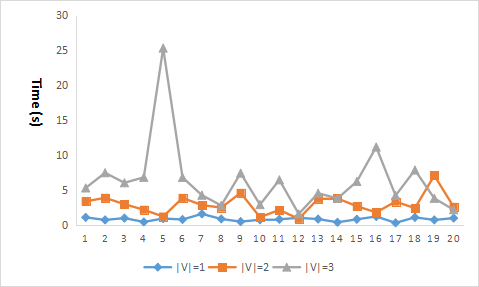
\includegraphics[width=7cm]{time_4_12.png}
	% 		\caption{Time used to compute forgetting for length 12}
	% 		\label{fig:time_4_12}
	% 	\end{minipage}
	% 	\begin{minipage}[t]{0.48\textwidth}
	% 		\centering
	% 		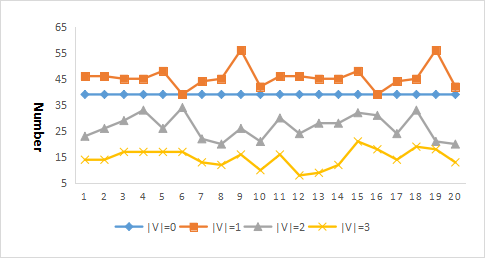
\includegraphics[width=7cm]{number-4-12.png}
	% 		\caption{The number of $\CTLsnf$ after the   Removing$\_$atoms process for length 12}
	% 		\label{fig:number_4_12}
	% 	\end{minipage}
	% \end{figure*}
	
	\begin{figure*}[!htb]
		\centering
		\subfigure[Time used to compute forgetting]{
			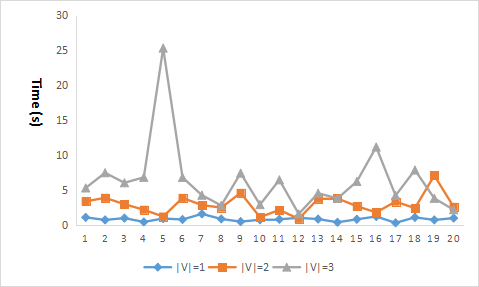
\includegraphics[width=7cm]{time_4_12.png}
		}
		\subfigure[The number of $\CTLsnf$ clauses]{
			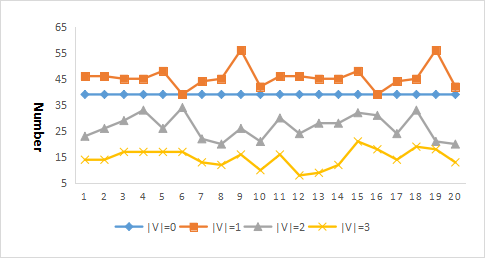
\includegraphics[width=7cm]{number-4-12.png}
		}
		\caption{The results of the cases for $\varphi_i=12$.}
		\label{fig:for12}
	\end{figure*}
	For the length $12$ of $\varphi_i$, the CPU time cost (in seconds) and the remaining number of $\CTLsnf$ clauses after the Removing\_atoms process of computing $\emph{ERes}(\varphi, V)$ are reported in (a) and (b) of Figure~\ref{fig:for12}, respectively, where $|V|$ ranges from 1 to 3. Figure~\ref{fig:for16} illustrates the same analysis for the length $16$.
	%For the length $16$ of $\varphi_i$, the CPU time cost (in seconds) and the number of $\CTLsnf$ clauses of computing $\emph{ERes}(\varphi, V)$ are reported in (a) and (b) of Figure~\ref{fig:for16}, respectively, where $|V|$ also ranges from 1 to 3.
	
	% \begin{figure*}[htbp]
	% 	\centering
	% 	\begin{minipage}[t]{0.48\textwidth}
	% 		\centering
	% 		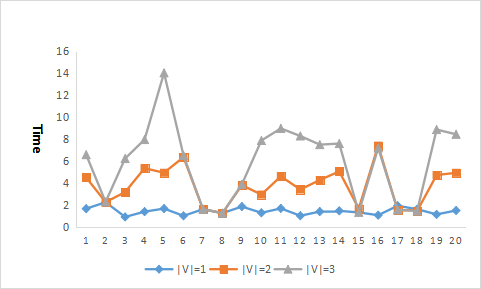
\includegraphics[width=7cm]{time_4_16.png}
	% 		\caption{Time used to compute forgetting for length 16}
	% 		\label{fig:time_4_16}
	% 	\end{minipage}
	% 	\begin{minipage}[t]{0.48\textwidth}
	% 		\centering
	% 		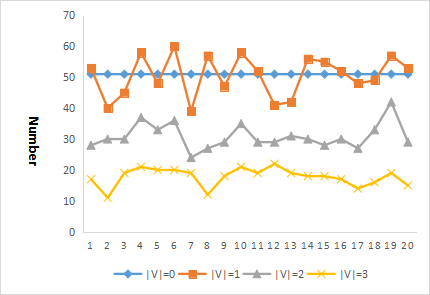
\includegraphics[width=7cm]{number-4-16.png}
	% 		\caption{The number of $\CTLsnf$ after the  Removing$\_$atoms process for length 16}
	% 		\label{fig:number_4_16}
	% 	\end{minipage}
	% \end{figure*}
	
	\begin{figure*}[!htb]
		\centering
		\subfigure[Time used to compute forgetting]{
			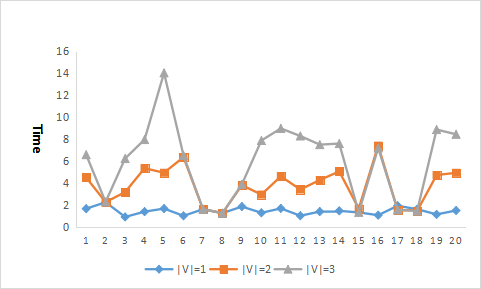
\includegraphics[width=7cm]{time_4_16.png}
		}
		\subfigure[The number of $\CTLsnf$ clauses]{
			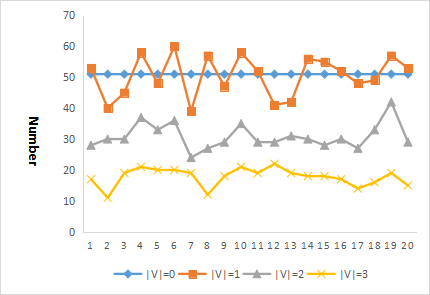
\includegraphics[width=7cm]{number-4-16.png}
		}
		\caption{The results of the cases for $\varphi_i=16$.}
		\label{fig:for16}
	\end{figure*}
	
	Observe that in all these figures, our Prolog program computes $\CTLforget(\varphi,V)$ in a few seconds for $|V|\in\{1,2,3\}$. Moreover, as we forget more atoms from $\varphi$, the number of $\CTLsnf$ clauses obtained after the Removing\_atoms process will also be decreasing.
	
	%\subsection{The Model-based Method}
	
	\subsection{Computing SNC by Forgetting}
	%In this subsection, we show the
	This section presents the empirical evaluation regarding \emph{time performance} and \emph{computing performance} of computing the SNC using forgetting.
	The time performance refers to how much time  it takes to calculate SNC, while the computing performance refers to the percentage of the formulas that an SNC exists for, in a given set of formulas defined on  a set $\Ha$ of atoms where $|\Ha|=50$.
	%For convenience, we define the length of a 3-\CNF\ formula as the number of clauses.
	
	Let $\varphi$ be a 3-\CNF\ formula, $V$ be a set of atoms, and $q$ be an atom with $q\in \Var(\varphi)-V$.
	It follows from Theorem~\ref{thm:SNC:WSC:forget} that if the result of forgetting the atoms in $\Var(\varphi \wedge q) - V$ from $\varphi \wedge q$ exists, then the SNC of $q$ on $V$ under $\varphi$ always exists.
	Accordingly, the SNC always exists in PL. %The time performance is shown in Figure~\ref{ProCNFtime}.
	Figure~\ref{fig:ProTime}(a)  shows the time performance.
	
	
	
	% \begin{figure*}[htbp]
	% 	\centering
	% 	\begin{minipage}[t]{0.48\textwidth}
	% 		\centering
	% 		\includegraphics[width=7cm]{ProAveTime.png}
	% 		\caption{Time performance of computing SNC in CPL}
	% 		\label{ProCNFtime}
	% 	\end{minipage}
	% 	\begin{minipage}[t]{0.48\textwidth}
	% 		\centering
	% 		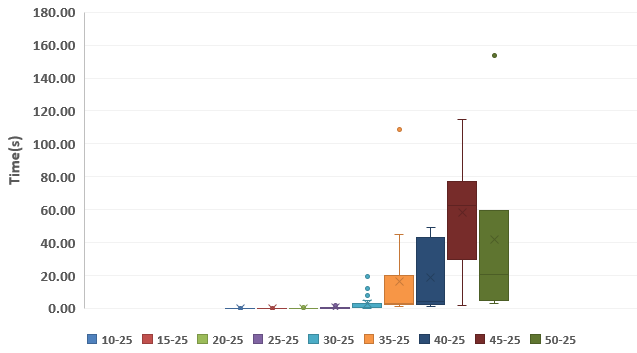
\includegraphics[width=7cm]{ProBox(10-50)_25.png}
	% 		\caption{The Boxplots of $|V|=25$ and $|\varphi| \in \{10, 15,\dots, 50\}$.}
	% 		\label{ProBox(10-50)_25}
	% 	\end{minipage}
	% \end{figure*}
	
	\begin{figure*}[!htb]
		\centering
		\subfigure[Time performance]{
			\includegraphics[width=7cm]{ProAveTime.png}
		}
		\subfigure[The Boxplots of $|V|=25$ and $|\varphi|~\in~ \{10, 15,\dots, 50\}$]{
			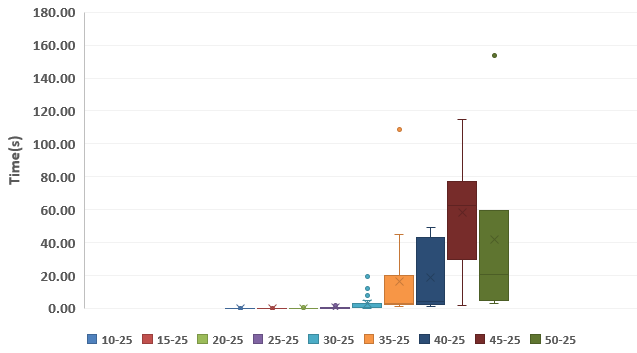
\includegraphics[width=7cm]{ProBox(10-50)_25.png}
		}
		\caption{The time performance of computing SNC in PL.}
		\label{fig:ProTime}
	\end{figure*}
	
	
	In Figure~\ref{fig:ProTime}(a), the numbers of atoms in $V$ and clauses in $\varphi$ are reported in Y-axis and X-axis, respectively: $|V| \in \{5, 10, 15, \dots, 40, 45\}$ and $|\varphi| \in \{10, 15, \dots, 45, 50\}$.
	Z-axis indicates the average time used to calculate 20 formulas.
	We see that the formulas with shorter lengths take less time.
	Moreover, the longer  $|V|$ gets, i.e., the fewer atoms you have to forget, hence the lesser time it requires.
	% Besides, the boxplots in (b) of Figure~\ref{fig:ProTime} show that as the length of the formula gets longer, it takes more time.
	The time spent to compute the SNC in the case of $|\varphi| \in \{10, \dots, 25\}$ are around its median, while there are some singularities when $|\varphi| \in \{30, 35, 50\}$ (See Figure 6(b)).
	
	Figure~\ref{fig:CtlTime} shows the time performance (a) and the computing perormance (b) for a \CTL\ formula $\varphi$ of the form $\varphi_1\wedge \ALL \NEXT \varphi_2  \wedge \EXIST \NEXT \varphi_3$
	where $\varphi_i~(i=1,2,3)$ are randomly generated 3-\CNF\ clauses in PL, and X-axis corresponds to $|\varphi_i|\in \{5, 6, 7, \dots, 14\}$, whereas Y-axis corresponds to  $|V| \in \{15, 16, \dots, 23, 24\}$.
	It is worth noting that 40 formulas have been calculated for every situation here, i.e., Z-axis indicates the average time used to calculate it.
	%This subsection shows which formulas do and do not have SNC, i.e., the SNC of $q$ on $V$ under $\varphi$.
	
	In Figure~\ref{fig:CtlTime}(a), we observe the same behaviour and the intuition as in   Figure~\ref{fig:ProTime}(a).
	Figure~\ref{fig:CtlTime}(b), however, shows that the SNC  exists for most formulas, especially, about 80\% when $|\varphi_i|=5$ and $|V|=16$.
	Furthermore, the boxplots in Figure~\ref{CtlBox14_(14-24)} indicate that given a formula, the more atoms that is needed to be forgotten, the more time it takes.
	%Extremely, the case of `14-45' was not calculated within the time (i.e. 1080s) and memory we specified.
	
	
	% \begin{figure*}[htbp]
	% 	\centering
	% 	\begin{minipage}[t]{0.48\textwidth}
	% 		\centering
	% 		\includegraphics[width=7cm]{CtlAveTime(1).png}
	% 		\caption{Time performance of computing SNC in \CTL}
	% 		\label{CtlCNFtime}
	% 	\end{minipage}
	% 	\begin{minipage}[t]{0.48\textwidth}
	% 		\centering
	% 		\includegraphics[width=7cm]{CtlNumPercent.png}
	% 		\caption{The Boxplots of $|\Var(\varphi)|=14$ and $|V| \in \{14, 15,\dots, 24\}$.}
	% 		\label{CtlCNFnum}
	% 	\end{minipage}
	% \end{figure*}
	
	\begin{figure*}[!htb]
		\centering
		\subfigure[Time performance]{
			\includegraphics[width=7cm]{CtlAveTime(1).png}
		}
		\subfigure[Computing performance]{
			\includegraphics[width=7cm]{CtlNumPercent.png}
		}
		\caption{The performances of computing SNC in \CTL.}
		\label{fig:CtlTime}
	\end{figure*}
	
	
	\begin{figure*}[ht]
		\centering
		\includegraphics[width=7cm]{CtlBox14_(14-24).png}\\
		\caption{Time Boxplots of computing SNC in \CTL}\label{CtlBox14_(14-24)}
	\end{figure*}
	
	Overall, our algorithm can compute the SNC (WSC) in most of the  cases and is efficient when the number of atoms that is to be forgotten is small, or the length of the formula is short.
	Moreover, the number of  $\CTLsnf$ clauses decreases as we forget more atoms.
	%when it does not need to consider some atoms of the given property.
	%the number of $\CTLsnf$ clauses obtained after the process will be diminishing
	
	%And the relation between SNC and WSC is shown in Table~dd (可能这不是很好算,因为得先计算出一个必要条件,还要计算出一个WSC).
	%\begin{example}
	%	Let $\varphi=((y_1 \vee y_2 \vee y_4) \wedge (\neg y_1 \vee y_2 \vee y_3) \wedge (y_1 \vee y_2 \vee y_3) \wedge (y_1 \vee y_2 \vee \neg y_4)) \wedge \ALL\NEXT((\neg y_1 \vee y_3 \vee y_4) \wedge (\neg y_1 \vee \neg y_2 \vee y_4) \wedge (\neg y_1 \vee y_2 \vee \neg y_3) \wedge (\neg y_2 \vee \neg y_3 \vee \neg y_4) \wedge (y_2 \vee y_3 \vee \neg y_4)) \wedge \EXIST\NEXT((\neg y_1 \vee \neg y_2 \vee y_4) \wedge (\neg y_1 \vee y_2 \vee \neg y_3) \wedge (\neg y_1 \vee y_2 \vee y_3) \wedge (y_2 \vee \neg y_3 \vee \neg y_4) \wedge (y_1 \vee \neg y_3 \vee \neg y_4)) \wedge q$ be a \CTL\ formula with four atoms, $V = \{y_1,y_4\}$ be a set of atoms appearing in $\varphi$, and $q$ be an atom in $\Var(\varphi) - V$. Then the SNC of $q$ on $V$ under $\varphi$ exists by using our Algorithm~\ref{alg:compute:forgetting:by:Resolution}. During calculation, the result after the eliminating index process is as follows:
	%	$\begin{array}{lll}
	%		z \rto \EXIST\NEXT(x_1 \wedge (y_4 \vee \neg x_2 \vee \neg y_1) \wedge (y_4 \vee \neg y_1)) &
	%		z \rto \ALL\NEXT x_2 &
	%		z \rto \ALL\NEXT (y_4 \vee \neg y_1) \\
	%		\start \rto (y_4 \vee \neg x_2 \vee \neg y_1) &
	%		\top \rto (y_4 \vee \neg x_1 \vee \neg y_1)&
	%		\start \rto z 	\\
	%		\top \rto (y_4 \vee \neg x_2 \vee \neg y_1 \vee \neg z) & \top \rto (y_4 \vee \neg x_2 \vee \neg y_1)
	%	\end{array}
	%	$
	%	
	%	Moreover, the result of using Ackermann's Lemma is as follows:\\
	%	$\begin{array}{ll}
	%	z &\rto (((y_4 \vee \neg x_2 \vee \neg y_1) \wedge (\ALL \NEXT (y_4\vee \neg y_1))) \wedge (\ALL \NEXT x_2))\wedge (\EXIST \NEXT (x_1 \wedge (y_4\vee \neg y_1)))\\
	%	 x_1 & \rto (y_4 \vee \neg y_1)\\
	%	x_2 & \rto (y_4\vee \neg y_1))	
	%	\end{array}	
	%    $
	%
	%    In this case, it is easy to obatin the SNC of $q$ on $V$ under $\varphi$.
	%\end{example}
	
	%It is easy to see from Theorem~\ref{thm:SNC:WSC:forget} that if the result of forgetting the atoms in $\Var(\varphi \wedge q) - V$ from $\varphi \wedge q$ exists then the SNC of $q$ on $V$ under $\varphi$ always exists. Therefore, the following tables show the statistical results of whether SNC exists or not.
	
	%Moreover, Table~dd shows that if we know the SNC before then it is easy to compute the WSC (可能这不是很好算,因为得先计算出一个必要条件,还要计算出一个WSC).
	
	%\subsection{Updating Knowledge by Forgetting}
	\section{Concluding Remarks}
	\subsection{Summary}
	In this paper, we presented the notion of forgetting for \CTL\
	which enables computing WSC (SNC) of specifications and knowledge update.
	To achieve this, we introduced  the notions of $V$-bisimulation and $\tuple{V,I}$-bisimulation, which can be considered  a simple variable-based generalization of classical bisimulation.
	Furthermore, we studied formal properties (i.e., homogeneity, modularity, and commutativity) of forgetting and a resolution-based method to compute forgetting.
	In particular, we  have shown that the notion of forgetting in bounded \CTL\ satisfies the existing postulates of forgetting.
	Moreover, we proposed a model-based algorithm to compute the forgetting of a given formula and a set of variables in bounded \CTL.
	We coupled our approach with a syntactic one and introduced a resolution-based algorithm which has been implemented in Prolog.  Our experimental results show that it is relatively efficient to compute forgetting and can be used to compute the SNC in most cases.
	%Experiments has been
	
	
	
	
	
	\subsection{Discussion and Future Avenues of Research}
	
	Our  study explores how to abstract the information, which is critical to designing a system, from a specification inthe context of a \CTL\ formula. In doing so, we have given a forgetting-based method from both syntax (resolution-based) and semantical (model-based) points. Based on this, we demonstrated how can forgetting be used to computed WSC (SNC) and knowledge update.
	
	We have shown that our forgetting is not close in \CTL. This analysis supports the theory that the \CTL\ is a failure of uniform interpolation. Nevertheless, we show that there is a special fragment of \CTL\ in which the forgetting is close. It is not trivial to find more fragments in the future since we believe most properties of a system can be expressed by those \CTL\ fragments. And in this case, distilling some information from it by forgetting is easy. Moreover, the results indicate that forgetting is close in bounded \CTL, which is the fact that the result of forgetting some atoms from a \CTL\ formula can always be expressed by a \CTL\ formula.
	
	There remain some interesting directions which deserve further investigation: First, although the initial results for the  complexity analysis of some problems (including model checking and  Entailment of forgetting) for the $\CTL_{\ALL\FUTURE}$ fragment was reported in our earlier work  KR~\cite{renyansfirstpaper}, a thorough investigation is still needed for the general case (namely, \CTL). Second, we did not yet resolve whether the resolution-based method is complete for forgetting. Third, we still do not explore how can the WSC obtained by our algorithm be used to update the original model system.
	More specifically, when a transition system $\cal M$ does not satisfy a specification $\phi$, one can evaluate the weakest sufficient condition  $\psi$ over a signature $V$ under which ${\cal M}$ satisfies $\phi$, viz., ${\cal M}\models\psi\rto \phi$ and $\psi$ mentions only atoms from $V$. It is worthwhile to explore how the condition $\psi$ can guide the design of a new transition system ${\cal M}'$ satisfying $\phi$.
	Last but not least, different fragments, in which the result of forgetting always exists, is of central interest for the future research avenue.
	% \section{Experimental Results}
	
	% \label{results}
	
	%  [section ommitted]
	
	% \section{A Theoretical Model}
	% \label{analysis}
	
	%  [section ommitted]
	
	% \section{Discussion}
	
	%  [section ommitted]
	
	%\acks{The authors wish to thank .
	%}
	
	
	\vskip 0.2in
	\bibliography{sample}
	\bibliographystyle{theapa}
	
	
	\clearpage
	\appendix
	\renewcommand{\appendixname}{Appendix~\Alph{section}}
	%\section{Supplementary Material: Proof Appendix}
	
	
	\section{Notations for the proofs}
	
	For convenience, we give the following notations:
	\begin{itemize}
		\item[(1)] By $T \wedge \varphi$, we mean $\bigwedge_{\psi\in T} \psi \wedge \varphi$, where $T$ is a finite set of formulas.
		\item[(2)] Let $C$ and $C'$ be two formulas, we say $C$ and $C'$ are \emph{resolvable} if there is a resolution rule using $C$ and $C'$ as the premises on some given atom.
		\item[(3)] For any two $\Ind$-structures $\Hm_i=(S_i, R_i, L_i, [\_]_i, s_0^i)$ with $i\in \{1, 2\}$, if $(\Hm_1, s_0^1) \lrto_{\tuple{V,I}} (\Hm_2, s_0^2)$, then we have $(\Hm_1', s_0^1) \lrto_V (\Hm_2', s_0^2)$ under \CTL, where $\Hm_i'=(S_i, R_i, L_i, s_0^i)$ with $i\in \{1, 2\}$.
		%Besides, we assume each atom in $V'$ (the set of atoms introduced in the transition progress) is false in all the states of any $\Ind$-model of a given formula.
		\item[(4)]
		%     Moreover, two paths $\pi_i=(s_{i,1},s_{i,2},\ldots)$ of $\Hm_i$ with $i\in \{1,2\}$
		% are $V$-{\em bisimilar} if
		% ${\cal K}_{1,j} \lrto_V {\cal K}_{2,j}$ for every $j\ge 1$
		% where ${\cal K}_{i,j}=(\Hm_i,s_{i,j})$.
		And when the $\Hm_i$ $(i=1,2)$ is clear from the context, we also use $(s_1, s_2)\in \Hb_n$ to replace $((\Hm_1,s_1),(\Hm_2,s_2))\in \Hb_n$.
	\end{itemize}
	
	
	
	
	
	\section{Proofs for Section~\ref{forgetting_ctl}}
	% \noindent \textbf{Section}~\ref{forgetting_ctl} \textbf{Semantic Forgetting in \CTL}
	
	\noindent\textbf{Proposition}~\ref{pro:VI:prop:bisimilar:V}
	Let $V_1,V_2\subseteq\cal A$, $I_1, I_2 \subseteq \Ind$
	and ${\cal K}_i=({\cal M}_i,s_i)$ with $i\in \{1,2,3\}$ be $\Ind$-structures
	s.t.
	${\cal K}_1\lrto_{\tuple{V_1, I_1}}{\cal K}_2$ and ${\cal K}_2\lrto_{\tuple{V_2,I_2}}{\cal K}_3$.
	Then:
	\begin{enumerate}[(i)]
		\item ${\cal K}_1\lrto_{\tuple{V_1\cup V_2, I_1 \cup I_2}}{\cal K}_3$;
		\item If $V_1 \subseteq V_2$ and $I_1 \subseteq I_2$ then ${\cal K}_1 \lrto_{\tuple{V_2, I_2}} {\cal K}_2$.
	\end{enumerate}
	\begin{proof}
		%This can be proved similarly with Proposition~\ref{prop:bisimilar:V}.
		(i) Let ${\cal M}_j=(S_i,R_i,L_i,[\_]_i,s_0^i)~(i=1,2,3)$, $s_1 \lrto_\tuple{V_1, I_1} s_2$ via a binary relation $\Hb$, and $s_2 \lrto_\tuple{V_2, I_2} s_3$ via a binary relation $\Hb''$. Let $\Hb' = \{(w_1, w_3)\mid (w_1, w_2)\in \Hb$ and $(w_2, w_3)\in \Hb''\}$. To prove ${\cal K}_1\lrto_{V_1\cup V_2}{\cal K}_3$, we will prove that $\Hb'$ is a  $\tuple{V_1 \cup V_2, I_1\cup I_2}$-bisimulation containing $(s_1, s_3)$. It's evident that $(s_1, s_3) \in \Hb'$ due to $(s_1,s_2)\in \Hb$ and $(s_2, s_3)\in \Hb''$.
		
% 		Let ${\cal M}_j=(S_i,R_i,L_i,[\_]_i,s_0^i)~(i=1,2,3)$, $s_0^1 \lrto_\tuple{V_1, I_1} s_0^2$ via a binary relation $\Hb$, and $s_0^2 \lrto_\tuple{V_2, I_2} s_0^3$ via a binary relation $\Hb''$. Let $\Hb' = \{(w_1, w_3)\mid (w_1, w_2)\in \Hb$ and $(w_2, w_3)\in \Hb''\}$. To prove ${\cal K}_1\lrto_{V_1\cup V_2}{\cal K}_3$, we will prove that $\Hb'$ is a  $\tuple{V_1 \cup V_2, I_1\cup I_2}$-bisimulation containing $(s_0^1, s_0^3)$. It's evident that $(s_0^1, s_0^3) \in \Hb'$ due to $(s_0^1,s_0^2)\in \Hb$ and $(s_0^2, s_0^3)\in \Hb''$.
		% 		from the (a), (b) and (c) of the previous step (iii) of $X$-bisimulation (where $X$ is a set of atoms).
		For all $(w_1, w_3) \in \Hb'$ and $j \not \in (I_1 \cup I_2)$:
		\begin{enumerate}[(a)]
			\item there exists $w_2 \in S_2$ s.t.  $(w_1,w_2)\in \Hb$ and $(w_2, w_3)\in \Hb''$, and for all $q \notin V_1$, $q \in L_1(w_1)$ iff $q \in L_2(w_2)$ by $w_1 \lrto_{V_1} w_2$ and for all $q' \notin V_2$, $q'\in L_2(w_2)$ iff $q'\in L_3(w_3)$ by $w_2 \lrto_{V_2} w_3$. Then we have for all $r\notin V_1 \cup V_2$, $r \in L_1(w_1)$ iff $r \in L_3(w_3)$.
			
			\item $\forall u_1\in S_1$, if $(w_1, u_1) \in R_1$, then $\exists u_2\in S_2$ s.t.  $(w_2, u_2) \in R_2$ and $(u_1,u_2)\in \Hb$ (due to $(w_1,w_2)\in \Hb$ and $(w_2, w_3) \in \Hb''$ by the definition of $\Hb'$); and then $\exists u_3 \in S_3$ s.t.  $(w_3, u_3) \in R_3$ and $(u_2, u_3) \in \Hb''$, hence $(u_1, u_3) \in \Hb'$ by the definition of $\Hb'$.
			
			\item $\forall u_3\in S_3$, if $(w_3, u_3) \in R_3$, then $\exists u_2\in S_2$ s.t.  $(w_2, u_2) \in R_2$ and $(u_2, u_3) \in \Hb_2$; and then $\exists u_1 \in S_1$ s.t.  $(w_1, u_1) \in R_1$ and $(u_1, u_2) \in \Hb$, hence $(u_1, u_3) \in \Hb'$ by the definition of $\Hb'$.
			
			\item $\forall (w_1, r_1) \in [j]_1$, $\exists (w_2, r_2) \in [j]_2$ s.t. $(w_1, w_2)\in \Hb$ and $(r_1, r_2) \in \Hb$; and then $\exists (w_3, r_3)\in [j]_3$ s.t. $(w_2, w_3)\in \Hb''$ and $(r_2, r_3) \in \Hb''$. Therefore, $(w_1, w_3) \in \Hb''$ and $(r_1, r_3) \in \Hb''$.
			
			\item similar to $(d)$, we can show that $\forall (w_3, r_3)\in [j]_3$, $\exists(w_1, r_1)\in [j]_1$ s.t. $(w_1, w_3) \in \Hb''$ and $(r_1, r_3) \in \Hb''$.
		\end{enumerate}
		
		(ii) Supposing $\Hb_\tuple{V_1, I_1}$ is a $\tuple{V_1,I_1}$-bisimulation between $\Hm_1$ and $\Hm_2$ s.t. $(s_1, s_2)\in \Hb_\tuple{V_1, I_1}$. We will show that $\Hb_\tuple{V_1, I_1}$ is also a $\tuple{V_2, I_2}$-bisimulation between $\Hm_1$ and $\Hm_2$ s.t. $(s_1, s_2)\in \Hb_\tuple{V_1, I_1}$.
		For all $(w_1, w_2) \in \Hb_\tuple{V_1, I_1}$ and $j\not \in I_2$, there is:
		\begin{itemize}
			\item $L_1(w_1) - V_2 = L_2(w_2) -V_2$ since $L_1(w_1) - V_1 = L_2(w_2) -V_1$ and $V_1 \subseteq V_2$;
			\item $\forall r_1 \in S_1$, if $(w_1,r_1) \in R_1$ then $\exists r_2\in S_2$ s.t. $(w_2,r_2)\in R_2$ and $(r_1,r_2) \in \Hb_\tuple{V_1, I_1}$ since $\Hb_\tuple{V_1, I_1}$ is a $\tuple{V_1, I_1}$-bisimulation between $\Hm_1$ and $\Hm_2$; and
			\item $\forall r_2 \in S_2$, if $(w_2,r_2) \in R_2$ then $\exists r_1\in S_1$ s.t. $(w_1,r_1)\in R_1$ and $(r_1,r_2) \in \Hb_\tuple{V_1, I_1}$ since $\Hb_\tuple{V_1, I_1}$ is a $\tuple{V_1, I_1}$-bisimulation between $\Hm_1$ and $\Hm_2$;
			\item $\forall (w_1, r_1) \in [j]_1$, $\exists (w_2, r_2) \in [j]_2$ s.t. $(w_1, w_2)\in \Hb_\tuple{V_1, I_1}$ and $(r_1, r_2) \in \Hb_\tuple{V_1, I_1}$ since $\Hb_\tuple{V_1, I_1}$ is a $\tuple{V_1, I_1}$-bisimulation between $\Hm_1$ and $\Hm_2$;  and
			
			\item $\forall (w_2, r_2)\in [j]_2$, $\exists(w_1, r_1)\in [j]_1$ s.t. $(w_1, w_2) \in \Hb_\tuple{V_1, I_1}$ and $(r_1, r_2) \in \Hb_\tuple{V_1, I_1}$ since $\Hb_\tuple{V_1, I_1}$ is a $\tuple{V_1, I_1}$-bisimulation between $\Hm_1$ and $\Hm_2$.
		\end{itemize}
	\end{proof}
	
	\noindent\textbf{Proposition}~\ref{prop:bisimilar:V} 	Let $i\in \{1,2\}$, $V_1,V_2\subseteq\cal A$, $s_i'$s be two states,
	$\pi_i'$s be two paths
	and ${\cal K}_j=({\cal M}_j,s_j)~(j=1,2,3)$ be$\Ind$-structures
	s.t.
	${\cal K}_1\lrto_{V_1}{\cal K}_2$ and ${\cal K}_2\lrto_{V_2}{\cal K}_3$.
	Then:
	\begin{enumerate}[(i)]
		\item ${\cal K}_1\lrto_{V_1\cup V_2}{\cal K}_3$;
		\item If $V_1 \subseteq V_2$ then ${\cal K}_1 \lrto_{V_2} {\cal K}_2$;
		\item $s_1'\lrto_{V_i}s_2'~(i=1,2)$ implies $s_1'\lrto_{V_1\cup V_2}s_2'$;
		\item $\pi_1'\lrto_{V_i}\pi_2'~(i=1,2)$ implies $\pi_1'\lrto_{V_1\cup V_2}\pi_2'$;
		\item for each path $\pi_{s_1}$ of $\Hm_1$ there is a path $\pi_{s_2}$  of $\Hm_2$ s.t. $\pi_{s_1} \lrto_{V_1} \pi_{s_2}$, and vice versa.
	\end{enumerate}
	
	\begin{proof}
		%We prove the cases of $\MPK$-structures, and the cases of $\Ind$-structures are trivial.
		(i) Let ${\cal M}_j=(S_j,R_j,L_j,[\_]_j,s_0^j)~(j=1,2,3)$, $s_1 \lrto_{V_1} s_2$ via a binary relation $\Hb$, and $s_2 \lrto_{V_2} s_3$ via a binary relation $\Hb''$. Let $\Hb' = \{(w_1, w_3)\mid (w_1, w_2)\in \Hb$ and $(w_2, w_3)\in \Hb''\}$. To prove ${\cal K}_1\lrto_{V_1\cup V_2}{\cal K}_3$, we will prove that $\Hb'$ is a  $V_1 \cup V_2$-bisimulation containing $(s_1, s_3)$. It's evident that $(s_1, s_3) \in \Hb'$ due to $(s_1,s_2)\in \Hb$ and $(s_2, s_3)\in \Hb''$.
		% 		from the (a), (b) and (c) of the previous step (iii) of $X$-bisimulation (where $X$ is a set of atoms).
		For all $(w_1, w_3) \in \Hb'$:
		\begin{enumerate}[(a)]
			\item there exists $w_2 \in S_2$ s.t.  $(w_1,w_2)\in \Hb$ and $(w_2, w_3)\in \Hb''$, and for all $q \notin V_1$, $q \in L_1(w_1)$ iff $q \in L_2(w_2)$ by $w_1 \lrto_{V_1} w_2$ and for all $q' \notin V_2$, $q'\in L_2(w_2)$ iff $q'\in L_3(w_3)$ by $w_2 \lrto_{V_2} w_3$. Then we have for all $r\notin V_1 \cup V_2$, $r \in L_1(w_1)$ iff $r \in L_3(w_3)$.
			\item $\forall u_1\in S_1$, if $(w_1, u_1) \in R_1$, then $\exists u_2\in S_2$ s.t.  $(w_2, u_2) \in R_2$ and $(u_1,u_2)\in \Hb$ (due to $(w_1,w_2)\in \Hb$ and $(w_2, w_3) \in \Hb''$ by the definition of $\Hb'$); and then $\exists u_3 \in S_3$ s.t.  $(w_3, u_3) \in R_3$ and $(u_2, u_3) \in \Hb''$, hence $(u_1, u_3) \in \Hb'$ by the definition of $\Hb'$.
			\item $\forall u_3\in S_3$, if $(w_3, u_3) \in R_3$, then $\exists u_2\in S_2$ s.t.  $(w_2, u_2) \in R_2$ and $(u_2, u_3) \in \Hb_2$; and then $\exists u_1 \in S_1$ s.t.  $(w_1, u_1) \in R_1$ and $(u_1, u_2) \in \Hb$, hence $(u_1, u_3) \in \Hb'$ by the definition of $\Hb'$.
		\end{enumerate}
		
		(ii) Supposing $\Hb_{V_1}$ is a $V_1$-bisimulation between $\Hm_1$ and $\Hm_2$ s.t. $(s_1, s_2)\in \Hb_{V_1}$. We will show that $\Hb_{V_1}$ is also a $V_2$-bisimulation between $\Hm_1$ and $\Hm_2$ s.t. $(s_1, s_2)\in \Hb_{V_1}$.
		For all $(w_1, w_2) \in \Hb_{V_1}$, there is:
		\begin{itemize}
			\item $L_1(w_1) - V_2 = L_2(w_2) -V_2$ since $L_1(w_1) - V_1 = L_2(w_2) -V_1$ and $V_1 \subseteq V_2$;
			\item $\forall r_1 \in S_1$, if $(w_1,r_1) \in R_1$ then $\exists r_2\in S_2$ s.t. $(w_2,r_2)\in R_2$ and $(r_1,r_2) \in \Hb_{V_1}$ since $\Hb_{V_1}$ is a $V_1$-bisimulation between $\Hm_1$ and $\Hm_2$; and
			\item $\forall r_2 \in S_2$, if $(w_2,r_2) \in R_2$ then $\exists r_1\in S_1$ s.t. $(w_1,r_1)\in R_1$ and $(r_1,r_2) \in \Hb_{V_1}$ since $\Hb_{V_1}$ is a $V_1$-bisimulation between $\Hm_1$ and $\Hm_2$.
		\end{itemize}
		
		(iii) is a special case of (ii) due to $V_i \subseteq (V_1 \cup V_2)$ with $i = 1, 2$. And then (iv) is evident from (iii).
		
		(v) This is obvious from the definition of $V$-bisimulation due to $s_1 \lrto_{V_1} s_2$ (i.e., ${\cal K}_1\lrto_{V_1}{\cal K}_2$).
		
	\end{proof}
	
	
	
	
	
	
	\noindent\textbf{Theorem}~\ref{thm:V-bisimulation:EQ}
	Let $V\subseteq\cal A$, ${\cal K}_i~(i=1,2)$ be two$\Ind$-structures s.t.
	${\cal K}_1\lrto_V{\cal K}_2$ and $\phi$ a formula with $\IR(\phi,V)$. Then
	${\cal K}_1\models\phi$ if and only if ${\cal K}_2\models\phi$.
	\\
	\begin{proof}
		This theorem can be proved by inducting on the formula $\phi$ and supposing $\Var(\phi) \cap V = \Empty$.
		Let ${\cal K}_1 = (\Hm, s)$ and ${\cal K}_2 = (\Hm', s')$.
		
		%Here we only prove the only-if direction. The other direction can be similarly proved.
		
		\textbf{Base case.} $\phi = p$ where $p \in \Ha - V$:\\
		$(\Hm, s) \models \phi$ iff $p\in L(s)$  \hfill  (by the definition of satisfiability) \\
		$\LRto$ $p \in L'(s')$ \hfill ($s \lrto_V s'$)\\
		$\LRto$ $(\Hm', s') \models \phi$
		
		\textbf{Step case.} (1) $\phi = \neg \psi$:\\
		$(\Hm, s) \models \phi$ iff $(\Hm, s) \not \models \psi$ \\
		$\LRto$ $(\Hm', s') \not \models \psi$  \hfill   (induction hypothesis)\\
		$\LRto$ $(\Hm', s') \models \phi$
		
		(2) $\phi = \psi_1 \vee \psi_2$:\\
		$(\Hm, s) \models \phi$\\
		$\LRto$ $(\Hm, s) \models \psi_1$ or $(\Hm, s) \models \psi_2$\\
		$\LRto$ $(\Hm', s') \models \psi_1$ or $(\Hm', s') \models \psi_2$   \hfill  (induction hypothesis)\\
		$\LRto$ $(\Hm', s') \models \phi$
		
		(3) $\phi = \EXIST \NEXT \psi$:\\
		%By Lemma~\ref{V_path}, we assume there are two paths $\pi = s, s_1, ...$ and $\pi' = s', s_1', ...$ such that $\pi \lrto_V \pi'$.\\
		$(\Hm, s) \models \phi$ \\
		$\LRto$ There is a path $\pi = (s, s_1, ...)$ s.t.  $(\Hm, s_1) \models \psi$\\
		$\LRto$ There is a path $\pi' = (s', s_1', ...)$ s.t.  $\pi \lrto_V \pi'$ \hfill   ($s \lrto_V s'$, Proposition~\ref{prop:bisimilar:V}(v))\\
		$\LRto$ $s_1 \lrto_V s_1'$  \hfill ($\pi \lrto_V \pi'$)\\
		$\LRto$ $(\Hm', s_1') \models \psi$  \hfill  (induction hypothesis)\\
		$\LRto$ $(\Hm', s') \models \phi$
		
		(4) $\phi = \EXIST \GLOBAL \psi$:\\
		$(\Hm, s) \models \phi$ \\
		$\LRto$ There is a path $\pi =(s=s_0, s_1, ...)$ s.t.  for each $i \geq 0$ there is $(\Hm, s_i) \models \psi$\\
		$\LRto$ There is a path $\pi' = (s'=s_0', s_1', ...)$ s.t.  $\pi \lrto_V \pi'$   \hfill ($s \lrto_V s'$, Proposition~\ref{prop:bisimilar:V}(v))\\
		$\LRto$ $s_i \lrto_V s_i'$ for each $i \geq 0$ \hfill ($\pi \lrto_V \pi'$)\\
		$\LRto$ $(\Hm', s_i') \models \psi$ for each $i \geq 0$  \hfill  (induction hypothesis)\\
		$\LRto$ $(\Hm', s') \models \phi$
		
		(5) $\phi = \EXIST (\psi_1 \UNTIL \psi_2)$:\\
		%\textbf{Case} $\varphi = \MPE \FUTURE \psi$:
		$(\Hm, s) \models \phi$ \\
		$\LRto$ There is a path $\pi= (s=s_0, s_1, ...)$ such that there is $i \geq 0$ such that $(\Hm, s_i) \models \psi_2$, and for all $0 \leq j < i$, $(\Hm, s_j) \models \psi_1$\\
		$\LRto$ There is a path $\pi' = (s=s_0', s_1', ...)$ such that $\pi \lrto_V \pi'$  \hfill  ($s \lrto_V s'$, Proposition~\ref{prop:bisimilar:V}(v))\\
		$\LRto$ $(\Hm', s_i') \models \psi_2$, and for all $0 \leq j < i$ $(\Hm', s_j') \models \psi_1$   \hfill   (induction hypothesis)\\
		$\LRto$ $(\Hm', s') \models \phi$
	\end{proof}
	
	
	
	
	
	
	\noindent\textbf{Theorem}~\ref{thm:PL:CTL}
	Let $\varphi$ be a PL formula and $V\subseteq \Ha$, then
	\[
	\CTLforget(\varphi, V) \equiv \Forget(\varphi, V).
	\]
	\\
	\begin{proof}
		Let $\Hm = (S, R, L,[\_], s)$ and $\Hm' = (S', R', L',[\_]', s')$.
		
		On the one hand, for each $(\Hm, s) \in \Mod(\CTLforget(\varphi, V))$, there exists a $(\Hm', s') \in \Mod(\varphi)$ s.t. $s\lrto_V s'$. Thus, $L(s)-V = L'(s')-V$. Hence, $(\Hm, s)$ is a model of $\Forget(\varphi, V)$.
		
		On the other hand, for each $(\Hm, s) \in \Mod(\Forget(\varphi, V))$, there exists a $(\Hm', s') \in \Mod(\varphi)$ s.t. $L(s)-V = L'(s')-V$. We can construct an initial$\Ind$-structure $(\Hm_1, s_1)$ s.t. $\Hm_1=(S_1, R_1, L_1,[\_]_1, s_1)$ with $S_1= (S - \{s\}) \cup \{s_1\}$, $R_1$ is the same as $R$, except replace $s$ with $s_1$, and $L_1$ is the same as $L$, except $L_1(s_1) = L'(s')$, where $L'$ is the label function of $M'$. It is clear that $(\Hm_1, s_1)$ is a model of $\varphi$ and $s_1 \lrto_V s$. Hence, $(\Hm, s)$ is a model of $\CTLforget(\varphi, V)$.
	\end{proof}
	
	
	
	
	\noindent \textbf{Lemma}~\ref{lem:KF:eq} Let $\varphi$ and $\alpha$ be two \CTL\ formulas and $q\not \in
	(\Var(\varphi) \cup \Var(\alpha))$. Then
	$\CTLforget(\varphi \wedge (q\lrto\alpha), q)\equiv \varphi$.\\
	\begin{proof}
		Let $\varphi' =\varphi \wedge (q\lrto\alpha)$. For any model $({\cal M},s)$ of $\CTLforget(\varphi', q)$ there is an initial$\Ind$-structure $({\cal M}',s')$ s.t.\ $({\cal M},s)\lrto_{\{q\}}({\cal M}',s')$ and $({\cal M}',s') \models \varphi'$. It's evident that $({\cal M}',s') \models \varphi$, and then $({\cal M},s) \models \varphi$ since $\IR(\varphi,\{q\})$ and $({\cal M},s)\lrto_{\{q\}}({\cal M}',s')$
		by Theorem~\ref{thm:V-bisimulation:EQ}.
		
		Let $(\Hm,s) \in \Mod(\varphi)$ with ${\cal M}=(S, R, L,[\_], s)$. We construct $(\Hm', s)$ with $\Hm' = (S, R, L',[\_], s)$ as follows:
		\begin{align*}
			& L':S \rto \Ha\ and\ \forall s^*\in S, L'(s^*) = L(s^*)-\{q\}\ \hbox{if}\ (\Hm, s^*) \not \models \alpha, else\ L'(s^*) = L(s^*)\cup\{q\}, \\
			& L'(s) = L(s) \cup\{q\}\ \hbox{if}\ (\Hm, s) \models \alpha,\ and\ L'(s) = L(s)-\{q\}\ otherwise.
		\end{align*}
		It is clear that $({\cal M}',s) \models \varphi$, $({\cal M}',s) \models q\lrto \alpha$ and
		$({\cal M}', s) \lrto_{\{q\}} ({\cal M}, s)$. Therefore $({\cal M}', s) \models \varphi \wedge (q\lrto\alpha)$, and then $({\cal M}, s) \models \CTLforget (\varphi \wedge (q\lrto\alpha), q)$ by
		$({\cal M}', s) \lrto_{\{q\}} ({\cal M}, s)$.
	\end{proof}
	
	
	
	
	
	\noindent\textbf{Proposition}~\ref{disTF} \textbf{(Modularity)}
	Given a formula $\varphi \in \CTL$, $V$ a set of atoms, and $p$ an atom s.t. $p \notin V$, then
	\[
	\CTLforget(\varphi, \{p\} \cup V) \equiv \CTLforget(\CTLforget(\varphi, p), V).
	\]\\
	\begin{proof}
		Let $(\Hm_1, s_1) $ with ${\cal M}_1=(S_1, R_1, L_1,s_1)$ be a model of $\CTLforget(\varphi, \{p\} \cup V)$. By the definition, there exists a model $(\Hm,s)$ with ${\cal M} = (S, R,L,[\_],s)$ of $\varphi$, such that $(\Hm_1, s_1)$ $\lrto_{\{p\} \cup V}$ $(\Hm, s)$. We construct an initial structure $(\Hm_2, s_2)$ with ${\cal M}_2 = (S_2, R_2, L_2,s_2)$ as follows:
		\begin{enumerate}[(1)]
			\item for $s_2$: let $s_2$ be the state such that:
			\begin{itemize}
				\item $p \in L_2(s_2)$ iff $p \in L_1(s_1)$,
				\item for all $q \in V$, $q \in L_2(s_2)$ iff $q\in L(s)$,
				\item for all other atoms $q'$, $q' \in L_2(s_2)$ iff $q' \in L_1(s_1)$ iff $q'\in L(s)$.
			\end{itemize}
			\item for another:
			\begin{enumerate}[(i)]
				\item for all pairs  $w \in S$ and $w_1 \in S_1$ s.t. $w \lrto_{\{p\} \cup V} w_1$, let $w_2 \in S_2$ and
				\begin{itemize}
					\item $p \in L_2(w_2)$ iff $p \in L_1(w_1)$,
					\item for all $q \in V$, $q \in L_2(w_2)$ iff $q\in L(w)$,
					\item for all other atoms $q'$, $q' \in L_2(w_2)$ iff $q' \in L_1(w_1)$ iff $q'\in L(w)$.
				\end{itemize}
				\item if $(w_1', w_1)\in R_1$, $w_2$ is constructed based on $w_1$ and $w_2'\in S_2$ is constructed based on $w_1'$, then $(w_2', w_2)\in R_2$.
				%And if $w' \Hr^i w$, $w_2$ is constructed based on $w$ and $w_2'\in \Hw_2$ is constructed based on $w'$, then $w_2' \Hr_2^i w_2$
				%\item if $\exists w_1'\in \Hw_1$ such that $w_1' \Hr_1 w_1$, then let $w_2' \in \Hw_2$, $w_2' \Hr_2 w_2$, and if $w_1' \neq s_1$ then do (i) for $w_2'$, else let$w_2' = s_2$.
			\end{enumerate}
			\item delete duplicated states in $S_2$ and pairs in $R_2$.
		\end{enumerate}
		Then we have $(\Hm, s) \lrto_{\{p\}} (\Hm_2, s_2)$ and $(\Hm_2, s_2) \lrto_V (\Hm_1, s_1)$. Thus, $(\Hm_2, s_2) \models \CTLforget(\varphi, p)$. Therefore $(\Hm_1, s_1) \models \CTLforget(\CTLforget(\varphi, p), V)$.
		
		On the other hand, suppose that $(\Hm_1, s_1)$ is a model of $\CTLforget(\CTLforget(\varphi, p), V)$, then there exists an initial structure $(\Hm_2, s_2)$ s.t. $(\Hm_2, s_2) \models \CTLforget(\varphi, p)$ and $(\Hm_2, s_2) \lrto_V (\Hm_1, s_1)$, and there exists $(\Hm, s)$ s.t. $(\Hm, s) \models \varphi$ and $(\Hm, s) \lrto_{\{p\}} (\Hm_2, s_2)$. Therefore, $(\Hm, s) \lrto_{\{p\} \cup V} (\Hm_1, s_1)$ by Proposition~\ref{prop:bisimilar:V}(i), and consequently, $(\Hm_1, s_1) \models \CTLforget(\varphi, \{p\} \cup V)$.
	\end{proof}
	
	
	
	
	\noindent\textbf{Proposition}~\ref{pro:ctl:forget:1}
	Let $\varphi$, $\varphi_i$, $\psi_i$ ($i=1,2$) be formulas in \CTL\ and $V\subseteq \Ha$. We have
	\begin{enumerate}[(i)]
		\item $\CTLforget(\varphi, V)$ is satisfiable iff $\varphi$ is;
		\item If $\varphi_1 \equiv \varphi_2$, then $\CTLforget(\varphi_1, V) \equiv \CTLforget(\varphi_2, V)$;
		\item If $\varphi_1 \models \varphi_2$, then $\CTLforget(\varphi_1, V) \models \CTLforget(\varphi_2, V)$;
		\item $\CTLforget(\psi_1 \vee \psi_2, V) \equiv \CTLforget(\psi_1, V) \vee \CTLforget(\psi_2, V)$;
		\item $\CTLforget(\psi_1 \wedge \psi_2, V) \models \CTLforget(\psi_1, V) \wedge \CTLforget(\psi_2, V)$;
		% \item If $\IR(\psi_1, V)$, then $\CTLforget(\varphi \wedge \psi_1, V) \equiv \CTLforget(\varphi, V) \wedge \psi_1$.
	\end{enumerate}
	
	\begin{proof}
		(i) ($\Rto$) Supposing $(\Hm, s)$ is a model of $\CTLforget(\varphi, V)$, then there is a model $(\Hm',s')$ of $\varphi$ s.t. $(\Hm,s) \lrto_V (\Hm',s')$ by the definition of $\CTLforget$.
		
		($\Lto$) Supposing $(\Hm, s)$ is a model of $\varphi$, then there is an initial structure $(\Hm',s')$ s.t. $(\Hm,s) \lrto_V (\Hm',s')$, and then $(\Hm',s') \models \CTLforget(\varphi, V)$ by the definition of $\CTLforget$.
		
		The (ii) and (iii) can be proved similarly.
		
		(iv) ($\Rto$) For all$(\Hm,s)\in \Mod(\CTLforget(\psi_1 \vee \psi_2, V))$, there exists $(\Hm',s')$ $\in$  $\Mod(\psi_1\vee \psi_2)$ s.t. $(\Hm,s) \lrto_V (\Hm',s')$ and $(\Hm',s') \models \psi_1$ or $(\Hm',s') \models \psi_2$ \\
		$\Rto$ there exists $(\Hm_1,s_1) \in \Mod(\CTLforget(\psi_1, V))$ s.t. $(\Hm',s') \lrto_V (\Hm_1,s_1)$ or there exists $(\Hm_2,s_2) \in \Mod(\CTLforget(\psi_2, V))$ s.t. $(\Hm',s') \lrto_V (\Hm_2,s_2)$ \\
		%$\Rto$ $(\Hm,s) \lrto_V (\Hm_1,s_1)$ or $(\Hm,s) \lrto_V (\Hm_2,s_2)$\\
		$\Rto$ $(\Hm,s) \models \CTLforget(\psi_1, V) \vee \CTLforget(\psi_2, V)$ by Theorem~\ref{thm:V-bisimulation:EQ}.
		
		($\Lto$) for all $(\Hm,s) \in \Mod(\CTLforget(\psi_1, V) \vee \CTLforget(\psi_2, V))$\\
		$\Rto$ $(\Hm,s) \models \CTLforget(\psi_1,V)$ or $(\Hm,s) \models \CTLforget(\psi_2,V)$\\
		$\Rto$ there is an initial structure $(\Hm_1,s_1)$ s.t. $(\Hm,s) \lrto_V (\Hm_1,s_1)$ and $(\Hm_1,s_1) \models \psi_1$ or  $(\Hm_1,s_1) \models \psi_2$\\
		$\Rto$ $(\Hm_1,s_1) \models \psi_1 \vee \psi_2$\\
		%$\Rto$ there is an initial structure $(\Hm_2,s_2)$ s.t. $(\Hm_1,s_1) \lrto_V (\Hm_2,s_2)$ and $(\Hm_2,s_2) \models \CTLforget(\psi_1 \vee \psi_2, V)$\\
		$\Rto$ $(\Hm,s) \models \CTLforget(\psi_1 \vee \psi_2, V)$ due to $(\Hm,s) \lrto_V (\Hm_1,s_1)$.
		
		The (v) can be proved as (iv).
	\end{proof}
	
	
	
	
	\textbf{Proposition}~\ref{pro:ctl:forget:2} \textbf{(Homogeneity)}
	Let $V\subseteq\cal A$ and $\phi \in \CTL$, then:% and $Q\in \{\EXIST, \ALL\}$.
	\begin{enumerate}[(i)]
		\item $\CTLforget(\ALL\NEXT\phi,V)\equiv \ALL\NEXT \CTLforget(\phi,V)$.
		\item $\CTLforget(\EXIST\NEXT\phi,V)\equiv\EXIST\NEXT \CTLforget(\phi,V)$.
		\item $\CTLforget(\ALL \FUTURE\phi,V)\equiv \ALL \FUTURE \CTLforget(\phi,V)$.
		\item $\CTLforget(\EXIST\FUTURE\phi,V)\equiv\EXIST\FUTURE \CTLforget(\phi,V)$.
	\end{enumerate}
	\begin{proof}
		Let $\Hm=(S, R, L,s_0)$ with the initial state $s_0$ and $\Hm'=(S', R', L',s_0')$ with the initial state $s_0'$, then we call $(\Hm', s_0')$ be a sub-structure of $(\Hm,s_0)$ if:
		\begin{itemize}
			\item $S' \subseteq S$ and $S'=\{s' \mid s'$ is reachable from $s_0'\}$,
			\item $R' =\{(s_1, s_2)\mid s_1, s_2 \in S'$ and $(s_1, s_2) \in R\}$,
			\item $L': S' \rto 2^\Ha$ and for all $s_1 \in S'$ there is $L'(s_1) = L(s_1)$, and
			\item $s_0'$ is $s_0$ or a state reachable from $s_0$.
		\end{itemize}
		
		(i) To prove $\CTLforget(\ALL \NEXT \phi, V) \equiv \ALL \NEXT(\CTLforget(\phi, V))$, the only thing we need to prove is \[\Mod(\CTLforget(\ALL \NEXT \phi, V)) = \Mod( \ALL\NEXT\CTLforget(\phi, V)).\]
		
		$(\Rto)$ For all $(\Hm', s') \in \Mod(\CTLforget(\ALL \NEXT \phi, V))$ there exists an initial structure $(\Hm, s)$ s.t. $(\Hm, s)\models \ALL \NEXT \phi$ and $(\Hm, s) \lrto_V (\Hm',s')$\\
		$\Rto$ for any sub-structure $(\Hm_1, s_1)$ of $(\Hm, s)$, there is $(\Hm_1, s_1) \models \phi$, where $s_1$ is a directed successor of $s$ \\
		$\Rto$ there is an initial structure $(\Hm_2, s_2)$ s.t. $(\Hm_2, s_2) \models \CTLforget(\phi,V)$ and $(\Hm_2, s_2) \lrto_V (\Hm_1,s_1)$\\
		$\Rto$ it is easy to construct an initial structure $(\Hm_3, s_3)$ by $(\Hm_2, s_2)$ s.t. $(\Hm_2, s_2)$ is a sub-structure of $(\Hm_3, s_3)$ with $s_2$ is a direct successor of $s_3$ and $(\Hm_3, s_3) \lrto_V (\Hm,s)$\\
		$\Rto$ $(\Hm_3, s_3) \models \ALL \NEXT (\CTLforget(\phi,V))$ and $(\Hm_3, s_3) \lrto_V (\Hm',s')$\\
		%, especially, let $\Hm_3, s_3 = \Hm', s'$, we have
		$\Rto$ $(\Hm', s') \models \ALL \NEXT (\CTLforget(\phi,V))$ by Theorem~\ref{thm:V-bisimulation:EQ}.
		
		$(\Lto)$ For all $(\Hm_3, s_3) \in \Mod(\ALL \NEXT (\CTLforget(\phi,V)))$, then for any sub-structure $(\Hm_2, s_2)$ with $s_2$ is a directed successor of $s_3$, there is $(\Hm_2, s_2) \models \CTLforget(\phi,V)$\\
		$\Rto$ for any $(\Hm_2, s_2)$, there is an initial structure $(\Hm_1, s_1)$ s.t. $(\Hm_1, s_1) \models \phi$ and $(\Hm_1, s_1) \lrto_V (\Hm_2, s_2)$\\
		$\Rto$ it is easy to construct an initial structure $(\Hm,s)$ by $(\Hm_1, s_1)$ s.t. $(\Hm_1, s_1)$ is a sub-structure of $(\Hm, s)$ with $s_1$ is a direct successor of $s$ and $(\Hm, s)\lrto_V (\Hm_3, s_3)$\\
		$\Rto$ $(\Hm, s) \models \ALL \NEXT \phi$ and then $(\Hm_3, s_3) \models \CTLforget(\ALL \NEXT \phi, V)$.
		
		
		(ii) In order to prove $\CTLforget(\EXIST \NEXT \phi, V) \equiv \EXIST\NEXT\CTLforget(\phi, V)$, the only thing we need to prove is
		\[\Mod(\CTLforget(\EXIST \NEXT \phi, V)) = \Mod( \EXIST\NEXT\CTLforget(\phi, V)).\]
		
		$(\Rto)$ For all $(\Hm', s') \in \Mod(\CTLforget(\EXIST \NEXT \phi, V))$ there exists an initial structure $(\Hm, s)$ s.t. $(\Hm, s) \models \EXIST \NEXT \phi$ and $(\Hm, s) \lrto_V (\Hm',s')$\\
		$\Rto$ there is a sub-structure $(\Hm_1, s_1)$ of $(\Hm, s)$ s.t. $(\Hm_1, s_1) \models \phi$, where $s_1$ is a directed successor of $s$\\
		$\Rto$ there is an initial structure $(\Hm_2, s_2)$ s.t. $(\Hm_2, s_2) \models \CTLforget(\phi,V)$ and $(\Hm_2, s_2) \lrto_V (\Hm_1,s_1)$\\
		$\Rto$ it is easy to construct an initial structure $(\Hm_3, s_3)$ by $(\Hm_2, s_2)$ s.t. $(\Hm_2, s_2)$ is a sub-structure of $(\Hm_3, s_3)$ that $s_2$ is a direct successor of $s_3$ and $(\Hm_3, s_3) \lrto_V (\Hm,s)$\\
		$\Rto$ $(\Hm_3, s_3) \models \EXIST \NEXT (\CTLforget(\phi,V))$\\
		%, especially, let $(\Hm_3, s_3) = (\Hm', s')$, we have
		$\Rto$ $(\Hm', s') \models \EXIST \NEXT (\CTLforget(\phi,V))$.
		
		$(\Lto)$ For all $(\Hm_3, s_3) \in \Mod(\EXIST \NEXT (\CTLforget(\phi,V)))$, there exists a sub-structure $(\Hm_2, s_2)$ of $(\Hm_3, s_3)$ s.t. $(\Hm_2, s_2) \models \CTLforget(\phi,V)$\\
		$\Rto$ there is an initial structure $(\Hm_1, s_1)$ s.t. $(\Hm_1, s_1) \models \phi$ and $(\Hm_1, s_1) \lrto_V (\Hm_2, s_2)$\\
		$\Rto$ it is easy to construct an initial structure $(\Hm,s)$ by $(\Hm_1, s_1)$ s.t. $(\Hm_1, s_1)$ is a sub-structure of $(\Hm, s)$ that $s_1$ is a direct successor of $s$ and $(\Hm, s)\lrto_V (\Hm_3, s_3)$\\
		$\Rto$ $(\Hm, s) \models \EXIST \NEXT \phi$ and then $(\Hm_3, s_3) \models \CTLforget(\EXIST \NEXT \phi, V)$.
		
		
		
		(iii) and (iv) can be proved as (i) and (ii), respectively.
	\end{proof}
	
	
	
	\section{Proofs for Section~\ref{sec:resolution}}
	
	
	
	
	
	\noindent\textbf{Proposition}~\ref{pro:TranE}
	Let $\varphi$ be a \CTL\ formula and $(T_{\varphi}, V',I)=$Transform$(\varphi)$.  $\varphi \equiv_{\tuple{V', I}} T_{\varphi}$.
	\\
	\begin{proof}
		For convenience, we define the transformation of any \CTL\ formula $\varphi$ into the set $T_{\varphi}$ by a sequence $T_0, T_1,\dots, T_n=T_{\varphi}$ of sets of formulas with $T_0=\{\ALL \GLOBAL(\start \rto p), \ALL \GLOBAL(p \rto \simp(\nnf(\varphi)))\}$
		% 	~\footnote{The function $\nnf$ transforms a \CTL\ formula into a negation normal form (hence nnf), i.e., negative operations only occur before atoms, and $\simp$ is a function that uses the simplification rules in~\cite{zhang2014resolution} to simplify the formula.}
		such that for every $i$ ($0 \leq i< n$), $T_{i+1} = (T_i \setminus \{\psi\}) \cup R_i$ and all the formulas in $T_{\varphi}$ are $\CTLsnf$ clauses, where $p$ is a fresh atom, $\psi$ is a formula in $T_i$ which is not a $\CTLsnf$ clause, and $R_i$ is the result set of applying a matching transformation rule to $\psi$. Note that throughout the transformation, formulas are kept in negation normal form (nnf).
		
		Then the proposition can be proved from $T_i$ to $T_{i+1}$ $(0\leq i < n)$ by using one transformation rule on $T_i$.
		We will prove this proposition from the following several aspects:
		
		(1) $\varphi \equiv_{\tuple{\{p\}, {\O}}} T_0$.
		
		$(\Rto)$ For each $(\Hm_1,s_1) \in \Mod(\varphi)$, we can construct an$\Ind$-Kripke structure $\Hm_2$ is identical to $\Hm_1$ except for $L_2(s_2) = L_1(s_1) \cup \{p\}$. It is evident that $(\Hm_2,s_2) \models T_0$ and $(\Hm_1, s_1) \lrto_{\tuple{\{p\}, {\O}}} (\Hm_2, s_2)$.
		
		$(\Lto)$ For each $(\Hm_1,s_1) \in \Mod(T_0)$, it is evident that $(\Hm_1,s_1) \models \varphi$ by the sematic of $\start$.
		
		By $\psi \rto_t R_i$, we mean using transformation rules $t$ on formula $\psi$ (the formulas $\psi$ as the
		premises of rule $t$) and obtaining the set  $R_i$ of its results. Let $X$ be a set of formulas,
		we will show $T_i \equiv_{\tuple{V',I}} T_{i+1}$ by using the transformation rule $t$. Where $T_i= X \cup \{\psi\}$, $T_{i+1}=X \cup R_i$, $V'$ is the set of atoms introduced by $t$ and $I$ is the set of indices introduced by $t$. (We will prove this result for $t\in \{$\textbf{Trans(1), Trans(4), Trans(6)}$\}$ in Table~\ref{tab:trans}, while other cases can be proved similarly.)
		
		(2) $t$=\textbf{Trans(1)}.
		
		$(\Rto)$ For each $(\Hm_1,s_1) \in \Mod(T_i)$, i.e., $(\Hm_1, s_1) \models X \wedge \ALL\GLOBAL(q \rto \EXIST \NEXT \varphi)$\\
		$\Rto$ $(\Hm_1,s_1)\models X$, and for every $\pi$ starting from $s_1$ and every state $s_1^j \in \pi$, $(\Hm,s_1^j) \models \neg q$ or there exists a path $\pi'$ starting from $s_1^j$ s.t.  $(s_1^j,s_1^{j+1})\in R_1$ and $(\Hm,s_1^{j+1})\models \varphi$.
		
		We construct an$\Ind$-Kripke structure $\Hm_2$, which is identical to $\Hm_1$ except for $[ind]_2= \bigcup_{s\in S} R_s \cup R_y$. Where $ind$ is the index introduced by using Trans(1) on clause $\ALL\GLOBAL(q \rto \EXIST \NEXT \varphi)$, $R_{s_1^{j}}=\{(s_1^{j},s_1^{j+1}), (s_1^{j+1}, s_1^{j+2}),\dots\}$ (with if $(\Hm_1, s_1^j) \models q$ then $(\Hm_1, s_1^{j+1}) \models \varphi$) and $R_y=\{(s_x,s_y)\mid$ for all $s_x \in S$ if for all $(s_1',s_2')\in \bigcup_{s\in S} R_s, s_1'\neq s_x$ then find exactly one state $s_y\in S$ s.t. $(s_x,s_y)\in R\}$, which means for every $s\in S$ there exists exactly a state $s'\in S$ s.t. $(s,s')\in [ind]$ and $(s,s')\in R$. It is evident that $(\Hm_1, s_1) \lrto_{\tuple{{\O}, \{ind\}}} (\Hm_2, s_2)$ (let $s_2=s_1$).\\
		$\Rto$ for every path starting from $s_1$ and every state $s_1^j$ in this path, $(\Hm_2, s_1^j) \models \neg q$ or $(\Hm_2, s_1^j)\models \EXIST \NEXT \varphi_{\tuple{ind}}$ \hfill (by the semantic of $\EXIST \NEXT$)\\
		$\Rto$ $(\Hm_2, s_1) \models \ALL \GLOBAL(q \rto \EXIST_{\tuple{ind}} \NEXT \varphi )$\\
		$\Rto$ $(\Hm_2, s_1) \models X \wedge \ALL \GLOBAL(q \rto \EXIST_{\tuple{ind}} \NEXT \varphi )$
		
		$(\Lto)$ For all $(\Hm_1,s_1) \in \Mod(T_{i+1})$, i.e., $(\Hm_1,s_1) \models X \wedge \ALL \GLOBAL(q \rto \EXIST_{\tuple{ind}} \NEXT \varphi )$\\
		$\Rto$ $(\Hm_1,s_1) \models X$ and $(\Hm_1,s_1) \models \ALL \GLOBAL(q \rto \EXIST_{\tuple{ind}} \NEXT \varphi)$\\
		$\Rto$ for every path starting from $s_1$ and every state $s_1^j$ in this path, $(\Hm_1, s_1^j) \models \neg q$ or there exits a state $s'$ s.t. $(s_1^j, s')\in [ind]_1$ and $(\Hm_1, s') \models \varphi$ \hfill (by the semantic of $\EXIST_{\tuple{ind}} \NEXT$)\\
		$\Rto$ for every path starting from $s_1$ and every state $s_1^j$ in this path, $(\Hm_1, s_1^j) \models \neg q$ or $(\Hm_1, s_1^j) \models \EXIST \NEXT \varphi$ \hfill (by the semantic of $\EXIST \NEXT$)\\
		$\Rto$ $(\Hm_1,s_1) \models \ALL\GLOBAL(q \rto \EXIST \NEXT \varphi)$\\
		$\Rto$ $(\Hm_1, s_1) \models X \wedge \ALL\GLOBAL(q \rto \EXIST \NEXT \varphi)$\\
		It is obivous that $(\Hm_1, s_1) \lrto_{\tuple{{\O}, \{ind\}}} (\Hm_1, s_1)$.
		
		(3) $t$=\textbf{Trans(4)}.
		
		$(\Rto)$ For each $(\Hm_1,s_1) \in \Mod(T_i)$, i.e., $(\Hm_1,s_1) \models X \wedge \ALL\GLOBAL (q \rto \varphi_1 \vee \varphi_2)$ \\
		$\Rto$ $(\Hm_1,s_1) \models X$ and $\forall s_1'\in S, (\Hm_1,s_1') \models q \rto \varphi_1 \vee \varphi_2$\\
		$\Rto$ $(\Hm_1,s_1') \models \neg q$ or $(\Hm_1,s_1') \models \varphi_1 \vee \varphi_2$
		
		Then we construct an$\Ind$-Kripke structure $\Hm_2$ as follows: $\Hm_2$ is the same with $\Hm_1$ except for each state $s_1'$ if $(\Hm_1,s_1') \models \neg q$ then $L_2(s_1')= L_1(s_1')$, else if $(\Hm_1,s_1') \models \varphi_1$ then $L_2(s_1')= L_1(s_1')$ else $L_2(s_1') = L_1(s_1') \cup \{p\}$. It is evident that $(\Hm_2,s_1') \models (q\rto \varphi_1 \vee p) \wedge (p \rto \varphi_2)$ and $(\Hm_1, s_1) \lrto_{\tuple{\{p\}, {\O}}} (\Hm_2, s_2)$, then $(\Hm_2,s_1) \models T_{i+1}$.
		
		$(\Lto)$ For each $(\Hm_1, s_1) \in \Mod(T_{i+1})$, i.e., $(\Hm_1,s_1) \models X \wedge \ALL\GLOBAL (q\rto \varphi_1 \vee p) \wedge \ALL\GLOBAL(p \rto \varphi_2)$. It is apparent that $(\Hm_1, s_1) \models T_i$.
		
		
		(4) $t$=\textbf{Trans(6)}.
		We prove it is correct for the $\EXIST_{\tuple{ind}} \NEXT$, while it can be proved similarly for the $\ALL \NEXT$ case.
		
		$(\Rto)$ For each $(\Hm_1,s_1) \in \Mod(T_i)$, \ie $(\Hm_1,s_1) \models X \wedge \ALL\GLOBAL(q \rto \EXIST_{\tuple{ind}}\NEXT \varphi)$\\
		$\Rto$ $(\Hm_1,s_1) \models X$ and for all $s_1'\in S, (\Hm_1,s_1') \models q \rto \EXIST_{\tuple{ind}} \NEXT \varphi$\\
		$\Rto$ $(\Hm_1,s_1') \models \neg q$ or there exists a state $s'$ s.t. $(s_1', s') \in [ind]$ and $(\Hm_1,s') \models \varphi$
		
		We construct an$\Ind$-Kripke structure $\Hm_2$ as follows: $\Hm_2$ is the same with $\Hm_1$ except for each state $s_1'$ if $(\Hm_1,s_1') \models \neg q$ then $L_2(s_1')= L_1(s_1')$, else if $(\Hm_1,s_1') \models q$ then $L_2(s') = L_1(s') \cup \{p\}$. It is evident that $(\Hm_2,s_1) \models \ALL\GLOBAL(q\rto \EXIST_{\tuple{ind}} \NEXT p) \wedge \ALL\GLOBAL(p \rto \varphi)$, $(\Hm_2,s_2) \models T_{i+1}$ and $(\Hm_1, s_1) \lrto_{\tuple{\{p\}, {\O}}} (\Hm_2, s_2)$ ($s_2=s_1$).
		
		$(\Lto)$ For each $(\Hm_1, s_1) \in \Mod(T_{i+1})$, i.e., $(\Hm_1,s_1) \models X \wedge \ALL\GLOBAL(q\rto \EXIST_{\tuple{ind}} \NEXT p) \wedge \ALL\GLOBAL(p \rto \varphi)$. It is apparent that $(\Hm_1, s_1) \models T_i$.
		
	\end{proof}
	
	\noindent\textbf{Proposition}~\ref{pro:ResE}
	Let $\varphi$ be a \CTL\ formula,
	%and $W$ be the set of new atoms introduced by resolution rules \textbf{(ERES1)} and \textbf{(ERES2)} (if any),
	then $T_{\varphi} \equiv_{\tuple{V \cup V', {\O}}} Resolution(T_{\varphi}, V \cup V')$.
	\\
	\begin{proof}
		This result can be proved from $T_i$ to $T_{i+1}$ $(0\leq i < n)$ by using one resolution rule on $T_i$.
		
		
		By $\Pi \rto_r R_i$, we mean using resolution rules $r$ on set $\Pi$ (the formulas in $\Pi$ as the premises of rule $r$) and obtaining the set $R_i$ of resolution results.
		We will show $T_i \equiv_{\tuple{V\cup V', \emptyset}} T_{i+1}$ by using the resolution rule $r$. Where $T_i= X \cup \Pi$, $T_{i+1}=X \cup R_i$, $X$ is a set of $\CTLsnf$ clauses, and $p$ is the proposition corresponding with literal $l$ used to resolution in $r$.
		
		(1) If $\Pi \rto_r R_i$ with  $r\in \{\textbf{(SRES1)},$ $\dots,$ $\textbf{(SRES8)},$ $(\textbf{RW1}),$ $(\textbf{RW2})\}$ in Table~\ref{tab:res}, then $T_i \equiv_{\tuple{\{p\}, {\O}}} T_{i+1}$.
		
		
		On the one hand, it is evident that $\Pi \models R_i$ and then $T_i \models T_{i+1}$. On the other hand, $T_i\subseteq T_{i+1}$ and then $T_{i+1} \models T_i$.
		
		(2) If $\Pi \rto_r R_i$ with $r=$\textbf{(ERES1)},
		then $T_i \equiv_{\tuple{\{l, w_{\neg l}^{\ALL}\}, {\O}}} T_{i+1}$.
		
		It has been proved that $\Pi \models R_i$ in~\cite{bolotov2000clausal}, then there is $T_{i+1}=T_i \cup \Lambda_{\neg l}^{\ALL}$. And then for all $(\Hm_1,s_1) \in \Mod(T_i= X \cup \Pi)$, there is a $(\Hm_2, s_2)\in \Mod(T_{i+1}=T_i \cup \Lambda_{\neg l}^{\ALL})$ s.t. $(\Hm_1, s_1) \lrto_{\tuple{\{p, w_{\neg l}^{\ALL}\}, {\O}}} (\Hm_2, s_2)$, and for all $(\Hm_2, s_2)\in \Mod(T_{i+1}=T_i \cup \Lambda_{\neg l}^{\ALL})$, there is a $(\Hm_1,s_1) \in \Mod(T_i= X \cup \Pi)$ s.t. $(\Hm_1, s_1) \lrto_{\tuple{\{p, w_{\neg l}^{\ALL}\}, {\O}}} (\Hm_2, s_2)$ by Proposition~\ref{pro:TranE}. Where $\Lambda_{\neg l}^{\ALL}$ is a set of $\CTLsnf$ clauses obtained by using the transformation rules in Table~\ref{tab:trans} on the formula in $R_i$ and $w_{\neg l}^{\ALL}$ is a fresh atom uniquely associated with clause $Q \rto \ALL \FUTURE \neg l$ (please see~\cite{zhang2009refined} for more detail).
		
		For rule \textbf{(ERES2)}, we have the same result.
		
	\end{proof}
	
	\noindent\textbf{Proposition}~\ref{pro:remove}
	$Resolution(T_{\varphi}, V \cup V') \equiv_{V \cup V'}  \emph{Removing\_atoms}(Resolution(T_{\varphi}, V \cup V'), V)$.
	% Let $V''=V \cup V'$, then we have
	%  \[
	%   Res \equiv_{V''}  \emph{Removing\_atoms}(Res, V).
	%  \]
	\\
	\begin{proof}
%		To prove this proposition, we should focus on the following properties obtained from the transformation and resolution rules:
%		\begin{itemize}
%			\item \textbf{(GNA)} For all $p \in  \Var(\varphi)$, $p$ does not occur in the left-hand side of the $\CTLsnf$ clause;
%			%\item \textbf{(CNI)} for each global clause, there must be an atom $p\in V'$ appearing in the right hand negatively;
%			\item \textbf{(PI)} For all $p\in V'$, if $p$ occurs in the left-hand side of a $\CTLsnf$ clause, then $p$ occurs negatively.
%		\end{itemize}
		%	
		For convenience, we let $Res=Resolution(T_{\varphi}, V \cup V')$, $V=\{p\}$,
		%i.e. $V$ contain only one element $p$,
		$C_i$ is a classical clause,  and $l$ is $p$ or $\neg p$.
		It is evident that $Res \models \emph{Removing\_atoms}(Res, V)$, we will prove that for each ${\cal K}=(\Hm, s)\in \Mod(\emph{Removing\_atoms}(Res, V))$ with $\Hm=(S, R, L, s)$, there is an initial structure ${\cal K}'=(\Hm', s')$ s.t. ${\cal K} \lrto_{V''} {\cal K}'$ and ${\cal K}' \models Res$.
		
		As we can see that the $p$ can only occur in the right of a clause, we will prove this proposition from the following several points.
		
		(1) We consider there are global clauses in $Res$ (the other cases are sub-cases of this one), then for each $C=\top\rto C_1 \vee l \in Res$:
		
		(a) If there does not exist a clause $C'\in Res$ s.t. $C$ and $C'$ are resolvable on $p$, this means there is no other clauses in $Res$ except $Pt$-sometime clauses $C'$ containing $\neg l$ with $Pt\in \{\ALL, \EXIST\}$.
		
		If $p\not \in \Var(C')$, for each ${\cal K}=(\Hm, s)\in \Mod(\emph{Removing\_atoms}(Res, V))$ we can construct $(\Hm',s')$ as follows: Let $\Hm'= (S, R, L',s)$ (i.e. $s'=s$), in which $L'$ is the same as $L$ except for each $s_1\in S$ if $(\Hm, s_1) \not \models C_1 \vee l$ then let $L'(s_1) = L(s_1) \cup \{p\}$ if $l=p$ else $L'(s_1) = L(s_1) - \{p\}$.
		
		If $C'= Q\rto Pt \FUTURE \neg l$, without loss of generality, we assume $l=p$.  For each ${\cal K}=(\Hm, s)\in \Mod(\emph{Removing\_atoms}(Res, V))$, we construct $(\Hm',s')$ as follows: let $\Hm'=(S', R', L', s')$ with $S'=S$, $R'=R$, $s'=s$, and $L'=L$ except that for each $s\in S'$, we have $L'(s) = L(s) - \{Q\}$ if $Q$ is an atom (if $Q$ is a term, then we can delete the atoms which occurring in $Q$ positively and add the atoms which occurring in $Q$ negatively) and $L'(s) = L(s) \cup \{p\}$ if $(\Hm, s) \not \models C_1$ else $L'(s) = L(s)$.
		It is easy to check that ${\cal K} \lrto_{V''} {\cal K}'$ and ${\cal K}' \models Res$.
		
		(b) If there are some clauses $C'\in Res$ s.t. $C$ and $C'$ are resolvable on $p$:
		\begin{enumerate}[(i)]
			\item If $C'= Q\rto Pt \NEXT (C_2 \vee \neg l)$ (we let $Pt=\GLOBAL$, we can prove similarly for $Pt = \EXIST$), then we have $Q\rto \GLOBAL \NEXT(C_1 \vee C_2) \in Res$. And then for each ${\cal K}=(\Hm, s)\in \Mod(\emph{Removing\_atoms}(Res, V))$, we construct $(\Hm',s')$ as follows: Let $\Hm'= (S, R, L',s)$ (i.e., $s'=s$), in which $L'$ is the same as $L$ except for each $s_1\in S$ if $(\Hm, s_1) \not \models Q$ then for each $(s_1, s_2) \in R$ if $(\Hm, s_2) \not \models C_1$ then let $L'(s_2) = L(s_2) \cup \{p\}$ if $l=p$ else $L'(s_2) = L(s_2) - \{p\}$, else if $(\Hm, s_2) \models  C_1 \wedge \neg C_2$ then let $L'(s_2) = L(s_2) - \{p\}$ if $l=p$ else $L'(s_2) = L(s_2) \cup \{p\}$; else if $(\Hm, s_2) \models \neg C_1 \wedge C_2$ then let $L'(s_2) = L(s_2) \cup \{p\}$ if $l=p$ else $L'(s_2) = L(s_2) - \{p\}$. It is easy to check that ${\cal K} \lrto_{V''} {\cal K}'$ and ${\cal K}' \models C' \wedge C$.
			\item If $C' =  Q\rto Pt \FUTURE \neg l$. Without loss of generality, we assume $l=p$ for convenience. To make $C$ and $C'$ are resolvable on $p$, there must be a set of $\CTLsnf$ clauses $\{P_1^1 \rto * C_1^1$, \dots, $P_{m_1}^1 \rto * C_{m_1}^1$, $P_1^n \rto * C_1^n$, \dots, $P_{m_n}^1 \rto * C_{m_n}^1 \}$ s.t. $*$ is either empty or
			an operator in $\{\GLOBAL \NEXT, \EXIST_{\tuple{ind}} \NEXT\}$, which include $\neg C_1 \rto l$, such that $\bigvee_{i=1}^n \bigwedge_{j=1}^{m_i} P_j^i \rto \EXIST \NEXT \EXIST \GLOBAL l$. Therefore, we get clause $C''=\top \rto \neg Q \vee \neg p \vee C_1$ by using ERES1 (similar for ERES2) and then $\top \rto \neg Q \vee C_1$ by using SRES8 on $C$ and $C''$. In this case, for any ${\cal K}=(\Hm, s)\in \Mod(\emph{Removing\_atoms}(Res, V))$, we construct $(\Hm',s')$ as follows: Let $\Hm'= (S, R, L',s)$ (i.e., $s'=s$) in which $L'$ is the same as $L$ except for each $s_1\in S$ if $(\Hm, s_1) \models Q$ then let $L'(s_1) = L(s_1) - \{p\}$, else $L'(s_1) = L(s_1) \cup \{p\}$. It is easy to check that ${\cal K} \lrto_{V''} {\cal K}'$ and ${\cal K}' \models C' \wedge C$.
			\item We can consider other clauses similarly and obtained that ${\cal K} \lrto_{V''} {\cal K}'$ and ${\cal K}' \models Res$.
		\end{enumerate}
		
		(2) We consider the $Pt$-step clauses. Let $C\in Res$ is $Q \rto \ALL \NEXT(C_1 \vee \neg l)$. Without loss of generality, we assume there are some clauses $C'\in Res$ such that $C$ and $C'$ are resolvable on $p$ and $l=p$.
		
		If $C'= Q_1\rto Pt \NEXT (C_2 \vee l)$ (Let $Pt=\EXIST_{ind}$, we can prove similarly for $Pt = \ALL$), then we have $Q \wedge Q_1 \rto \EXIST_{ind} \NEXT(C_1 \vee C_2) \in Res$. And then for each ${\cal K}=(\Hm, s)\in \Mod(\emph{Removing\_atoms}(Res, V))$, we construct $(\Hm',s')$ as follows: Let $\Hm'= (S, R, L',s)$ (i.e. $s'=s$), in which $L'$ is the same as $L$ except for each $s_1\in S$
		\begin{enumerate}[(i)]
			\item if $(\Hm, s_1) \not \models Q \wedge Q_1$ then ``if $(\Hm, s_1) \models \neg Q \wedge Q_1$ then (if $(\Hm, s_2') \not \models C_2$ for $(s_1, s_2') \in \pi_s^{\tuple{ind}}$ then let $L'(s_2') = L(s_2') - \{p\}$ else $L'(s_2') = L(s_2')$), else if $(\Hm, s_1) \models Q \wedge \neg Q_1$ then for each $(s_1, s_2) \in R$ (if $(\Hm, s_2) \not \models C_1$ then let $L'(s_2) = L(s_2) \cup \{p\}$ else $L'(s_2') = L(s_2')$), else let $L'(s_2') = L(s_2')$".
			\item else if $(\Hm, s_1) \models Q \wedge Q_1$ then we have $(\Hm,s_2') \models C_1 \vee C_2$ for $(s_1, s_2) \in \pi_s^{\tuple{ind}}$. Therefore, if $(\Hm, s_2') \models C_1 \wedge \neg C_2$ then $L'(s_2') = L(s_2') - \{p\}$, else if  $(\Hm, s_2') \models \neg C_1 \wedge C_2$ then let $L'(s_2) = L(s_2) \cup \{p\}$ else $L'(s_2') = L(s_2')$. For other state $s_2$ with $(s_1, s_2) \in R$ and $s_2 \not = s_2'$, if $(\Hm, s_1) \models Q$ and $(\Hm, s_2) \models \neg C_1$ then let $L'(s_2) = L(s_2) \cup \{p\}$ else $L'(s_2') = L(s_2')$.
		\end{enumerate}
		It is easy to check that ${\cal K} \lrto_{V''} {\cal K}'$ and ${\cal K}' \models C' \wedge C$, in which ${\cal K}' = (\Hm',s')$.
	\end{proof}
	
	
	
	\noindent\begin{lemma}~\label{lem:Ind:EF}
		Let $\EXIST_{\tuple{ind}} \FUTURE \varphi$ be a $\CTLsnf$ formula, then we have
		\[
		\EXIST_{\tuple{ind}} \FUTURE \varphi \equiv \varphi \vee \EXIST_{\tuple{ind}} \NEXT \EXIST_{\tuple{ind}}\FUTURE \varphi.
		\]
	\end{lemma}
	
	\begin{proof}
		($\Rto$) Let $(\Hm, s_0) \in \Mod(\EXIST_{\tuple{ind}} \FUTURE \varphi)$, then there exists a path $\pi_{s_0}^{\tuple{ind}} = (s_0, s_1, \dots)$ s.t. $(\Hm, s_j) \models \varphi$ for some $s_j \in \pi_s^{\tuple{ind}}$ with $j \ge 0$. In this case, we can see either $j=0$ or $j > 0$, then we have $(\Hm, s_0) \models  \varphi \vee \EXIST_{\tuple{ind}} \NEXT \EXIST_{\tuple{ind}}\FUTURE \varphi$.
		
		($\Lto$) Let $(\Hm, s_0) \in \Mod(\varphi \vee \EXIST_{\tuple{ind}} \NEXT \EXIST_{\tuple{ind}}\FUTURE \varphi)$, then we have $(\Hm,s_0) \models \varphi$ or there exists a path $\pi_{s_0}^{\tuple{ind}} = (s_0, s_1, \dots)$ s.t. $(\Hm, s_1) \models \EXIST_{\tuple{ind}}\FUTURE \varphi$. Therefore, we have $(\Hm, s_0) \models \EXIST_{\tuple{ind}} \FUTURE \varphi$ by the semantic of $\EXIST_{\tuple{ind}}\FUTURE$.
	\end{proof}
	
	
	
	\noindent\begin{lemma}~\label{lem:In2NI}
		Let $P$, $P_i$ and $\varphi_i$ be \CTL\ formulas, then
		\begin{enumerate}[(i)]
			\item $\bigwedge_{i=1}^n (P\rto \EXIST_{\tuple{ind}} \NEXT \varphi_i)  \equiv_{\tuple{\emptyset, \{ind\}}} P\rto \EXIST \NEXT \bigwedge_{i=1}^n \varphi_i$,
			\item $\bigwedge_{i=1}^n (P_i\rto \EXIST_{\tuple{ind}} \NEXT \varphi_i) \equiv_{\tuple{\emptyset, \{ind\}}} \bigwedge_{e \in 2^{\{1,\dots, n\}} \setminus \{\emptyset\}}(\bigwedge_{i\in e}P_i\rto \EXIST \NEXT (\bigwedge_{i\in e}\varphi_i))$,
			\item $\bigwedge_{i=1}^n (P\rto \EXIST_{\tuple{ind}} \FUTURE \varphi_i)  \equiv_{\tuple{\emptyset, \{ind\}}} P\rto \bigvee\EXIST\FUTURE (\varphi_{j_1} \wedge \EXIST\FUTURE(\varphi_{j_2} \wedge \EXIST\FUTURE(\dots \wedge \EXIST\FUTURE \varphi_{j_n})))$, where $(j_1, \dots, j_n)$ are sequences of all elements in $\{1, \dots, n\}$,
			\item $(P\rto (C \vee \EXIST_{\tuple{ind}} \NEXT \varphi_1)) \wedge (P \rto \EXIST_{\tuple{ind}} \NEXT \varphi_2) \equiv_{\tuple{\emptyset, \{ind\}}} P \rto ((C \wedge \EXIST \NEXT \varphi_2) \vee \EXIST \NEXT (\varphi_1 \wedge \varphi_2))$,
			%   \item $(P\rto (C \vee \EXIST_{\tuple{ind}} \NEXT \varphi_1)) \vee (P \rto \EXIST_{\tuple{ind}} \NEXT \varphi_2) \equiv_{\tuple{\emptyset, \{ind\}}} P \rto (C \vee \EXIST \NEXT (\varphi_1 \vee \varphi_2))$,
			\item $(P_1 \rto \varphi \vee \EXIST_{\tuple{ind}}\NEXT \EXIST_{\tuple{ind}}\FUTURE \varphi_1) \wedge (P_2 \rto \EXIST_{\tuple{ind}}\NEXT \varphi_2)$ $\equiv_{\tuple{\emptyset, \{ind\}}} (P_1 \rto \varphi \vee \EXIST \NEXT \EXIST \FUTURE \varphi_1) \wedge (P_2 \rto \EXIST \NEXT \varphi_2) \wedge (P_1 \wedge P_2 \rto ((\varphi \wedge \EXIST \NEXT \varphi_2) \vee \EXIST \NEXT (\varphi_2 \wedge \EXIST \FUTURE \varphi_1)))$.
		\end{enumerate}
	\end{lemma}
	
	\begin{proof}
		(i)  For each $(\Hm, s_0) \in \Mod(\bigwedge_{i=1}^n (P\rto \EXIST_{\tuple{ind}} \NEXT \varphi_i))$, if $(\Hm, s_0) \models P$, then there exists $(s_0, s_1)\in [ind]$ s.t. $(\Hm, s_1) \models \varphi_1$, \dots, $(\Hm, s_1) \models \varphi_n$, and then there is $(s_0, s_1)\in R$ s.t. $(\Hm, s_1) \models \bigwedge_{i=1}^n \varphi_i$, i.e. $(\Hm, s_0) \models P\rto \EXIST \NEXT \bigwedge_{i=1}^n \varphi_i$.
		
		For each $(\Hm, s_0) \in \Mod(P\rto \EXIST \NEXT \bigwedge_{i=1}^n \varphi_i)$, we suppose there is $(s_0, s_1)\in R$ s.t. $(\Hm, s_1) \models \bigwedge_{i=1}^n \varphi_i$. It is easy to construct an initial$\Ind$-structure $(\Hm', s_0)$ s.t. $(\Hm', s_0)$ is identical to $(\Hm, s_0)$ except for the $(s_0, s_1) \in [ind]$, i.e. $(\Hm, s_0) \lrto_{\tuple{\emptyset, \{ind\}}} (\Hm', s_0)$.
		
		(ii) (If part) For any model $(\Hm,s_0)$ of the left side of the equation, if there is $(\Hm,s_0) \models \bigwedge_{i=1}^m P_{j_i}$ with $j_i \in \{1, \dots, n\}$ and $1\leq m \leq n$, then there is a next state $s_1$ of $s_0$ with $(s_0, s_1) \in [ind]$ s.t. $(\Hm, s_1) \models \bigwedge_{i=1}^m \varphi_{j_i}$. By the definition of $[ind]$, we have $(s_0, s_1) \in R$ and then $(\Hm, s_0) \models \bigwedge_{i=1}^m P_{j_i} \rto \EXIST \NEXT (\bigwedge_{i=1}^m P_{j_i} \varphi_{j_i})$. The other side can be similarly proved as (i).
		
		(iii) (Only if part) For any model $(\Hm,s_0)$ of the right side of the equation, if there is $(\Hm,s_0) \models P$, then there exists a path $\pi_{s_0} = (s_0, s_1, \dots)$ s.t. $ (\Hm, s_{j_i}) \models \varphi_{j_i}$ ($1\leq i \leq n$). It means we can construct an initial$\Ind$-structure $(\Hm', s_0)$ s.t. $(\Hm', s_0)$ is identical to $(\Hm, s_0)$ except for each $(s_j, s_{j+1})$ of $\pi_{s_0}$ there is $(s_j, s_{j+1}) \in [ind]$ $(0\leq j)$. It is easy to check $(\Hm', s_0) \models \bigwedge_{i=1}^n (P\rto \EXIST_{\tuple{ind}} \FUTURE \varphi_i)$ and  $(\Hm, s_0) \lrto_{\tuple{\emptyset, \{ind\}}} (\Hm', s_0)$.  The other side can be shown similarly as in (ii).
		
		Other results can be proved similarly.
	\end{proof}
	
	
	\noindent\textbf{Proposition}~\ref{lem:No:Ind}
	%\textbf{(NI-BRemain)}
	Let $\Pi$ be a set of $\CTLsnf$ clauses such that, for any index $i$, it contains at most one
	$\EXIST$-sometime clause whose index is $i$. Then
	$\Pi\equiv_{\tuple{\emptyset, I}}  \emph{Removing\_index}(\Pi)$
	where $I$ is the set of indices in $\Pi$.
	% $\emph{RemA}\equiv_{\tuple{\emptyset, I}} \emph{Removing\_index}(\emph{RemA})$, where $I$ is the set of indices in $\emph{RemA}$.
	\\
	\begin{proof}
		We know that there are no two $\EXIST$-sometime clauses that have the same index, and the Resolution process will  not produce any $\EXIST$-sometime clauses by the transformation rules in Table~\ref{tab:trans} and Resolution rules in Table~\ref{tab:res}.
		Therefore, there are two steps to eliminate indices: We can use Lemma~\ref{lem:Ind:EF} to transform a $\EXIST$-sometime clause into a similar $\EXIST$-step clause at first, and then combine all the formulas which have the same index by the expressions, which are logically equivalent on tuple $\tuple{\emptyset, \{ind\}}$, in Lemma~\ref{lem:In2NI} to eliminate the indices.
		It can be easily proved by Lemma~\ref{lem:Ind:EF} and Lemma~\ref{lem:In2NI}.
	\end{proof}
	
	
	\noindent\textbf{Theorem}~\ref{thm:Aclm} [Generalised Ackermann’s Lemma]
	Let $\Gamma = \Delta\cup$ $ \Gamma'$ with $\Delta = \{\top \rto \neg x \vee C_1$, \dots, $\top \rto \neg x \vee C_n, x \rto B_1, \dots, x \rto B_m\}$ and $\Gamma'$ is a subset of $\NI$ in Algorithm~\ref{alg:compute:forgetting:by:Resolution}, where $x\in V'$,
	%introduced in the transformation process,
	$C_i$ $(1 \leq i \leq n)$ are classical propositional clauses that do not contain $x$, and $B_j$ ($1 \leq j \leq m$) are formulas of the disjunction (or conjunction) of formulas of form $Qt {\cal T} C$ with $Qt$ (${\cal T}$) is empty or $Qt \in \{\ALL, \EXIST\}$, ${\cal T}\in \{\NEXT, \FUTURE\}$ and $C$ is a \CTL\ formula that also do not contain $x$. If $\Gamma'$ is positive w.r.t. $x$ (i.e. each clause in $\Gamma'$ is positive w.r.t. $x$), then $\Gamma'[x/\varphi] \equiv_{\tuple{\{x\}, \emptyset}} \Gamma$ with $\varphi = \bigwedge_{i=1}^n C_i \wedge \bigwedge_{j=1}^m B_j$, where $\Gamma'[x/\varphi]$ is obtained from $\Gamma'$ by replacing all $x$ with $\varphi$.
	\\
	\begin{proof}
		$(\Rto)$ For any model $(\Hm, s_0)$ of $\Gamma$, it is obvious that $(\Hm, s_0) \models \Gamma'[x/\varphi]$ by considering ${\cal T}'$ as a monotone function over $x$.
		
		$(\Lto)$ For any models $(\Hm, s_0)$ of $\Gamma'[x/\varphi]$ with $\Hm = (S, R, L, s_0)$, we construct an$\Ind$-initial structure $\Hm'=(S', R', L', s_0')$ with $S'=S$, $R'=R$, $s_0'= s_0$, and $L'$ is the same with $L$ except that for each $s'\in S'$, if $(\Hm', s') \models \varphi$ then let $L'(s') = L(s) \cup \{x\}$, else let $L'(s') = L(s)-\{x\}$ (i.e. $x \lrto \varphi$).
		
		It is easy to check that $(\Hm,s_0) \lrto_{\tuple{\{x\}, \emptyset}} (\Hm', s_0')$ and $(\Hm',s_0') \models \Gamma$.
	\end{proof}
	
	\noindent\textbf{Theorem}~\ref{thm:TotalCon}
	Let $\varphi$ be a \CTL\ formula and $V$ be a set of atoms.
	%There is \CTL\ formula $\varphi'$ such that
	Then, $\emph{ERes}(\varphi,V)\equiv_{\tuple{V',\emptyset}} \CTLforget(\varphi,V)$,
	where $V'$ is the set of fresh atoms in $\emph{ERes}(\varphi,V)$.
	\\
	\begin{proof}
		Apparently, \emph{RemA} is a special set that satisfies the one in Proposition~\ref{lem:No:Ind}. Therefore, it is easy to show $\varphi \equiv_{\tuple{V'\cup V, \emptyset}} \emph{ERes}(\varphi,V)$ by Proposition~\ref{pro:ResE}, \ref{pro:remove}, \ref{lem:No:Ind}, and Theorem~\ref{thm:Aclm}. And then we have $\emph{ERes}(\varphi,V)\equiv_{\tuple{V',\emptyset}} \CTLforget(\varphi,V)$ due to $\varphi \equiv_{\tuple{V,\emptyset}} \CTLforget(\varphi,V)$, $\IR(\emph{ERes}(\varphi,V), V)$, and $\IR(\CTLforget(\varphi,V), V)$.
	\end{proof}
	
	\begin{lemma}\label{lem:cplExiF}
		Let $\varphi$ be a Classical propositional logic formula and $V$ a set of atoms, then $\emph{ERes}(\varphi, V) \equiv \CTLforget(\varphi, V)$.
	\end{lemma}
	
	\begin{proof}
		Without loss of generality, we assume $V=\{p\}$ and $\varphi$ a CNF, i.e., $\bigwedge_{i=1}^n C_i$ that contains two clauses (i.e., $C_k = p \vee C'$  and $C_j = \neg p \vee C''$),  where $k, j \in \{1, 2, \dots, n\}$ and $C'$, $C''$ are clauses. By using the transformation process, there is a set $\Pi$ of $\CTLsnf$ clauses, with $\Pi=\{\start\rto z, \top \rto \neg z \vee C_1, \dots, \top \rto \neg z \vee C_n\}$ (note that there is only an atom $z$ is introduced in the transformation process).
		
		In this case, we have a resolvent $\top \rto \neg z \vee C' \vee C''$. We can easily check that $\emph{ERes}(\varphi, V) \equiv \CTLforget(\varphi, V)$ by Theorem~\ref{thm:TotalCon} since $z$ can be eliminated by Theorem~\ref{thm:Aclm}.
	\end{proof}
	
	
	\noindent\textbf{Proposition}~\ref{pro:fogCTL}
	Let $\varphi$ be a \CTL\ formula, which does not contain temporal operators $Pt {\cal T}$ with $Pt \in \{\ALL, \EXIST\}$ and ${\cal T} \in \{\UNTIL, \GLOBAL\}$, and for each atom $p\in V$ if $p$ and $\neg p$ appear in the same domain of temporal operator, then $\emph{ERes}(\varphi,V) \equiv \CTLforget(\varphi, V)$.
	%with the form ``$\vaprhi_1 \wedge \ALL \NEXT \varphi_2 \wedge \EXIST \NEXT \varphi$" where $\vaprhi_i$ ($i\in \{1,2,3\}$) are classical propositional logic formula
	\\
	\begin{proof}
		Without loss of generality, we assume  $V = \{p\}$.
		For each \CTL\ formula $\varphi$ with this form in the result, (for convenience, supposing  $\varphi = \varphi_1 \wedge \ALL \NEXT \EXIST \FUTURE \varphi_2$ with $p\not \in \Var(\varphi_1)$ and $\varphi_2$ is a CNF that contains clauses $C_1 = \neg p \vee C'$ and $C_2 = p \vee  C'$) it can be transformed into a set $\Pi$ of $\CTLsnf$ clauses with $\Pi = \{\top \rto \neg x \vee p \vee  C',  \top \rto \neg x \vee \neg p \vee C',\dots\}$, in which $x$ is a new atom introduced in this process. In this case, $x$ can be eliminated. Hence, the other atoms introduced can also be eliminated since for each atom if it contains $x$ then it can be  replaced by $C_1 \vee C_2$  by Lemma~\ref{lem:cplExiF}.  Therefore, we have $\emph{ERes}(\varphi,V) \equiv \CTLforget(\varphi, V)$ by Theorem~\ref{thm:TotalCon}.
	\end{proof}
	
	
	\noindent\textbf{Proposition}~\ref{pro:complexity}
	Let $\varphi$ be a \CTL\ formula and $V \subseteq \Ha$.
	The time and space complexity of Algorithm~\ref{alg:compute:forgetting:by:Resolution} are $O((m+1)2^{4(n+n')})$. Where $n=|\Var(\varphi)|$, $n'=|V'|$ ($V'$ is set of atoms introduced in the Transform process) and $m$ is the number of indices introduced during transformation.
	\\
	\begin{proof}
		It is mainly decided by the resolution process and the process of removing indices.
		The possible number of $\CTLsnf$ clauses under the given $V$, $V'$ and $Ind$ is $(m+1)2^{4(n+n')}+(m*(n+n')+n+n'+1)2^{2(n+n')+1})$.
	\end{proof}
	
	
	
	
	\noindent\textbf{Proposition}~\ref{dual} \textbf{(dual)}  Let $V,\ q,\ \varphi$, and $\psi$ are like in Definition~\ref{def:NC:SC}.
	The $\psi$ is an SNC (a WSC) of $q$ on $V$ under $\varphi$ iff $\neg \psi$ is a WSC (an SNC)
	of $\neg q$ on $V$ under $\varphi$.\\
	\begin{proof}
		(i) Suppose $\psi$ is the SNC of $q$. Then $\varphi \models q \rto \psi$. Thus $\varphi \models \neg \psi \rto \neg q$. So $\neg \psi$ is an
		SC of $\neg q$. Suppose $\psi'$ is any other SC of $\neg q$: $\varphi \models \psi' \rto \neg q$. Then $\varphi \models q \rto \neg \psi'$, this means $\neg \psi'$ is an NC of $q$ on $V$ under $\varphi$.
		Thus $\varphi \models \psi \rto \neg \psi'$ by the assumption. So $\varphi \models \psi' \rto \neg \psi$. This proves that $\neg \psi$ is the WSC of $\neg q$.
		The proof of the other part of the proposition is similar.
		
		(ii) The WSC case can be proved similarly with SNC case.
	\end{proof}
	
	\noindent\textbf{Proposition}~\ref{formulaNS_to_p}   Let $\Gamma$ and $\alpha$ be two formulas, $V \subseteq \Var(\alpha) \cup \Var(\Gamma)$  and $q$ be a new proposition not occurring in $\Gamma$ and $\alpha$.
	Then, a formula $\varphi$ of $V$ is the SNC (WSC) of $\alpha$ on $V$ under  $\Gamma$ iff it is the SNC (WSC) of $q$ on $V$ under $\Gamma' = \Gamma \cup \{q \lrto \alpha\}$.
	\\
	\begin{proof}
		We prove this for SNC. The case for WSC is similar.
		Let $\emph{SNC}(\varphi,\alpha,V,\Gamma)$ denote that $\varphi$ is the SNC of $\alpha$ on $V$ under $\Gamma$, and  $\emph{NC}(\varphi,\alpha,V,\Gamma)$ denote that $\varphi$ is the NC of $\alpha$ on $V$ under $\Gamma$.
		
		($\Rto$) We will show that if $\emph{SNC}(\varphi,\alpha,V,\Gamma)$ holds, then $\emph{SNC}(\varphi,q,V,\Gamma')$ will be true. According to $\emph{SNC}(\varphi,\alpha,V,\Gamma)$ and $\alpha\equiv q$, we have $\Gamma' \models q\rto \varphi$, which means $\varphi$ is an NC of $q$ on $V$ under $\Gamma'$. Suppose $\varphi'$ is any NC of $q$ on $V$ under $\Gamma'$, then $\CTLforget(\Gamma',q)\models \alpha \rto \varphi'$ due to $\alpha\equiv q$, $\emph{IR}(\alpha \rto \varphi', \{q\})$, and Theorem~\ref{thm:V-bisimulation:EQ}, i.e., $\Gamma \models \alpha \rto \varphi'$ by Lemma \ref{lem:KF:eq}, this means $\emph{NC}(\varphi',\alpha,V,\Gamma)$. Therefore, $\Gamma \models \varphi \rto \varphi'$ by the definition of SNC and $\Gamma' \models \varphi \rto \varphi'$. Hence, $\emph{SNC}(\varphi,q,V,\Gamma')$ holds.
		
		($\Lto$) We will show that if $\emph{SNC}(\varphi,q,V,\Gamma')$ holds, then $\emph{SNC}(\varphi,\alpha,V,\Gamma)$ will be true. According to $\emph{SNC}(\varphi,q,V,\Gamma')$, it's not difficult to know that $\CTLforget(\Gamma', \{q\})\models \alpha \rto \varphi$ due to $\alpha\equiv q$, $\emph{IR}(\alpha \rto \varphi, \{q\})$, and Theorem~\ref{thm:V-bisimulation:EQ}, i.e., $\Gamma \models \alpha \rto \varphi$ by Lemma \ref{lem:KF:eq}, this means $\emph{NC}(\varphi,\alpha,V,\Gamma)$. Suppose $\varphi'$ is any NC of $\alpha$ on $V$ under $\Gamma$. Then $\Gamma' \models q \rto \varphi'$ since $\alpha\equiv q$ and $\Gamma'=\Gamma \cup \{q\equiv \alpha\}$, which means $\emph{NC}(\varphi',q,V,\Gamma')$. According to $\emph{SNC}(\varphi,q,V,\Gamma')$, $\emph{IR}(\varphi \rto \varphi', \{q\})$ and Theorem~\ref{thm:V-bisimulation:EQ}, we have
		$\CTLforget(\Gamma', \{q\})\models \varphi \rto \varphi'$, and $\Gamma \models \varphi \rto \varphi'$ by Lemma \ref{lem:KF:eq}. Hence, $\emph{SNC}(\varphi,\alpha,V, \Gamma)$ holds.
	\end{proof}
	
	
	
	\noindent\textbf{Theorem}~\ref{thm:SNC:WSC:forget} Let $\varphi$ be a formula, $V\subseteq\Var(\varphi)$ and $q\in\Var(\varphi)- V$.
	\begin{enumerate}[(i)]
		\item $\CTLforget (\varphi \land q$, $(\Var(\varphi) \cup \{q\})- V)$
		is an SNC of $q$ on $V$ under $\varphi$.
		\item  $\neg\CTLforget (\varphi \land \neg q$, $(\Var(\varphi) \cup \{q\})- V)$
		is a WSC of $q$ on $V$ under $\varphi$.
	\end{enumerate}
	
	\begin{proof}
		We will prove the SNC part, while it is not difficult to prove the WSC part according to Proposition \ref{dual}.
		Let ${\cal F}=\CTLforget(\varphi \wedge q, (\Var(\varphi) \cup \{q\})- V)$.
		
		The ``NC" part: It's easy to see that $\varphi \wedge q \models {\cal F}$ by the definition of forgetting in \CTL. Hence, $\varphi\models q \rto {\cal F}$, this means
		${\cal F}$ is an NC of $q$ on $V$ under $\varphi$.
		
		
		The ``SNC" part: We will show that for all NC $\psi'$ of $q$ on $V$ under $\varphi$ (i.e $\varphi\models q \rto \psi'$), there is $\varphi \models {\cal F} \rto \psi'$.
		We know that if $\varphi \wedge q \models \psi'$ then ${\cal F} \models \psi'$ by Theorem~\ref{thm:V-bisimulation:EQ} and $\emph{IR}(\psi', (\Var(\varphi) \cup \{q\})- V)$. Therefore, we have $\varphi \wedge {\cal F} \models \psi'$ since $\psi'$ is an NC of $q$ on $V$ under $\varphi$ and then $\varphi \models {\cal F} \rto \psi'$, i.e.  ${\cal F}$ is the SNC of $q$ on $V$ under $\varphi$.
	\end{proof}
	
	
	\noindent \textbf{Theorem}~\ref{thm:inK:SNC} Let ${\cal K}= (\Hm, s)$ be an initial structure with $\Hm=(S,R,L,s_0)$ on the set $\Ha$ of atoms, $V \subseteq \Ha$ and $q\in V' = \Ha - V$. Then:
	\begin{enumerate}[(i)]
		\item the SNC of $q$ on $V$ under ${\cal K}$ is $\CTLforget({\cal F}_{\Ha}({\cal K}) \wedge q, V')$.
		\item the WSC of $q$ on $V$ under ${\cal K}$ is $\neg \CTLforget({\cal F}_{\Ha}({\cal K}) \wedge \neg q, V')$.
	\end{enumerate}
	\begin{proof}
		(i)
		As we know that any initial structure ${\cal K}$ can be described as a characterizing formula ${\cal F}_{\Ha}({\cal K})$, then the SNC of $q$ on $V$ under ${\cal F}_{\Ha}({\cal K})$ is $\CTLforget({\cal F}_{\Ha}({\cal K}) \wedge q, \Ha - V)$.
		
		
		(ii) This is proved by the dual property.
	\end{proof}
	
	




\end{document}






